\documentclass{article}

\usepackage[OT1]{fontenc}
\usepackage{mathpazo}
\usepackage[english]{babel}
\usepackage{amsmath,amsfonts,amssymb}

\usepackage{amsmath}
\usepackage{amsfonts}
\usepackage{amssymb}
\usepackage{mathtools}
\usepackage{amsthm}
\usepackage[utf8]{inputenc}
\usepackage{graphicx}
\usepackage{float}
\usepackage{hyperref}
\usepackage{chngcntr}

\usepackage{caption}
\usepackage{subcaption}

\counterwithin{figure}{section}
\hypersetup{
    colorlinks,
    citecolor=black,
    filecolor=black,
    linkcolor=black,
    urlcolor=black
}

\title{%
\textbf{Artificial Intelligence}
\\[1cm]
\includegraphics[scale=0.12]{images/Logo_Università_degli_Studi_di_Milano.svg.png}~
\\[1cm]
\large Course from Prof. Piuri Vincenzo\\
  University of Milan\\
  Master's Degree in Computer Science\\
   A.Y. 2021/2022}

\author{From Manuel Pagliuca}
\begin{document}

\maketitle
\pagebreak
\tableofcontents
\newpage
\pagebreak
\section{Motivation}
Artificial neural networks are information processing systems, whose structure and
operation principles are inspired by the nervous system and the brain of animals and
humans.
\newline\newline
Artificial neural networks are studied for various reasons.
\begin{itemize}
    \item \textbf{Extracting knowledge from data} (\textit{phenomena, events, processes, operating environment,...}).
    \item \textbf{Understanding the phenomena} that I’m observing, extracting the knowledge about that phenomena.
    \item \textbf{Automated construction of computational paradigms} for problem solving.
\end{itemize}
The ultimate goal is to be able to have a \textbf{model} which allow to describe the phenomena
that I’m observing and using this model I would like to solve the specific application problem.
\newline\newline
There is an huge variety of application, this is the reason which AI now is so popular, and we
have so many interested and expertise in this field.
\newline\newline
The next evolution of the economy is based on availability of solution which are extracted
from the data by analyzing the data reasoning, the only problems is that our capability
of reasoning is limited by the fact that our brain is not able to analyze huge quantity
of data, with automated system we can exploit this and make more comprehensive models that describe
the process of systems we are observing and develop more accurate solutions.
\newline\newline
Basically, artificial intelligence is mimicking the nature. We want to take the data
analyze the data make a model, and for doing this we use techniques, we want to enrich
the analysis we are doing through sensors from environments, we can use other
specific sets of techniques.
\newline\newline
We have the need of putting together some ideas and observation, we can define rules for reasoning, we extract the knowledge,
but we can also build knowledge through reasoning. Basically, what we want to do is to try to replicate
how the living beings observe and operate in the environment, how express, interacts.
\newline\newline
Not only but we want to observe how the individual evolves, population evolves, in order to understand the trend
of the environment. In this broad variety of approaches is to define some techniques which mainly are
in two big categories, from the point of view of intelligence :
\begin{itemize}
    \item \textbf{Symbolic approach}
    \item \textbf{Sub-symbolic approach}, which are sub-symbolic techniques for analyze the environment
          and the systems.
\end{itemize}
During this course we are focusing on sub-symbolic reasoning techniques:
\begin{itemize}
    \item \textbf{Neural networks}, which is a simulation of a living brain.
    \item \textbf{Fuzzy systems}, which embed the definition of quantities, which are fuzzy (not defined
          in a very crisp way).
    \item \textbf{Evolutionary computing}, which is a set of techniques which mimics the natural evolution of the
          species so we can try to optimize the solution by using the basic concept of the natural evolution of the species.
\end{itemize}

\section{Neural networks}
\subsection{Biological background}
Basically, the aim of the artificial neural networks in \textbf{mimicking the behavior of our brain} starts
from the fields of neural biology and neural physiology. What this discipline tries to do is to analyze the
behavior of the biological neurons cells and understand how they behave for retrieving
the information from the outer world.
\newline\newline
The neurons use \textbf{sensors} and \textbf{special cells} to connect to the \textbf{external world} and get
information.
As humans or other biological species, we have five senses, taking for example the eyes, they are receptors
which are able to see what a round us is, they are able to reconstruct the scene we got around us.
\newline\newline
Basically, with artificial neural networks we are trying to replicate what \textbf{biology} does for us, in neurobiology
we build a model of what is happening in the neurons, this model describes how the neurons are
interacting together to extract the knowledge, to build memory, construct reasoning, take decisions.
\newline\newline
In computer science we want to build this model in computer just for trying to do something similar, we want to mimic the
behavior of the natural brain in order to try to replicate in an artificial environment the same operation.
\newline\newline
We are building the \textbf{model} for neurons in the computer, in this way we are able to use these
artificial models to \textbf{learn} the environment and to solve practical problem (predict possible behaviors
and solve optimization problem, like we do naturally). We also have some basis in other disciplines like
physics and chemistry since we may want to use the neural networks, also for describing physical phenomena,
not only to create reasoning in our mind but we want to create models of phenomena, this can be used for various application.
We can create an abstract model, and instead of observing the real world we can observe how the model behave in some conditions.
\newline\newline
Neural networks and in general artificial intelligence, is a discipline of computer science and
engineering, then we use some inspirations from other discipline but the core of the theoretical aspect
of the foundation which defines the artificial neural networks this is an area which is been to computer science and engineering.
\subsection{Reasons for studying the biological background}
The reasons for studying the BB (\textit{biological background}) in computer science are two:
\begin{itemize}
    \item The \textbf{first reason} for studying the neural networks is the fact that they are a very appealing model,
          since they work in \textbf{parallel} means that they have an intrinsically extremely high \textbf{parallel process capability}.
          This is why computer scientist are so attracted to this topic. Our brain in many cases find the solution immediately, this
          is fascinating, this happens because we are exploiting the parallel capability of our neural networks.
    \item The \textbf{second reason} why we are studying this technology is the fact that there is really a huge amount of \textbf{practical
              application} in broad variety of area : \textit{industrial manufactory, products medicine, finances, economy, social networks, data analysis, ...}
\end{itemize}

\subsection{Neurons}
\begin{figure}[H]
    \centering
    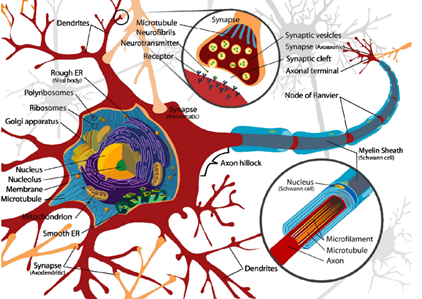
\includegraphics[width=10cm]{images/neuron1.png}
    \caption{Neuron}
    \label{fig:neurone_1}
\end{figure}
The \textit{central} part of the neuron is the part, which is managing the entire cell, this core the
\textbf{nucleus} is listening what is happening around the neuron,
when I have a \textbf{solicitation} from the external (other neurons or special cells related to the five senses).
\newline\newline
When there is sufficient stimulation coming from this cells the nucleus is solicited and at a given
point the nucleus realizes that the solicitation is so high that he has to
take an \textbf{action}, the action is to send a \textit{signal} around the \textit{axon} (the long extension covered in blue),
this will lead to have a \textbf{polarization} of an \textit{electric signal} which is flowing along this connection
and this will reach other neurons that are connected to the end of the axon to the synapses.
\begin{figure}[H]
    \centering
    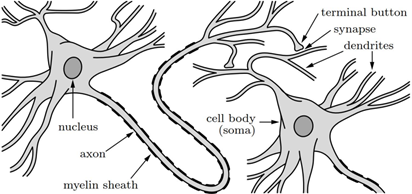
\includegraphics[width=10cm]{images/neuron2.png}
    \caption{Connection between two neurons}
    \label{fig:neurone_2}
\end{figure}
\noindent The \textbf{axon} is covered by an appropriate \textbf{protein} (covered in blue) which protect the axon itself,
and make sure that the polarization that occur on the nucleus is transmitted along the axon so that this signal is able
to reach the synapse.
\newline\newline
Basically, what we see is that the \textbf{neuron is exciting the nucleus}, which is generating the excitation along the axon,
then it will reach the terminal synapses.
\newline\newline
Each synapse is connected to the synapses of \textbf{another} neuron, so that the signals which are generated by
the nucleus and sent to the axon and then to the synapsis terminal at the terminal the synapses
are releasing some chemicals called \textbf{neurotransmitters}.
\newline\newline
These \textit{substances} are exciting the synapses of the connected neuron, but stimulating the synapses this excitation is
propagated from the \textbf{dendrites} to the nucleus of the other neuron, when the other cell is \textit{sufficiently excited} by
the amount of stimulation generated by the neurotransmitter the nucleus will generate again a new stimulation
which is going along the axon and reach another neuron (and so on...).
\newline\newline
Due to the fact that each neuron can stimulate each other neurons connected to them,
this will create the \textbf{parallel processing} in our brain, so that each component will take care
of analyzing each part of the information and this is a consequence to derive a part of the total computation.

\subsection{Computer vs Human brain}
When we look to the differences between a computer and the human brain what we notice,
is that in the computer we got processors composed by many \textbf{transistors}, the human brain counterpart
the got $10^{11}$ \textbf{neurons}, the number of the latter overcomes the number of the cores in a processor.
\newline\newline
The neurons aren’t able to process the same \textbf{complex operation} of a core, but they are still so many that they
can overcome the limit of the complexity of the individual operation with the fact that they are working significantly in
parallel.
\begin{figure}[H]
    \centering
    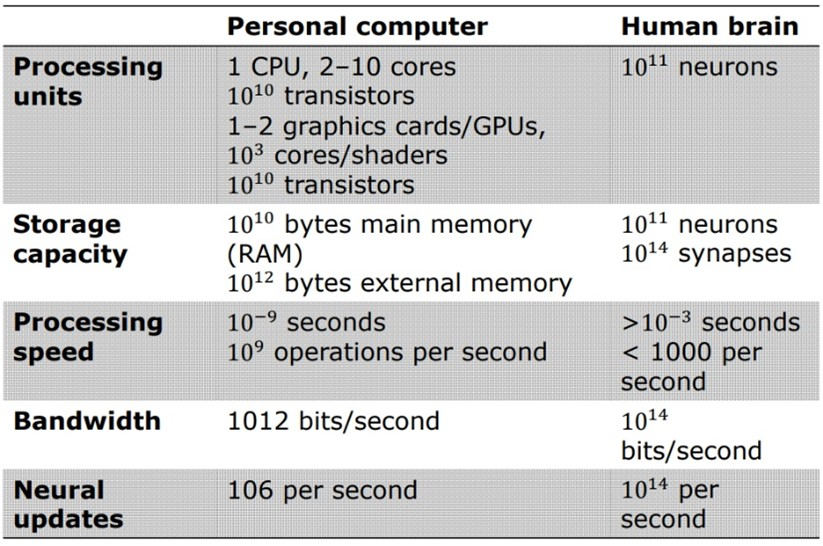
\includegraphics[scale=1.0]{images/tab_pc_vs_brain.jpg}
    \caption{PC vs Human brain}
    \label{fig:tab_pc_vs_brain}
\end{figure}
\noindent The \textbf{storage} of the neurons has an immense storage potential than any other memory capacity. The \textbf{processing speed}
seems \textit{much higher} on the computer, but the parallel operation that you can do in parallel in the human brain in
the end \textit{overcome} the processing speed of the hardware of a computer.
\newline\newline
Basically, what we can observe is that the biological neural networks are able to outperform significantly the processor that
we have nowadays, there are some researches carried out which are trying to create processors which are replicating in
hardware the operation of the biological neural networks but still the capabilities of this systems are \textit{far} from the
capability of human brain.
\newline\newline
It may \textit{seem} in some system that they are working faster then humans, it may seem that they are running better, but actually
what you have is that you have the ability in the computer to run the algorithms and the explore the
possible (deterministic) moves in a fast way but needs some background knowledge
in order to that in a very short time.
\newline\newline
Advantages of biological neural network:
\begin{itemize}
    \item High processing speed due to massive parallelism.

    \item Even if we have a significant amount of the biological neural network damaged, the system is
          considered \textbf{fault tolerance}, it remains functional even if larger parts of the network get \textit{damaged} (maybe some functions will be disabled).
          The other cells are able to overcome the death cells, this thanks to the elasticity of the neurons which are able
          to overcome possible damages in the structures.

    \item If more neurons are failing, the brain will \textit{degrade the performances} in a \textit{graceful way},
          it will not just stop working, will work a bit less not with the same performance and the same functionality
          but with reduced function. Only when a \textit{really massive} number of neurons is dying at that point a
          function is not working anymore.

    \item They are well suited for inductive learning (\textit{learning from examples, generalization from instances}).
\end{itemize}
What we are trying to do with artificial neural networks is to capture the parallel operation of the brain. The ability to
extract the knowledge from the data, we want to replicate these capabilities.
\newline\newline
There are some problems due to the \textbf{ANN} (artificial neural networks), if we kill part of the architecture which
is replicating the \textbf{BNN} (biological neural networks), the ANN is \textbf{not automated to survives}, we have to
assure some physical redundance, this is a problem of the architecture we are using to execute the computation of the ANN.
\newline\newline
What we want to do in our model is to construct a \textit{set of abstract models of the neurons} that we call
\textbf{artificial neurons}, and we like to connect them together to replicate the structure that we have in the
natural brain this is why we have the ANN, a connection of neurons that is trying to mimic the behavior of the brain.
\newline\newline
The complexity of the brain is so high that is actually difficult to replicate everything in ANN,
what we are doing is to replicate a specific function of the brain which is able to solve a specific application
problem that we have.
\pagebreak
\subsection{Threshold Logic Units}
This is the first \textit{abstract model} for an artificial neuron of the brain.
A \textbf{threshold logic unit} (TLU) is a \textit{processing unit} (neuron) with several inputs.
It can solve a very simple set of problems.
\newline\newline
We have a \textbf{core} (the neuron) with several \textit{inputs} that are reaching the neuron, and we have the
\textit{output} which is delivered to the subsequential neurons which are connected with it.
A TLU is a processing unit in which the output is governed by a threshold $\theta$, if it has a \textit{sufficient excitation}
from the inputs, then the TLU became \textbf{active} (value $1$) and generates the output $y$.
\begin{figure}[H]
    \centering
    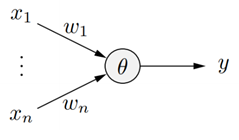
\includegraphics[width=6cm]{images/tlu.png}
    \caption{Threshold logic unit}
    \label{fig:tlu}
\end{figure}
We have $n$ inputs identified by $x_1,...,x_n$ the unit is generating only one output $y$ each input is \textbf{not}
delivered directly to the core of the TLU, but each input is \textbf{weighted}, some are more relevant,
and others are less relevant (exactly how we are doing when we consider the data from the external world).
\begin{figure}[H]
    \centering
    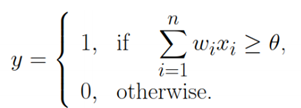
\includegraphics[width=6cm]{images/tlu_working_system.png}
    \caption{TLU conditions}
    \label{fig:tlu_conditions}
\end{figure}
This means that our problem is depending on the most important information, this is what happens in the real world.
\newline\newline
In the ANN we are replicating the relevance of the individual input, we can control how much each input is actually
important to influence the generation of the output, to do this we use a weight $w$ for each of the input so
that the TLU will not see exactly the input but will see a weighted input, this will allow the modulation of
each input by giving to each of them the appropriate importance during the generation of the final output.
\newline\newline
When the TLU is solicited enough it will generate an output $y$ that will be delivered to the \textit{terminal synapse}
to another neuron.
\begin{itemize}
    \item If the \textbf{excitation is enough}, mathematically means that the weighted summation is greater
          than a thresh $\theta$, we generate $1$ (the neuron is active).
    \item If the \textbf{excitation is not enough} for overcoming the threshold $\theta$, we generate $0$.
\end{itemize}
This model that tries to represent what is happening in the BNN from two scientists, also called the \textbf{McCulloch-Pitts neuron}.
\subsubsection{Conjunction example}
The result is equal to $1$ only when the two outputs are equal to $1$.
There is not a standard way to select the threshold $\theta$, we have to choose that in base of the
function that we want to implement. In this case I have to select a $\theta$ which is greater than the biggest weight.
$$x_1\land x_2$$
\begin{figure}[H]
    \centering
    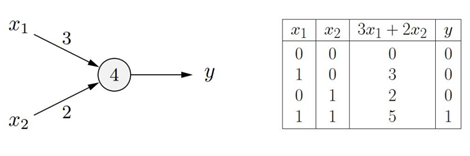
\includegraphics[width=10cm]{images/conj_TLU.png}
    \caption{Conjunction TLU}
    \label{fig:tlu_conjunction}
\end{figure}

\subsubsection{Implication example}
I can choose the value of the threshold in order to have the proper function, in this case applies on the same ways.
\textit{How can I choose the interconnection weights?}
\newline\newline
The problem is that there are no general rules, I choose the weights according to the intrinsic relevance of each
input variable.
\newline\newline
\textit{How can I do that when we have a high number of inputs?} we will see that there is a procedure for doing that.
$$x_2\rightarrow x_1$$
\begin{figure}[H]
    \centering
    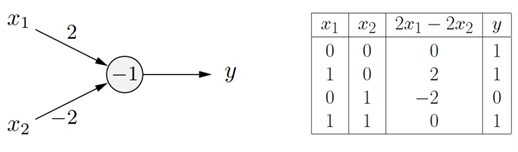
\includegraphics[width=10cm]{images/impl_TLU.png}
    \caption{Implication TLU}
    \label{fig:tlu_implication}
\end{figure}

\subsubsection{Multiple inputs example}
In this case we can see that we have three possible inputs, we can discriminate the
inputs in excitatory input and inhibitory input. The first tries to contributes
to the final computation of the neuron in such a way that the results
will be greater than the threshold, the other neuron does the opposite.
\begin{figure}[H]
    \centering
    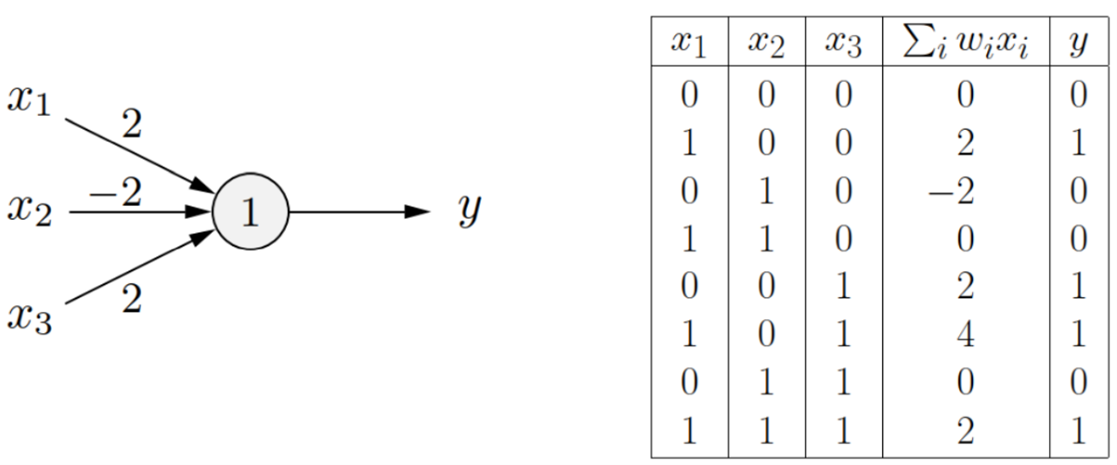
\includegraphics[width=10cm]{images/complex_TLU.png}
    \caption{Three-input TLU}
    \label{fig:tlu_3_input}
\end{figure}

\subsection{Geometric interpretation}
The geometric interpretation is significantly helpful to derive a \textit{method} to
configure the threshold and the weights starting from the data. We will consider a
single and simple TLU, we will try to understand how we can interpret the
behavior of the TLU in a geometrical way.
\newline\newline
You know that is possible to represent a straight line on a plane in any of
the following forms:
\begin{figure}[H]
    \centering
    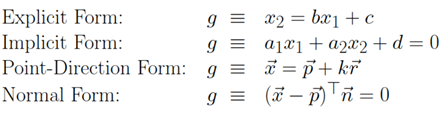
\includegraphics[width=10cm]{images/geom_interp.png}
    \caption{Different form for representing a straight line}
    \label{fig:line_repr}
\end{figure}
In the case of the \textbf{implicit form}, where you have a weighted combination of the two variables plus a
possible threshold, a vector representation in point-direction form and normal form.
Any of this is fine to represent a straight line in the plane, we are considering just
two variables $x_1$ and $x_2$, and use one of the many representations.
\begin{figure}[H]
    \centering
    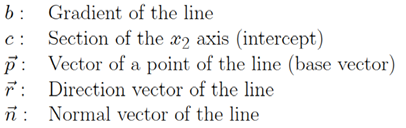
\includegraphics[width=9cm]{images/geom_interp_impl.png}
    \caption{Implicit form representation legend}
    \label{fig:line_impl_form_legend}
\end{figure}
\begin{figure}[H]
    \centering
    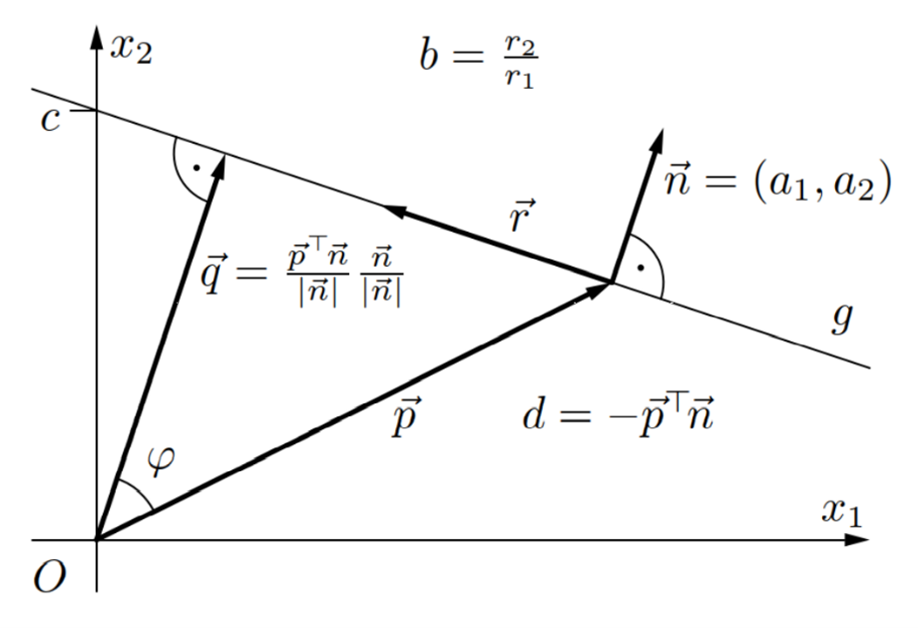
\includegraphics[scale=0.6]{images/geom1.png}
    \label{fig:geom_1}
\end{figure}
In the case of the \textit{explicit/implicit form} the $\vec{b}$ is the \textbf{inclination}
(or \textit{gradient}) of the straight line in respect of the horizontal axis,
and $c$ is the intercept of the vertical axis.
\newline\newline
If we look to the normal $\vec{n}$ we want to pick the vector which is \textit{orthogonal}
to the straight line. The straight line is represented by all the points which starts from the
origin and has a quantity in the direction of the normal. The vector $\vec{p}$ identifies a
point in the example, we consider that point belonging to our straight line,
the distance of the straight line respect to the origin $O$ is given by $|\vec{q}|$ which is
the projection of $\vec{p}$ on straight line $g$.
\begin{figure}[H]
    \centering
    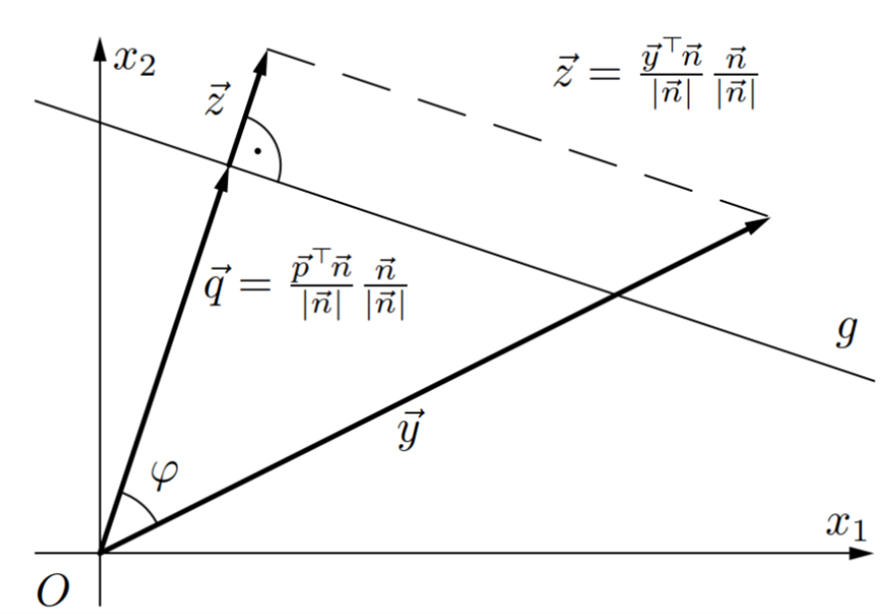
\includegraphics[scale=1]{images/geom2.png}
    \label{fig:geom_2}
\end{figure}
Considering this other graphical representation it is possible to know on which side
a points lands. If we take the vector representing $\vec{y}$ a point,
and I compute the projection in the direction of the normal, the projection
of this is the vector $\vec{z}$.
\newline\newline
To understand on which side the points are, I just need to see if the vector $\vec{z}$ (which is the
projection of our point) is shorter or longer than the point I observe on the straight line, which
is pointed by $\vec{q}$. This means that all points (expressed by a vector) which have a \textbf{module}
higher then the projected point onto the straight line ($\vec{q}$), are part of the plane above the
straight line (they will \textit{satisfies} the solution), viceversa, they will be below the plane if the
module will be shorter then $\vec{q}$ (they won't satisfy the condition).
\newline\newline
Basically the straight line which defines the behavior of my TLU, splits the plane in two parts (since I'm
considering only $x_1$ and $x_2$). All the points which distance is greater then
\begin{figure}[H]
    \centering
    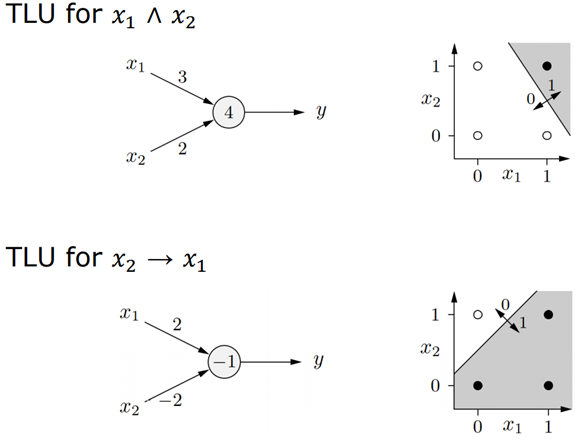
\includegraphics[scale=0.8]{images/tlu_examples_interp.png}
    \caption{Solution of the \textit{conjunction} and \textit{bi-implication}}
    \label{fig:example_interp}
\end{figure}
Now Let’s go back to the two examples that we have seen before,
starting with the conjunction, in this means that I have three points in which the output
has to be $0$, and one point where the result is $1$. This means that if I represent the straight
line with $x_1=3$, $x_2=3$ and the intercept equal to $4$ I will draw a line which is actually
separating in a clear way the element in which the output is equal to $1$ from the values
where the output is equal to $0$.
\newline\newline
For the case of three variables, this is more complex, we need to generalize this idea moving from
a plane to a three-dimensional space. Think about the three axis and look at the combination of the
dots, you need to set a plane, so you have to separate one set of inputs for which the output has
to be equal to $1$ from the set of inputs combinations where the output is equal to $0$.
\begin{figure}[H]
    \centering
    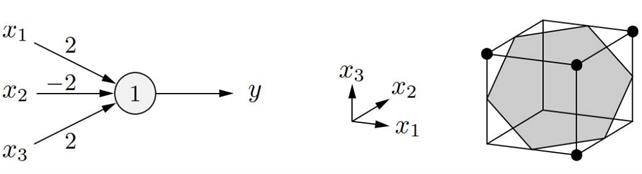
\includegraphics[scale=0.6]{images/three_input_sol_example.png}
    \caption{Solution of the complex TLU}
    \label{fig:example_three_sol}
\end{figure}
Basically, if you represent the plane using these information’s you will have this
kind of plane (that looks like a hexagon) dividing the solution from the $0$ values.
\newline\newline
\textit{So how we choose the threshold and interconnection weights?} I have to look at geometrical
distribution of the points for the combination of the input which the output must be equal to $1$
and the one where the output must be equal to $0$, I have to take a straight line or plane and I
need to position the divisor in a way that I clearly separate the two groups. If I can do that,
that set of values (inputs and threshold) are the one that I need to use in my ANN.
\begin{figure}[H]
    \centering
    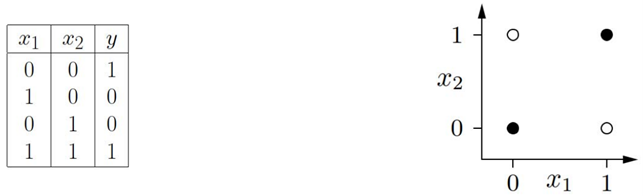
\includegraphics[scale=0.6]{images/bi_implic_no_sol.png}
    \caption{The bi-implication problem}
    \label{fig:bi-impl-problem}
\end{figure}
Let’s analyze another example, the bi-implication problem, this problem results in this kind of
distribution in the plane, as you can see it is not possible to separate these points with a
straight line. As a consequence, we don’t have any TLU for solving this problem, even if this is
a simple problem. We have to introduce some notions for understanding the reasons behind
this problem.
\subsubsection{Linear separability}
Two set of points in the \textbf{Euclidean Space}, consider $x_1, x_2,...,x_n$ as the variable for
the TLU, since we have $n$ possible inputs you are analyzing a problem represented in $n$
dimensional Euclidean space.
\newline\newline
If you have in this Euclidean space two set of points they are \textbf{linearly separable},
if and only if there exists at least one point, line, plane or hyperplane, such that all
points of the first set lie on one side and all points of the other set lie on the
other side of this point, line, plane or hyperplane.
\newline\newline
The point sets can be separated by a linear decision function.
\newline\newline
If you are in a mono dimensional space you have one input only,
your Euclidean Space is a line, you have one point on this straight line which is separating
your space the line in two parts, the output is one, for the other point the output is $0$.
If you have a plane, we have two input variables, we have to find a plane that separates
the two sets of points.

\subsubsection{Convex hull}
In a Euclidean space a \textbf{convex set} is a set in which, for each pair of points,
the segment that connects them is entirely contained in the set.
\newline\newline
A set of points $X$ is a \textbf{convex hull} in a Euclidean Space is the smallest convex set of
points that contains $X$. Alternatively, the convex hull of a set of points $X$ is the intersection
of all convex sets that contain $X$.

\subsection{Solution of the bi-implication problem}
Two sets of points in Euclidean Space are linearly separable if and only if their convex hulls
are disjoint. In the bi-implication problem, the convex hulls are the diagonal line segments.
\newline\newline
They share their intersection point and this means that they are not disjoint, therefore
the double implication is not linearly separable.
\begin{figure}[H]
    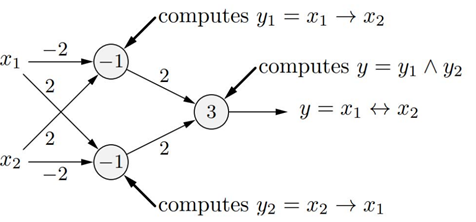
\includegraphics[scale=0.6]{images/sol_bi_implic_problem.png}
    \centering
    \caption{TLUs to the bi-implication problem}
\end{figure}
\noindent
What we can do is putting together more neurons to try to address more complex problem where
one neuron can’t solve. We are creating a network of TLUs, we are splitting the problem in two
sub problems.
\newline\newline
The problem of implication can be solved with a single TLU, we create a more complex structure
in which are able to solve the problem.
\newline\newline
Let’s see what happens geometrically, the two points $a$ and $c$, are going to be separated
from the first two  TLUs, I set one of the TLU so that all points which are below the straight
line represented by $g_2$ fives and output equal to $1$, and then I set a second straight line
represented by $g_1$ where all points are all over the straight line the values are equal to $1$,
and then I merge this information.
\begin{figure}[H]
    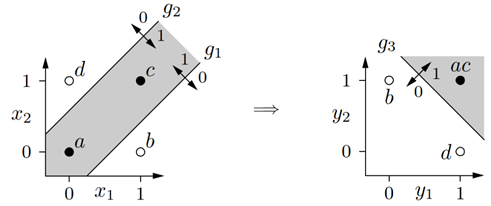
\includegraphics[scale=0.8]{images/sol_bi_implic_problem_graph.png}
    \centering
    \caption{Solution of the bi-implication problem}
\end{figure}
I combine these information from the previous group in the third neuron so that I transform
the representation of the information, I can merge the information of the points $a$ and $c$,
so that both the output of the two TLU is equal to $1$ is represented by one points (in this case
they are the same) and then I have the two other points $b$ and $d$ which are in both the parts
above and below the line, for them the solicitation is not enough to generate an output
equal to $1$, as a consequence I obtained a linear separability.
\newline\newline
I transformed the stripe in a semi plane with the third TLU, which identifies the linear
separability, I don’t have that propriety only with the first TLU but also with the second,
both TLUs allow me to partition the first space in three parts.

\subsection{Arbitrary boolean functions}
I can work with any arbitrary \textbf{Boolean function}; in this example I have a
Boolean function of three variables. I have these values of the value $y$ according to the formula.
\begin{figure}[H]
    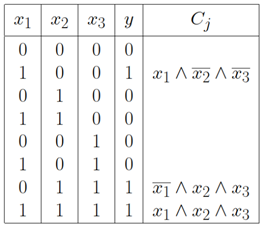
\includegraphics[scale=0.6]{images/arb_bool_funcs.png}
    \centering
    \caption{Table of values}
\end{figure}
What we can do is to build a network of TLUs that allow me to compute each of the component
for which the output has to be $1$ and then with a conjunction unit I put together all
the possible value with a or for merging the individual TLUs.
\begin{figure}[H]
    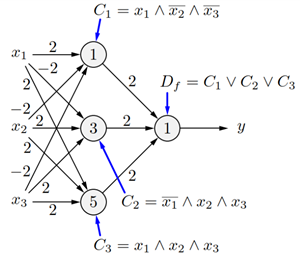
\includegraphics[scale=0.8]{images/arb_bool_funcs_graph.png}
    \centering
    \caption{Network of TLUs solving the boolean function}
\end{figure}

\pagebreak
\subsection{Training TLUs}
The geometric interpretation that we have seen before about the operation of TLUs gives us the
understanding of how we can place the various parameters for our networks in order to
construct TLUs with $2$ and $3$ inputs.
\newline\newline
But this makes sense when we are using $2$ or $3$ input, but this is something that is not
feasible when we are having more than three inputs, also this is not an automated method.
\newline\newline
We want an automatic method for visualizing the space and points in the space, especially when
we have more then $3$ inputs.
\newline\newline
What we want to do is to have an automatic way which adjusts the weights and the threshold
of the network so that I can reach the desired solution (if the two sets are linearly separable).
\newline\newline
The \textbf{automatic training} of TLUs consist in the fact that we can start from a random value
of the weights and threshold, and then when we want to configure a TLU we need to evaluate
the error that we are generating at the output (of the TLU) in respect to the input pattern
that we have presented.
\newline\newline
Basically, we have chosen randomly the threshold, the TLU generates an output, we evaluate
the error respect to the desired output, and then we try to adjust the weights and the
threshold to reduce the error.
\newline\newline
We repeat this operation for all inputs until the error is really reduced or vanished.
\begin{enumerate}
    \item Start with random values for weights and threshold.
    \item Determine the error from the output of the TLU.
    \item Consider the error as a function of the weights and the threshold $e=e(w_1,...,w_n,\theta)$.
    \item Adapt weights and threshold so that the error becomes smaller.
    \item Iterate adaptation until the error vanishes.
\end{enumerate}

\subsubsection{Negation example}
\begin{figure}[H]
    \centering
    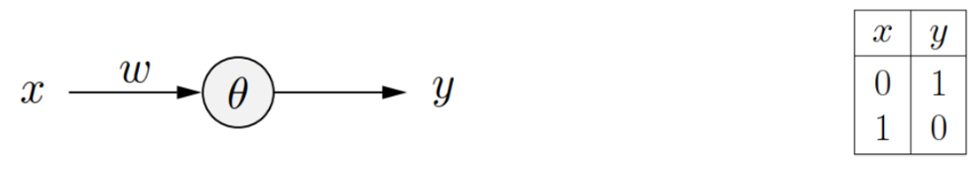
\includegraphics[scale=1]{images/neg_example.png}
    \caption{TLU that perform negation}
    \label{fig:neg_example}
\end{figure}
$$\neg x$$
In this case we have two really simple parameters, the weights and the threshold.
Let’s represent the error for all possible weights and all possible threshold at least
for a subset that we are interested in analyzing. Let’s consider the $x=0$, in this case
the desired output is $1$, if we take $w=2$ and we multiply it by $0$ the weighted input
will be $0$.
\begin{figure}[H]
    \centering
    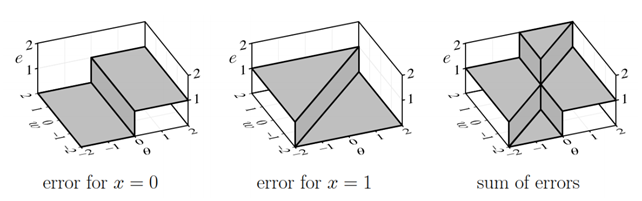
\includegraphics[scale=0.7]{images/errors_exampl.png}
    \caption{Diagrams of the errors expressed in terms of $\theta$ and $w$}
    \label{fig:neg_tlu_errors}
\end{figure}
Let's consider the first diagram on the left, with the various values of $\theta$ and $w$, and
with an input value of $x=0$.
Let's see the error that we have with the various possible combinations, we see that
for any values of the weight where the threshold is \textit{less} than zero, the \textbf{error}
is zero. Viceversa, for any value of the weight for a $\theta$ greater or equal to zero, the
error is one (a \textit{plateau}).
\newline\newline
Now let's consider $x=1$, we are on the central diagram, in the left triangular part
of the domain there will be the error of $1$ defined $\forall w$.
\newline\newline
Let's try to sum the errors and see what we obtains: we get an intersection for the error
equal to one, and also an intersection for the error equal to \textit{two} (which is strange,
since the error in this kind of example is always $1$ since the $y$ output is binary, but there
we are talking about a sum).
\newline\newline
The only part where the error is equal to zero is a small triangle on the bottom. The problem
with this definition of the error is that is not suited for define an algorithm which allow
me to find the zero error.
\begin{figure}[H]
    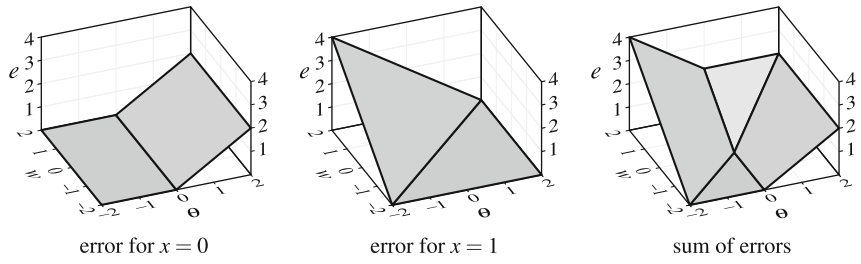
\includegraphics[scale=0.5]{images/desc_2_of_error.png}
    \centering
    \caption{Output error modified as function of weight and threshold}
\end{figure}
What I can do is modify the description of the error and consider that for each value
of the input I will not have just the error which is $1,0$ or $2$, but I will consider
a covering and continuos \textbf{surface area} (such that is possible to increase progressively
the error).
\begin{figure}[H]
    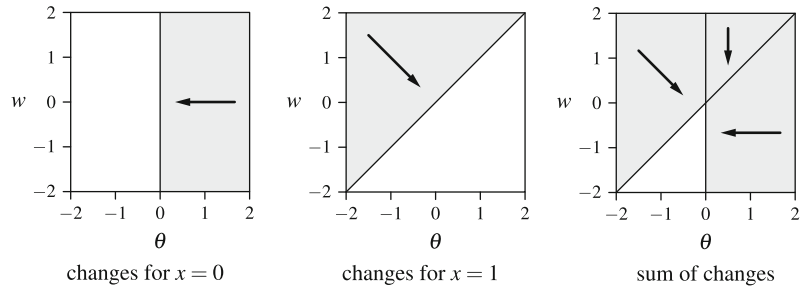
\includegraphics[scale=0.6]{images/desc_2_of_error_topview.png}
    \centering
    \caption{Top view output error modified as function of weight and threshold}
\end{figure}
So I can start from a random point and iteratively adapt parameters according to the direction
corresponding to the current point, I will stop if the error vanishes.
\newline\newline
There are two ways of training a neural network:
\begin{itemize}
    \item \textbf{online learning}, we receive the learning pattern at time from the
          external environment, we compute the parameter corrections for this learning pattern (like
          we saw in the negation example) and in the end we apply the parameter corrections. In
          case of the \textit{negation}, first we adapt the weight and the threshold according to the left diagram,
          then we adapt them according to the middle diagram, then we adapt them again
          according to the left diagram and so forth until the error vanishes.

    \item \textbf{batch learning}, consists in not applying the changes immediately after every
          training example, but aggregating them over all training examples. Only at the end of
          a (learning/training) epoch, that is, after all training examples have been traversed,
          the aggregated changes are applied. Then the training examples are traversed again
          and at the end the weight and the threshold are adapted and so forth until the error
          vanishes.
\end{itemize}

\subsubsection{Delta rule (Widrow-Hoff)}
Given:
\begin{itemize}
    \item $\vec{x}=(x_1,...,x_n)^T$ be an input vector of TLUs.
    \item $o$ is the desired output for this input vector.
    \item $y$ the actual output of the TLU.
    \item $\eta$ as learning rate.
\end{itemize}
If $y\neq o$, then, in order to reduce the error, the threshold $\theta$ and the weight
vector $\vec{w}=(w_1,...,w_n)$ are adapted as follow:
$$\theta^{(new)}=\theta^{(old)}+\Delta\theta\text{, with }\Delta\theta=-\eta (o-y)$$
$$w_i^{(new)}=w_i^{(old)}+\Delta w_i\text{, with }\Delta w_i = \eta (o-y)x_i$$
$$\forall I \in \{1,...,n\}$$
The first equation is correction (delta) of the threshold and the second is the correction of the
weight. The variation is given by an expression which is proportional to the difference
between the actual and expected output (which is the error).
\newline\newline
The correction for the weight is proportional not only to the error but also to the input.
Essentially, if I have an actual output smaller then the desired one, I take the input
that are bigger, and I try to push them to contribute more to the excitation
of \textbf{threshold logic function} so that the output will be higher and as
consequence the error will be lower.
\newline\newline
The $\eta$ controls the speed of updates, the bigger is the bigger will be the update.
\begin{figure}[H]
    \centering
    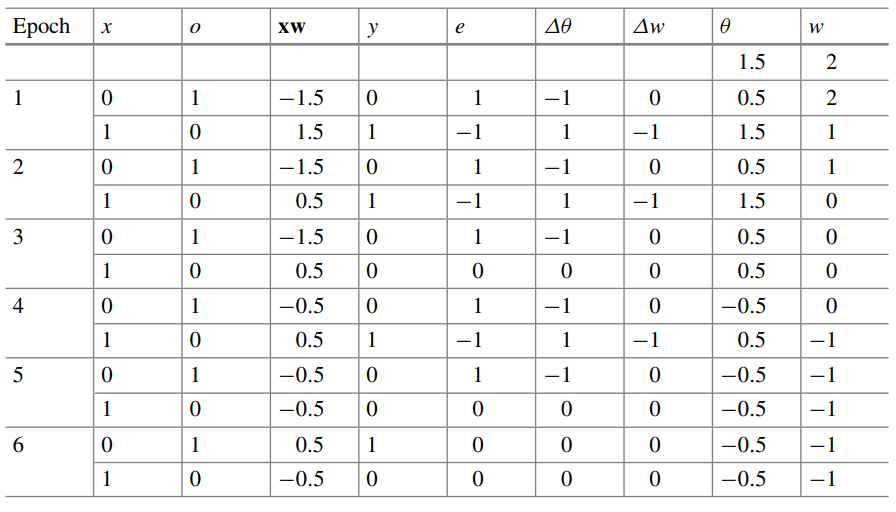
\includegraphics[scale=0.5]{images/online_training.png}
    \caption{Online training with $\theta = \frac{3}{2},w=2,\eta =1$}
\end{figure}
\begin{figure}[H]
    \centering
    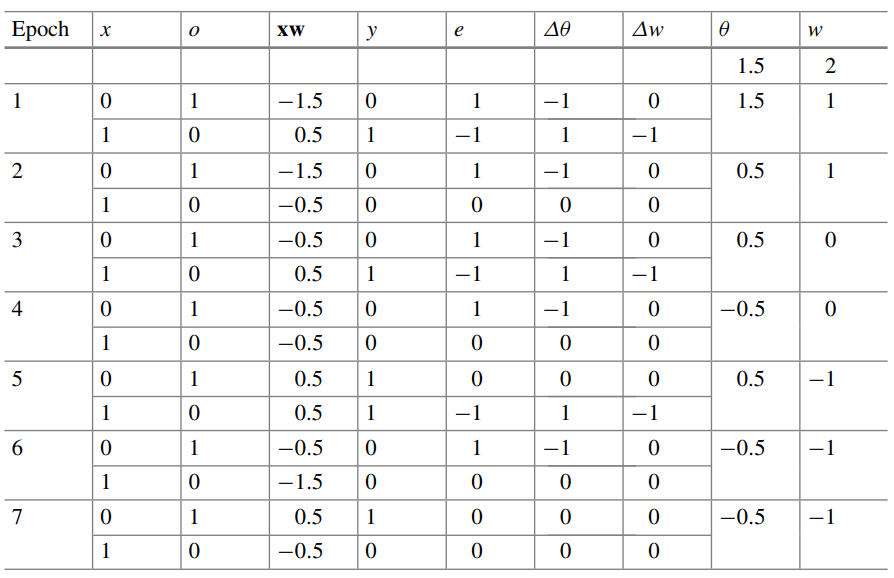
\includegraphics[scale=0.5]{images/batch_training.png}
    \caption{Batch training with $\theta = \frac{3}{2},w=2,\eta = 1$}
\end{figure}
Basically what happens in the online training, if I start in the first move I may go here,
and so on, I'll move one step at the time since the amount of change is control by the
learning rate.
\newline\newline
in this case I move in one direction, since I apply together the two errors correction,
so I'm moving in combination of the two changes of the secondo batch, then again I'm applying
the two changes and I move. I do less move respect to the other since  I combine the two
correction for the expression that I shown.
\newline\newline
I can try to do the same for the more complex case of the TLU, with two inputs. here I have
the conjunction with the truth table describing the implementation. What I'm doing basically
i have found the straight line that gives the satisfied and unsatisfied area for determining
the solution.

\subsubsection{Convergence theorem}
If we consider a set of training patterns: $L=\{(\vec{x_1},o_1),...,(\vec{x}_m,o_m)\}$,
each consisting of an input vector $\vec{x_i}\in\mathbb{R}$ and a desired
output $o_i\in\{0,1\}$.
\newline\newline
Furthermore, let's consider $L_0=\{(\vec{x},o)\in L|o=0\}$ and
$L_1=\{(\vec{x},o)\in L | o=1\}$. If I can show that $L_0$ and $L_1$ are
\textbf{linearly separable}, then is possible to prove that we have a
$\vec{w}\in\mathbb{R}^n$ and $\theta\in\mathbb{R}$ such that:
$$\forall (\vec{x},0)\in L_0 :\vec{w}^T\vec{x} <\theta$$
$$\text{and}$$
$$\forall (\vec{x},1)\in L_0:\vec{w}^T\vec{x}\geq\theta$$
This means that is possible to divide the two sets, and then the online or batch
training procedure is able to terminate. So if the two sets are linearly separable they
will give us a final value in a \textbf{finite time}. The final error will e zero.
\newline\newline
The problem is that if we are not able to perform the linear separation of $L_0$ and $L_1$,
the algorithm is \textbf{not able to terminate}. The algorithm will oscillate around and we
will not be able to find a solution with the zero error.
\begin{figure}[H]
    \centering
    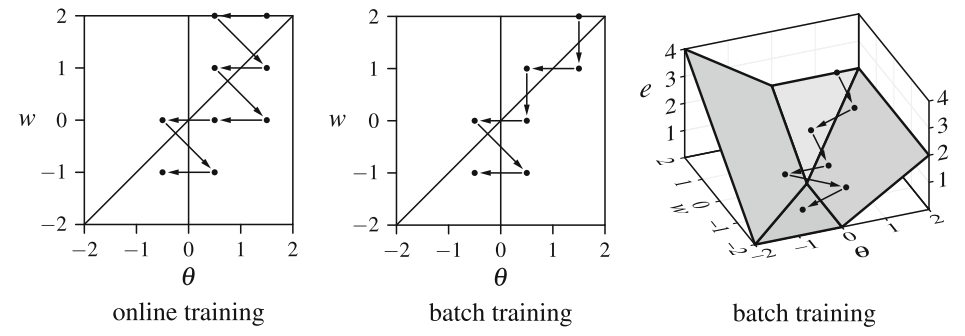
\includegraphics[scale=0.4]{images/batch_training_example_graph.png}
    \caption{Example of online and batch training (also with summed errors)}
\end{figure}
The correction of the parameters maybe slowed down due to the fact that we have $0$ and $1$
to the possible values for our outputs. This implies that if we have an output for our
threshold logic function equal to $1$, we can find an adjustment and apply it.
If we have an input which is $0$ whichever weight we have, we may not be able to compute
a correction that in the end will reduce the final error.
\newline\newline
So when we apply an input which is one we can change the weight for finding a better value
for the configuration, if we apply the change on an input which is zero the possible changes
actually vanishes since we are multiplying by zero, we are not observing a variation.
\newline\newline
To avoid to waste to much time on this issue, we can change the representation of the values,
for \textit{true} we are considering $1$ and for \textit{false} we are considering $-1$.
\newline\newline
What we can point out, is that a \textit{single} TLU, is able to point out any linearly
separable function. We have just to apply the delta rule which is easy and fast and
guarantee to find a solution, if one exists.
\newline\newline
The problem is given by a more complex structure, like a network of TLUs,
in this case we cannot apply directly the delta rule, because we have no clue
about which is the output. We need something more complex for managing that.

\subsection{Artificial neural network}
An ANN in general ha a very simple definition since it is a \textbf{directed}
graph $G=(U,C)$ composed by nodes and edges, in the graph we have processing
nodes that can elaborate the information incoming in, some arcs that
are bringing in the network some external information, and others that extract
the computation performed by our network (which is a structure that mimic our
brain).
\newline\newline
The connections are the axon-synaptic connections which connect the nucleus of the
neurons. In a general neural network this is the very abstract definition, in practice
in order to use this kind of structure we will need to have more regular more focused
organization of neurons connections.
\newline\newline
The set of vertices $U$ is partitioned into:
\begin{itemize}
    \item $U_{in}$ is the set of input neurons.
    \item $U_{out}$ is the set of output neurons, whi are the one delivering the
          result of the computation to the outside world.
    \item $U_{hidden}$ is the set of hidden neurons, they don't have any direct
          connection to the external world.
\end{itemize}

\subsection{General structure of the neuron}
\begin{figure}[H]
    \centering
    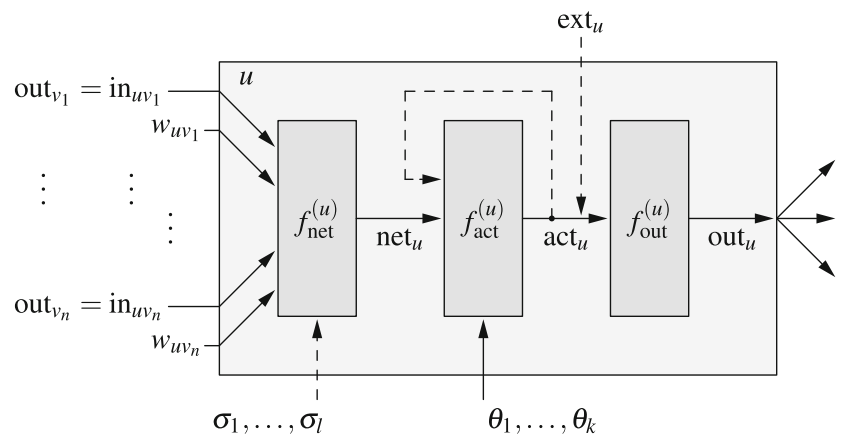
\includegraphics[scale=0.5]{images/general_structure_neuron.png}
    \caption{Internal representation of a neuron}
\end{figure}
We see that we have inputs that are coming in the network and usually this inputs are
manipulated in order to understand which is the global stimulus that the neuron
receive from the external world.
\newline\newline
If an incoming signal from a previous neuron has relevance, we want to multiply the
amount o signal incoming in by an appropriate constant in order to have a stronger weight
for a subsequent processing in this neuron.
\newline\newline
In this example we associate the weight $w_{uv_1}$, which is the weight for the neuron
$u$ respect to the incoming neuron $v_1$.
\newline\newline
These inputs are processed by three stages in which we perform specific operations, we want
to see how much the neuron is actually solicited. For these reason we have three
stage functions:
\begin{itemize}
    \item The $f_{net}^{(u)}$, takes the input with the \textit{relative relevance} of the
          various inputs to generate the \textbf{global solicitation} for our neuron. This is a general
          definition, a specific definition changes in base of the network we are considering.

    \item The $f_{act}^{(u)}$, the activation functions analyze the network input from the
          previous function and generate the \textbf{excitation status} of our neuron. This will tell
          us if the neuron is sufficiently excited.

    \item The $f_{out}^{(u)}$, which takes the excitation status of the neuron and elaborate
          the final status of the neuron to deliver to the subsequent neurons.
\end{itemize}
In general we have also an external variable $ext_u$ which tell us how much the excitation
should be increased from a stimulus coming directly from the \textit{external world}
(not from previous neuron, from the external world).
\newline\newline
These are the various inputs that any neuron can have, we may have both the input coming
from other neurons and the input coming from the external world, or we can have for a subset
of neurons only the stimulus coming from the external world and no other inputs.
\newline\newline
We have input neurons coming which are weighted properly, these values are used
with the \textit{network input function} which is generating the global excitation status
coming from the other neurons, this one is will generate the \textit{activation status} of the neuron (how much it is
stimulated by the external neurons).
\newline\newline
In the end we have the out function which evaluates the final status of the neuron, which
is delivered to the other connected neuron.

\subsection{Type of artificial neural network}
In the practice we won't use the general structure introduced before, we will have
different type of ANN:

\begin{itemize}
    \item \textbf{feed forward network} are ANN that doesn't contains any cycles, the
          acronym is FNN.
    \item \textbf{recurrent network} are ANN that contains cycles (backward connections),
          the acronym is RNN.
\end{itemize}

\noindent
The operation of a general ANN:
\begin{enumerate}
    \item \textbf{input phase}, where the external input are acquired by
          input neurons in the network.

    \item \textbf{work phase}, the external input are disconnect (by freezing
          the input neurons), we move the excitation generated by the input neurons
          to the connected neurons, we generate the stimuli for the connected neuron,
          we compute the output status of them and propagate the output to the
          neurons which are connected to this one.
\end{enumerate}
During the \textit{working phase} if the input of neurons are steady (input stimuli
are not changing), the computation of that neuron doesn't change (every stage
function generate the same values, FNN).
\newline\newline
This is not the case when we have a RNN, since if one of the outputs connected to
a neuron is connected to an input will repeat the computation and this maybe change
the output status (due to \textit{recomputation}). I always say \textit{"may"}
since the actual change will depend specifically by the function that I'm using.
\newline\newline
The \textbf{recomputation} of a neuron output occurs if any of its input changes,
we can't loop forever and not evolving. This means that the working phase continues
until the external outputs are steady, or a maximum number of
recomputation iterations is reached. The \textbf{temporal order} of computation
depends by the specific NN.
\newline\newline
\noindent\textbf{Feed-forward neural network}
\begin{enumerate}
    \item Computation proceeds from input neurons progressively toward output neurons by following
          the topological order of the neuron in the network.
    \item The external inputs are frozen.
    \item Input neuron compute their outputs which are maintained steady and forwarded
          to the connected neurons.
    \item Neurons connected to preceding neurons with steady outputs generate their
          respective outputs and propagated forward to the subsequent neurons, until the
          external outputs are generated.
\end{enumerate}
\noindent\textbf{Recurrent neural network}
\begin{figure}[H]
    \centering
    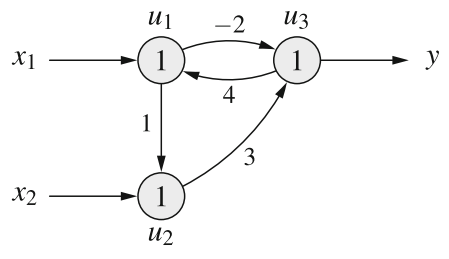
\includegraphics[scale=0.5]{images/RNN.png}
    \caption{A simple recurrent neural network}
\end{figure}
In the neurons there is the threshold which is considered for the operation,
and we have some interconnection weights which define the weights to be applied to the output
of a neuron when his output is delivered as input to a subsequent neuron.
\begin{figure}[H]
    \centering
    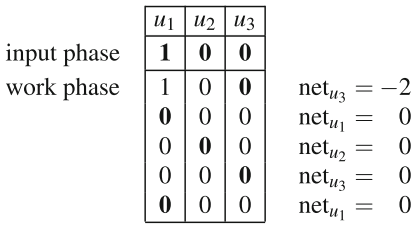
\includegraphics[scale=0.6]{images/RNN_simpl_ex1.png}
    \caption{Dataset for the previous RNN, for the $u_3,u_2,u_1$ order}
\end{figure}
In this case we choice to start from the input $1,0,0$ and with an updating order of
neurons that is $u_3,u_1,u_2,u_3,u_1,u_2,u_3,...$. Each bold number in working phase
entry of the table is an output of the \textit{ordered} neuron ($0$ if greater less than $\theta$
or viceversa $1$). In this case we can reach a steady state, and exit the RNN.
\begin{figure}[H]
    \centering
    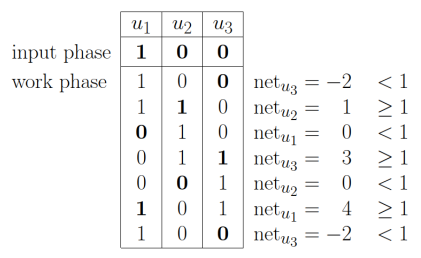
\includegraphics[scale=0.6]{images/RNN_simpl_ex2.png}
    \caption{Different dataset of the same RNN with $u_3,u_2,u_1$ order}
\end{figure}
Now let's consider a different ordering $u_3,u_2,u_1,u_3,u_2,u_1,u_3,...$, in this case
it is not possible to reach a steady state inside the RNN (\textbf{no stable state}, \textit{
    oscillation} of output).

\subsection{Configuration of a neural network}
The details of the configuration strictly depends from the
structure opf the network, in general we have two categories of
learning procedure (or training procedure):
\begin{itemize}
    \item \textbf{fixed learning task}.
    \item \textbf{free learning task}
\end{itemize}
\pagebreak
\noindent\textbf{Fixed learning task}
\newline
\noindent Considering a NN of $n$ input neurons $U_{in}=\{u_1,...,u_n\}$ and $m$ output neurons
$U_{out}=\{v_1,...,v_m\}$. A fixed learning task is a set of training patterns
$l=(\vec{i^{(l)}}, \vec{o^{(l)}})$, each consisting of:
\begin{itemize}
    \item an input vector $\vec{i^{(l)}} =(ext_{u_1}^{(l)},...,ext_{u_n}^{(l)})$
    \item an output vector $\vec{o^{(l)}} =(o_{v_1}^{(l)},...,o_{v_m}^{(l)})$.
\end{itemize}
\noindent At the end of the configuration the network is able to generate the desired output
that correspond to the output vector. Since the examples are composed by an input
vector and the expected output that we want to get, this is called \textbf{supervised
    learning}.
\newline\newline
A fixed learning task is solved when for all training patterns $l\in L_{fixed}$ the
neural network computes, from the external inputs contained in the input vector
$\vec{i^{(l)}}$ of a training pattern $l$, the outputs contained in the
corresponding output vector $\vec{o^{(l)}}$.
\newline\newline
\noindent\textbf{The error of a fixed learning task}
\newline
The error says how well a neural network solves a given fixed learning task. Essentially
it is the difference between desired and actual outputs.
$$e=\sum_{l\in L_{fixed}}e^{(l)}=\sum_{v\in U_{out}}e_v=\sum_{l\in L_{fixed}} \sum_{v\in U_{out}}e_v^{(l)}$$
$$e_v^{(l)}=\left(o_v^{(l)}-out_v^{(l)}\right)^2$$
In order to have a number which tell us the final quality what we need to do we have
to consider the module of the error, what we are doing is consider the difference between
the actual and the desired output. But in this simple difference could give us a final
number which is not reflecting the total accuracy of the NN due to the \text{sign}.
\newline\newline
A solution to this is to use a squared value, in this way we can avoid the negative
sign.
\newline\newline\noindent\textbf{Free learning task}\newline
A free learning task is the complementary approach of the fixed learning task, in
which the desired behavior is not defined a priori by the pair of vectors for
the input and the output.
$$n\text{ input neurons }U_{in}=\{u_1,...,u_n\}$$
$$\text{one input vector }\vec{i^{(l)}} = \left( ext_{u_1}^{(l)},...,ext_{u_1}^{(l)}\right)$$
We only have a set of input vectors which are presented to the network and the
learning algorithm will lead to an output vector which is similar to the given input.

\noindent\newline\textbf{Preprocessing}\newline
In order to be sure that the learning is working properly, we have to be sure
that one of the input is dominating the operation of the network, as consequence
we have to do some preprocessing on the data in order to give the same relevance
to all neurons.
\newline\newline
For each component of the input vector we need to compress the representation
in the same range, this is called \textbf{normalization} (according to the
average of the input value for each component, we need to be sure that
the variance $\sigma_k$ is normalized as well).
$$\mu_k =\frac{1}{|L|}\sum_{l\in L}ext_{u_k}^{(l)}$$
$$\sigma_k =\sqrt{\frac{1}{|L|-1}\sum_{i\in L}\left(ext_{u_k}^{(l)}-\mu_k\right)^2}$$
This is the standard normalization of the deviation $\sigma_k$, we have also another
possibility which is called \textbf{unbiased standard deviation} (often preferred
by statistician since is not polarized on the two direction).
\newline\newline
If we apply the normalization this is the external stimuli that we will have after
the normalization, basically all the stimuli are recomputed with respect to the
average value and they are normalized in dimension dividing them by the standard
deviation.
$$\sigma_{u_k}^{(l)(new)}=\frac{ext_{u_k}^{(l)(old)}-\mu_k}{\sigma_k}$$
There is a problem that we have to seriously consider when we are looking
to our examples, we need to have \textit{sufficiently descriptive examples},
which have to be well distributed over the domain that I'm considering (not
focussing only on a portion of the domain).
\newline\newline
So far we have been dealing with integer and real numbers, we want to use
symbols for represent a group of examples that are similar together in a concise way.
\newline\newline
For doing that we need to associate a group of identifiers to a group of examples. For
being able to represent this symbols we consider the \textbf{1-in-N encoding}, if
we need to represent $n$ symbols we have a string of $0$ and $1$ and only one bit the one
that corresponds to the symbol we want to represent will be $1$ (the others will be $0$).

\subsection{Multi-layer Perceptrons}
A \textbf{multi-layer perceptrons} it is essentially a feed-forward neural network
in which is present a strictly layered structure. They neurons are connected in groups,
each groups receives the input only from the previous layer or from the external input.
The output is delivered to the subsequent group, there are different kinds of layers:
\begin{figure}[H]
    \centering
    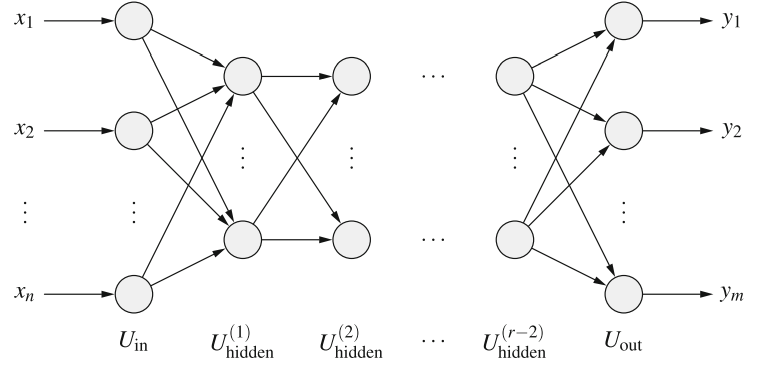
\includegraphics[scale=0.5]{images/multi-layer-percep.png}
    \caption{General structure of $r$-layered perceptron}
\end{figure}
\begin{itemize}
    \item \textbf{input layer}
    \item \textbf{hidden layer}
    \item \textbf{output layer}
\end{itemize}
Each layers is connected, in multi-layer perceptrons the neurons are strictly connected
between layers, jump are not allowed (like in the feed-forward network).
\newline\newline
The network input function of each \textit{hidden neuron} and of each \textit{output neuron}
is the \textbf{weighted sum} of its inputs:
$$f_{net}^{(u)}(\vec{w_u},\vec{in_u})=\vec{w_u}\vec{in_u}=\sum_{v\in pred(u)}w_{uv}out_v$$
The activation function of each hidden neuron is a so-called \textbf{sigmoid function},
that is, a monotonically non-decreasing function with:
$$f:\mathbb{R}\rightarrow [0,1]\text{ with }\lim_{x\rightarrow -\infty}f(x)=0\text{ and }\lim_{x\rightarrow\infty}f(x)=1$$
It has a shape that allows a minimum and a maximum value (shaped), such that the possible \textit{net status}
of the neurons is inside the continuos domain between $0$ and $1$ (this is called \textbf{squishification} of the net status).
If I have enough excitation in the network status the sigmoid function will give a positive excitation of the neuron,
viceversa, it will point out a lower value in the function.
\begin{figure}[H]
    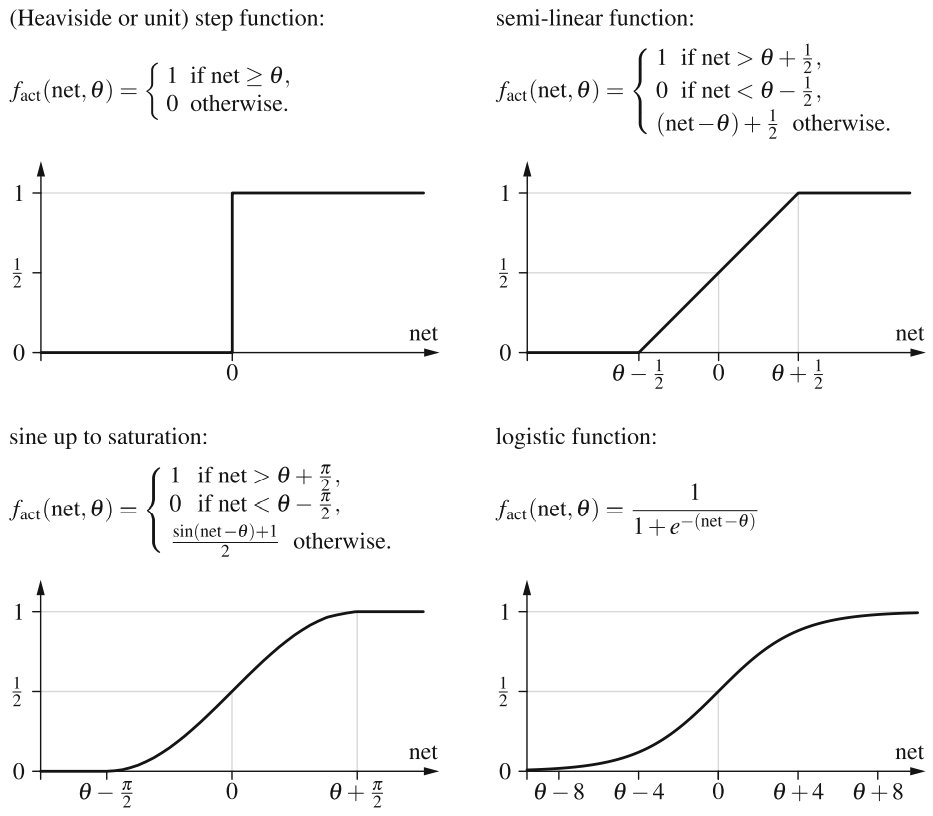
\includegraphics[scale=0.45]{images/sigmoid_functions.png}
    \centering
    \caption{Some \textbf{unipolar} sigmoid activation functions}
\end{figure}
In the contemporary NN the sigmoid function are rarely used, actually the \textbf{ReLU} (\textit{Rectified Linear Unit})
function is much more used since it is much easier to train (more similar to the behavior of the biological neurons).
\begin{figure}[H]
    \centering
    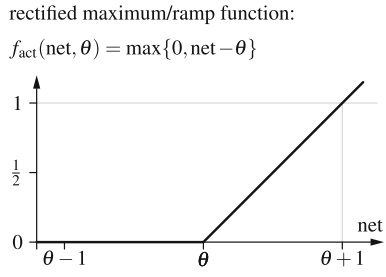
\includegraphics[scale=0.5]{images/relu.png}
    \caption{ReLU function}
\end{figure}
The output function of each output neuron can be a sigmoid or can be a \textbf{linear}
function (depends on what we want to achieve). There are many types of sigmoid function for representing
the general behavior, the most simple is the \textbf{step function}.
\newline\newline
I have a $0$ value until my network excitation reach the value $\theta$, then the output
of excitation jump to the strongest status (the value of minimum and maximum activation are
generally $0$ and $1$).
\newline\newline
If you prefer a smoother approach you can use the $sin$ approach were the derivative
is progressively approaching the maximum value.
\newline\newline
A \textbf{logistic} function is a function with the same shape but that doesn't reach a saturation
at the extremes of the range. In this way it is possible to consider the inverse
of the function, otherwise it is not possible.
\newline\newline
We may have some problems during the learning operation when using the \textit{step function},
since when we have $0$ we won't have any effect on the output of the neuron,
even if we change the activation the output will be $0$. As solution it is possible to
use \textbf{bipolar} (opposite to the unipolar, which extends only in one pole)
sigmoid functions, which changes the ranging to $[-1,+1]$, like the \textit{hyperbolic tangent}.
\begin{figure}[H]
    \centering
    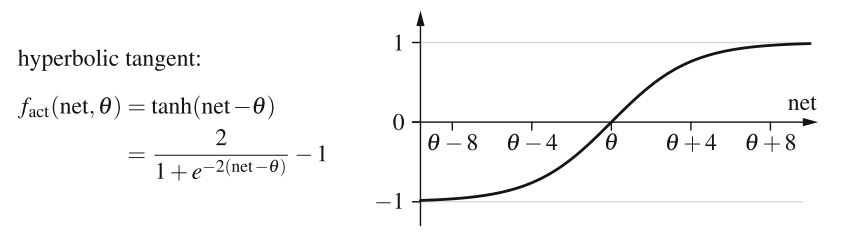
\includegraphics[scale=0.5]{images/hyperbolic_function.png}
    \caption{Bipolar sigmoid activation function (\textit{hyperbolic tangent})}
\end{figure}
I can describe the group of connections between two \textit{consecutive} layers of
a multi-layer perception by using a $n\times m$ matrix. Which is the collection of the
connection weights between the layers:
\begin{figure}[H]
    \centering
    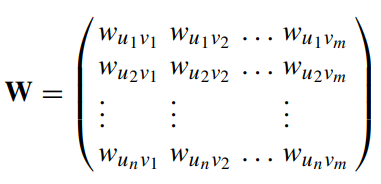
\includegraphics[scale=0.5]{images/weight_matrix.png}
    \caption{Matrix describing connection weights between two layers}
\end{figure}
As a consequence the computation can be described in a very simple way,
by using the vectors:
$$\vec{net_{U_2}}=\textbf{W}\vec{in_{U_2}}=\textbf{W}\vec{out_{U_1}}$$
You just take the vector of the input neurons of the second layer
(which are the output of the preceding layer) and multiply by the
weight in between the layers.
\newline\newline
Then you apply the sigmoid function $\sigma$ for squish the values between $[0,1]$,
you can also use a \textbf{bias} value for each independent values by using a vector $\vec{b}$.
The bias tells you \textit{how high} the threshold has to be in order for the neuron to fire.
$$\sigma\left(\textbf{W}\vec{in_{(U_2)}}+\vec{b}\right)$$
Let's consider an example with the \textbf{bi-implication}
three-layer perceptron:
\begin{figure}[H]
    \centering
    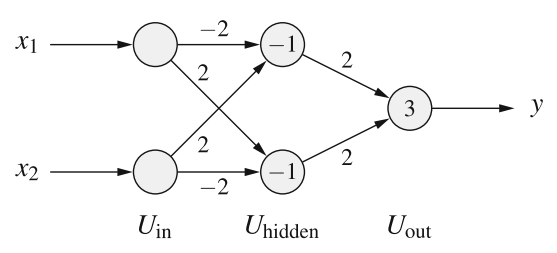
\includegraphics[scale=0.5]{images/three_layer_example.png}
    \caption{Three-layer perceptron for bi-implication}
\end{figure}
\begin{figure}[H]
    \centering
    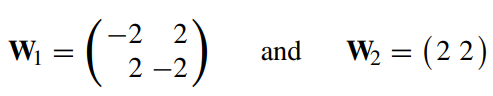
\includegraphics[scale=0.5]{images/weights_three_layer_example.png}
    \caption{Weight matrices for the input and hidden layers}
\end{figure}
The only difference respect the TLUs network of bi-implication is that
each neuron can be an input,hidden and output neuron. In this configuration
we are dividing everything in layer of neurons, so we have to \textbf{add} a
input layer for that (in respect to using TLU).
\newline\newline
So far we have seen boolean function, but what we want to look now is how we can extend
the dimensions of a feed-forward network in order to consider not only
the boolean function of the TLUs but we want to consider in a multi-layer
perceptron any type of real number (extend the capability of describing the world).
\newline\newline
We can see that the multi-layer perceptron,
with any input real-number can be used for function approximation.
\newline\newline\noindent\textbf{Function approximation}\newline
Consider the function in the diagram, it is very simple and continuos,
and let's consider the points $x_1,...,x_4$ where we want to compute
the value of the function and we want to find a method to approximate for any other value
$x$ a value in that function.
\newline\newline
What I can do is to consider the \textbf{midpoint Riemann integration}.
\begin{figure}
    \centering
    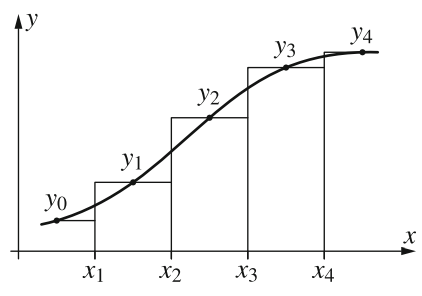
\includegraphics[scale=0.5]{images/midpoint_integra.png}
    \caption{Approximating a continuos function with step functions}
    \label{fig:midpoint_int}
\end{figure}
\begin{itemize}
    \item Approximate a given function by a step function.
    \item Construct a neural network that computes the step function.
    \item Error is measured as the area between the functions.
\end{itemize}
It is possible to prove that if you take any Riemann integrable function,
it can be approximated with arbitrary accuracy by a \textit{four-layer perceptron}.
\begin{figure}[H]
    \centering
    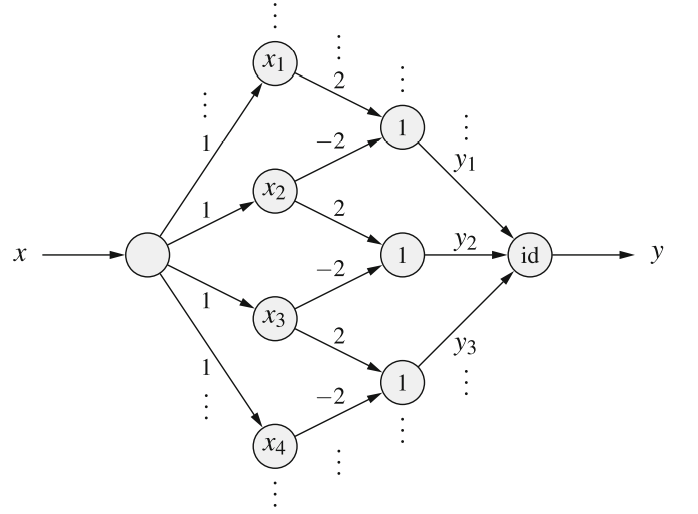
\includegraphics[scale=0.5]{images/integra_perceptron.png}
    \caption{NN that computes the step function for integration}
\end{figure}
The input $x$ is taken by an input neuron, then we have the first
layer composed by the subdivision of the domain in the points
$x_1, x_2, x_3,x_4$.
In the second hidden layer, we create one neuron for each step,
which receives input from the two neurons in the first hidden layer that
refer to the values $x_i$ and $x_{i+1}$ marking the border of the step.
Only one neuron in the second layer can be active, and it will represent
the step where the input values lies (this through the \textbf{combined
    excitation} of the neurons in the first hidden layer).
\newline\newline
The connection from the neurons of the second layer to the output
neuron are weighted with the function values of the stair steps that
are represented by the neurons.
\newline\newline
Since only one neuron can be active on the second hidden layer, the
output neuron receives as input the height of the stair step , in which
the input value lies, as result it computes the correct sampling
of the function saw in figure \ref{fig:midpoint_int}.
\newline\newline
The multi-layer perceptrons can be considered an \textbf{universal
    approximators} of the Riemann integration technique, with the maximum
desired error (i can choose the maximum error I want to get for my
function by choosing the number of neurons for get that accuracy).\newline\newline
\noindent\textbf{Delta approximation approach}\newline\noindent
We can actually simplify the error by considering a trick instead of using the
combined excitation.
\newline\newline
I can split the domain of the function for my network in parts like before,
then instead of defining the value of the function for each interval I just
use iteratively the $\Delta$ variation respect to the value considered.
\begin{figure}[H]
    \centering
    \caption{}
    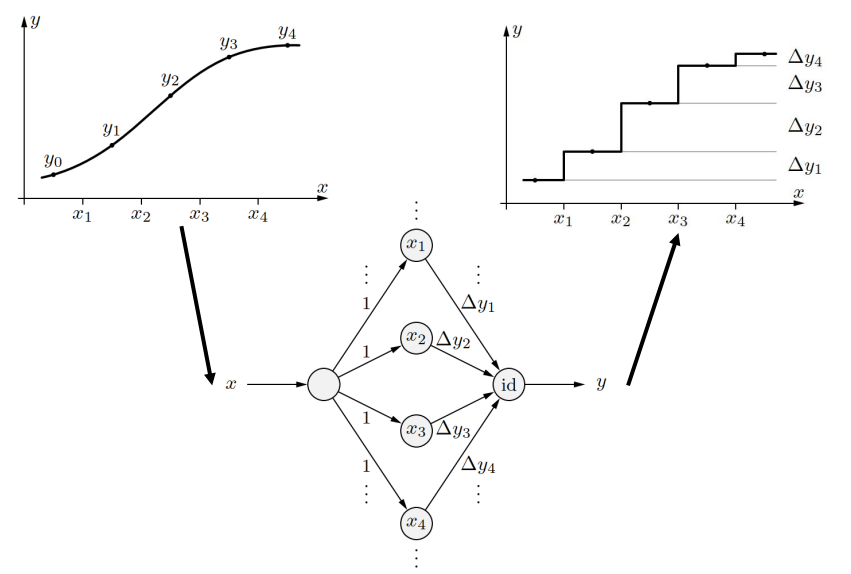
\includegraphics[scale=0.5]{images/multi-delta-integra.png}
    \label{fig:integra_delta}
\end{figure}
The structure of the network (figure \ref{fig:integra_delta}) will be simpler
because I will distribute the input of the hidden neurons,
that will tel me if the value $x$ is before $x_i$ or greater than $x_i$ (i don't care where).
\newline\newline
For example, if the value is between $x_1$ and $x_2$ the first neuron
will generate $\Delta y_1$ and this will be delivered in output.
\newline\newline
If I have a value between $x_2$ and $x_3$ I will still have $x_1$ that
will be excited enough and will generate the \textit{contribution}
for the output ($x_1$ and $x_2$ will be both excited, their
contribution will be summed up and then delivered to the output).
\newline\newline
This will make simpler the structure of the network.

\subsection{Regression}
Let's find a way for approximate a function without using the basic calculus approach. In
order to do this we have to understand the concept of \textbf{regression}.
We saw that for training an ANN we need to minimize the error function, which is computed by
considering the squared difference between desired output and actual output.
\newline\newline
The regression is a technique used in statistical analysis for extrapolating a straight
line that better approximate the existing relationship inside a dataset.
\newline\newline
Formally, considering the dataset $G=\{(w_0,y_0),...,(w_n,y_n)\}$ let's imagine it exists a functional relationship
between the input vector $w_i$ and the abscissa $y$, then the regression will help us to find
the parameters of that function. Different kind of functions will give us different kind of regressions.

\subsubsection{Linear regression}
If we expect that our quantities $x$ and $y$ exhibits a linear dependence, then we have
to identify the parameters $a$ and $b$ that extrapolate the straight line $y=g(x)=a+bx$.
In general, won't be possible to find a straight line that traverse all the points of the
dataset. What we will do is finding a straight line which deviates the lest possible,
so that minimize the error as follows:
$$F(a,b)=\sum_{i=1}^{n}(g(x_i)-y_i)^2=\sum_{i=1}^n(a+bx_i-y_i)^2$$
The necessary condition to find the minimum is given us by mathematical, if I take the
partial derivatives between the two parameters $a$ and $b$ (which are the variables
in the formula) setting this partial derivatives of th error to $0$ it will give to
me the condition that allow us to find the minimum (\textit{Fermat's theorem}).
$$\frac{dF}{da}=\sum_{i=1}^{n}2(a+bx_i-y_i)=0$$
$$\frac{dF}{db}=\sum_{i=1}^{n}2(a+bx_i-y_i)x_i=0$$
The \textit{linear algebra} tells me the solution is unique unless I'm so unlucky that
all the values $x$ coincides, in that case I have basically one equations but
two variable ($a$ and $b$) and as consequence infinite solutions.
\newline\newline
For example, if I need to find the regression of these points:
\begin{figure}[H]
    \centering
    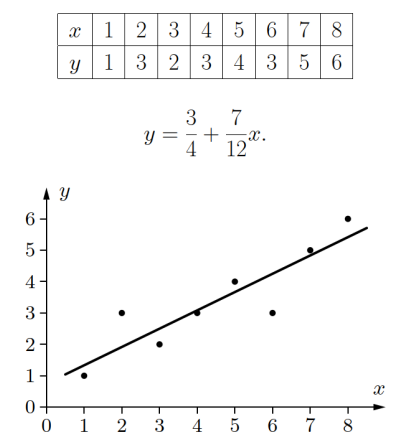
\includegraphics[scale=0.7]{images/regression_line.png}
    \caption{Regression line example}
    \label{fig:regression_line}
\end{figure}

\subsubsection{Polynomial regression}
The previous method is generalizable to polynomial of arbitrary order.
The model I have considered is not a good model, is too approximate, I can look if there
is instead a very simple straight line a polynomial.
Instead of considering a polynomial of grade one, I consider a polynomial of grade $m$.
$$y=p(x)=a_0+a_1x+...+a_m x^m$$
The minimization fo the error now can be generalized in this way:
$$F(a_1,...,a_n)=\sum (p(x_i)-y_i)^2=\sum(a_0+a_1x+...+a_n x^n-y_i)^2$$
Like in the linear regression, the necessary conditions for the function to be
minimized (finding the minimum), are that the partial derivatives respect to the
parameters $a_i$ vanishes:
$$\frac{dF}{da_0}=0,\frac{dF}{da_1}=0,...,\frac{dF}{da_m}=0$$
\begin{itemize}
    \item This system can be solved by using the standard methods from linear algebra.
    \item The solution is unique unless the points lie extactly on a polynomial of
          lower degree.
\end{itemize}

\subsubsection{Multilinear regression}
Until now I just tried to make the approximation more accurate going in the
direction of polynomial,\textit{what happens if I have a function in multiple variables?}
$$z=f(x,y)=a+bx+cy$$
If I want to do a multi-linear regression (since I'm applying linear regression to a function
of two variables), I have just to apply what I wast doing before.
\newline\newline
I have to consider the error in the approximated function $f$, and the actual value given
by the samples $z_i$ that I'm collecting (minimizing the sum of squared errors):
$$F(a,b,c)=\sum_{i=1}^{n}$$
What we need to do? again we need to find when the error is going to $0$, this happens when
the partial derivatives of the parameters are $0$.
$$\frac{dF}{da}=\sum_{i=1}^n 2(a+bx_i+cy_i-z_i)=0$$
$$\frac{dF}{da}=\sum_{i=1}^n 2(a+bx_i+cy_i-z_i)x_i=0$$
$$\frac{dF}{da}=\sum_{i=1}^n 2(a+bx_i+cy_i-z_i)y_i=0$$
As already said multiple times, the linear algebra will allow me to solve
this problem since I have three parameters $a,b,c$ and three equations.
\newline\newline
Except the unfortunate case where all points are on a straight line, because in this case
i have a plane that can be rotated in any direction and I have \textit{infinite solutions}.
\newline\newline
I can consider trying to approximate with a multi-linear regression a function that
is defined on $m$ different variables, this is the generalization of what we have
seen previously (difficult to draw):
$$y=f(x_1,...,x_m)=a_0+\sum_{k=1}^{m} a_k x_k$$
I have to minimize the sum of squared errors (vectors for parameters and matrices to define
the various values):
$$F(\vec{a})=(\textbf{X}\vec{a}-\vec{y})^T(\textbf{X}\vec{a}-\vec{y})$$
where:
\begin{figure}[H]
    \centering
    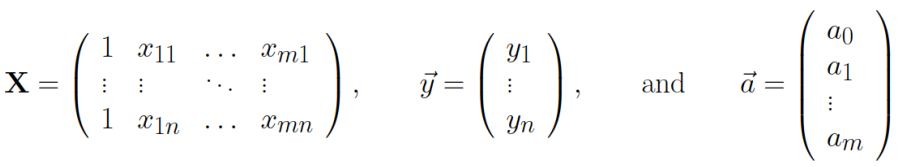
\includegraphics[scale=0.5]{images/parameters_multilinear_regre.png}
    \label{fig:infos_multilinear}
    \caption{Various $x$ values and vector parameters}
\end{figure}
I need to define the \textbf{gradient} which is the generalization of the previous definition
defined on vectors and not on the partial derivatives of functions as we seen before.
We need to look where the gradient is $0$ which will give us the \textit{hyperplane}
touching the surface in the minimum.
$$\vec{\nabla}_{\vec{a}} F(\vec{a})=\vec{\nabla}_{\vec{a}}(\textbf{X}\vec{a}-\vec{y})^T(\textbf{X}\vec{a}-\vec{y})=\vec{0}$$
This comes out as set of regular equations and linear algebra will allow us to solve it as
usual unless there is the singular case (if I have all points aligned to a single straight line
the plane which is minimizing my error is not defined).
\newline\newline
The system of normal equations:
$$\textbf{X}^T\textbf{X}\vec{a}=\textbf{X}^T\vec{y}$$
which has solution unless $\textbf{X}^T\textbf{X}$ is a singular:
$$\vec{a}=(\textbf{X}^T\textbf{X})^{-1}\textbf{X}^T\vec{y}$$

\subsubsection{Logistic regression}
In the situation in which the dataset is not approximated with sufficient accuracy
from a polynomial function, we could use different kind of functions, for example:
$$y=ax^b$$
We can transform this in a linear equation by applying the operation of logarithm:
$$\ln{y}=\ln{a}+b\cdot\ln{x}$$
In the case of ANN we are interested in particular at the \textbf{logistic function}:
$$y=\frac{Y}{1 + e^{a+bx}}$$
If we apply the logarithm of this equation we can derive a different expression of our
function $y$ so that the description of this function will be a \textbf{linear description}.
\newline\newline
Since lot of ANN uses as proper neuron activation function the logistic function,
if we would find a way for applying the regression method on that we could determine
the parameters of any network.
\newline\newline
If we would find a way for applying the method of regression om the neurons, we could
determine the parameters of any network at two layers of only one point. The value $a$
of the function represent the threshold of the output neuron, while the value of $b$
represent the weight of the input. We can linearize the logistic function by applying
the following transformations (called \textbf{logit transformation}):
$$y=\frac{Y}{1+e^{a+bx}}\longleftrightarrow\frac{1}{y} = \frac{1+e^{a+bx}}{Y}
    \longleftrightarrow\frac{Y-y}{y}=e^{a+bx}\longleftrightarrow\ln{\left(\frac{Y-y}{y}\right)}=a+bx$$
\begin{figure}[H]
    \centering
    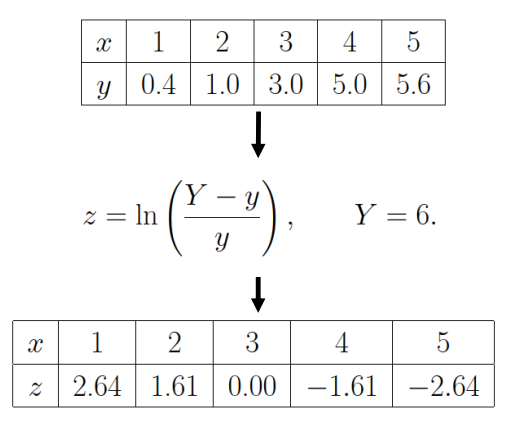
\includegraphics[scale=0.5]{images/logistic_regre_1.png}
    \label{fig:regr_1}
    \caption{Example of logistic regression}
\end{figure}
The results of the regression line in the example are:
$$z\approx -1.3775x+4.133, y\approx\frac{6}{1+e^{-1.3775x+4.133}}$$
\begin{figure}[H]
    \centering
    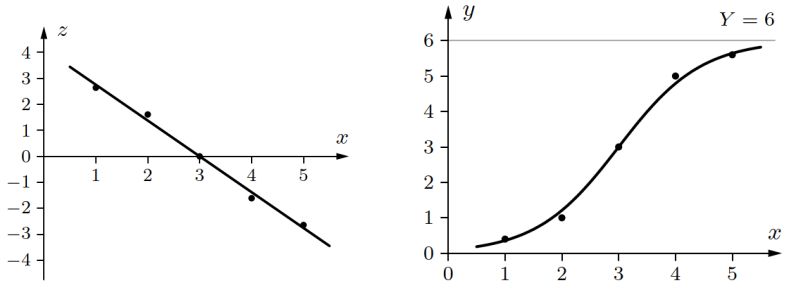
\includegraphics[scale=0.5]{images/regression_line_2.png}
    \label{fig_regr_2}
    \caption{Plot of logistic function}
\end{figure}
How can we understand the values of this non polynomial approximation by transforming it
applying the log transformation, so that we can perform the approximation on a
function that appear to be linear and then transform it back on the original function.
\newline\newline
We can consider a logistic function defined on two variables, and we have this bi-dimensional
shape defined on two arguments. we can apply the same principle that we see before, this
can be used to solve a problem of separating two groups of examples of different classes (or
group).
$$y=\frac{1}{1+exp(4-x_1-x_2)}=\frac{1}{1+exp\left(4-(1,1)^T(x_1,x_2)\right)}$$
\begin{figure}[H]
    \centering
    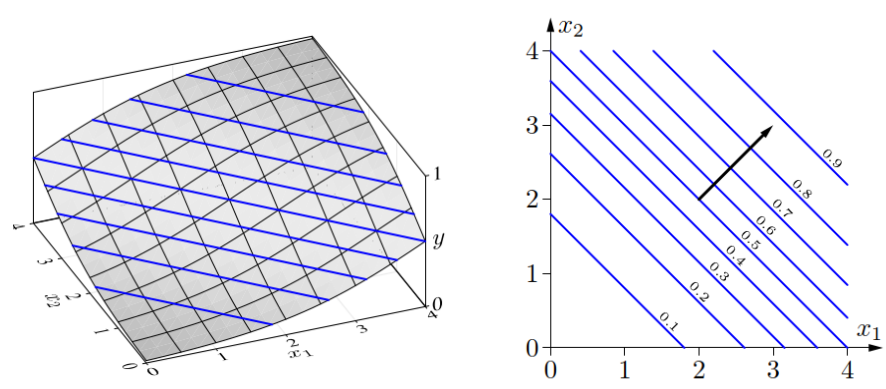
\includegraphics[scale=0.45]{images/logist_bidiminesional_reg.png}
    \caption{Plot of logistic function with two arguments}
\end{figure}

\subsubsection{Two-class problems}
Basically the two class problems can be solved by considering the two attributes,
which are the name of the class ($C$ is the class of attributes) and a vector random of $m$ dimension.
$$dom(C)={c_1,c_2}$$
We consider the \textbf{probability} of belonging to the first class $c_1$
and the probability to be in the second class $c_2$.
$$P(C=c_1|\vec{X}=\vec{x})=p(\vec{x})$$
$$P(C=c_2|\vec{X}=\vec{x})=1-p(\vec{x})$$
Given a dataset of points $X={\vec{x_1},...,\vec{x_n}}$, each of which belongs to one
of two classes $c_1$ and $c_2$.
\newline\newline
Basically I want to get a \textbf{simple description of the function} $p(\vec{x})$, if I have
this function I can apply the \textbf{logistic description}:
$$p(\vec{x})=\frac{1}{1+e^{a_0+\vec{a}\vec{x}}}=\frac{1}{1+exp(a_0+\sum_{i=1}^m a_i x_i)}$$
Then I can apply the \textbf{logistic transformation} so that I can obtain the
\textbf{formal description} of the probability of being on one or the other class:
$$\ln{\left(\frac{1-p(\vec{x})}{p(\vec{x})}\right)}=a_0+\vec{a}\vec{x}=a_0+\sum_{i=1}^m a_i x_i$$
\textit{How can I find the specific value of the probability (and so solving the splitting of the
    example)?}
We can consider a specific function called \textbf{kernel} that describes
how strongly a data point influences the probability estimate for neighboring points.
\newline\newline
which give us the correlation
in the examples, given some examples how can I say that the example that I observed
belongs to the group is influenced by similar examples, or belong to the other group
which means that is similar to the examples of the other group.
\newline\newline
With a kernel we can describe the similarity of a
group of examples, the \textbf{Gaussian function} is commonly used. A function like this
tell me that if the picked data point is similar to the elements in the middle area, in that
case I have a significant value of the function, the more I go far from the values
which are similar the less is the value of the function.
$$K(\vec{x},\vec{y})=\frac{1}{(2\pi\sigma^2)}exp\left(-\frac{(\vec{x}-\vec{y})^T(\vec{x}-\vec{y})}{2\sigma^2}\right)$$
If I want to estimate the \textbf{probability density} I will use this expression:
$$\hat{f} (\vec{x}) = \frac{1}{n} \sum_{i=1}^n K(\vec{x},\vec{x}_i)$$
The kernel estimation applied to a two-class problems:
$$\hat{p}(\vec{x})=\frac{\sum_{i=1}^n c(\vec{x_i})K(\vec{x},\vec{x_i})}{\sum_{i=1}^n K(\vec{x},vec{x_i})}$$
If it is $$c(\vec{x})=1$$ the $x_i$ will belong to class $c_1$ if $c(\vec{x})=0$ otherwise.

\subsection{Training multi-layer perceptrons}
\subsubsection{Gradient descend}
\paragraph{3Blue1Brown}
Conceptually we think about each neuron to be connected to each neuron of the previous layer,
and the weighted sum of this neurons expresses the strength of this connections:
$$\sigma(w_1u_1+w_2u_2+...+w_nu_n+b)$$
If we consider all the weights and bias initialized randomly, the MLP network will perform
pretty terrible (he is acting randomly).
\newline\newline
What you do is defining a \textbf{cost function} that can express if the result of the NN
is good or bad (for our objective). The greater the function is the greater is the error of the
NN respect to desired output.
$$e_v^{(l)}=\left(o_v^{(l)}-out_v^{(l)}\right)^2$$
So then what you do is considering the average cost function over all the samples inside the
NN, it is a cost value that express how good or bad the network is.
\newline\newline
We want to use this error in such a way that we can perform better during the next execution,
let's consider a function $C(w)$ representing just one cost, if we want to find the input that
minimize the cost of this function we just have to take the derivative $\frac{dC}{dw}(w)=0$, but
this is not really feasible for complicate functions. You can find different \textbf{local minimum}
of the function, so what you find isn't the best possible cost function value that you will find.
Find the global minimum is pretty hard.
\newline\newline
But our function will be much more complicated, since we are dealing with lot of parameters (like
the weights and the biases), let's imagine now a function with two variables where the cost
function is graphed as a surface above the $xy$ plane. Now, for minimizing the function I should
ask my self, in \textit{which direction the $C(x,y)$ function decreases most quickly?}, multi-variable
calculus has a concept of \textbf{gradient}, which is the direction of the steepest increase $\vec{\nabla} C(x,y)$,
and more to that the \textit{length} of that vector expresses how much steep is the increase.
The algorithm essentially will be:
\begin{itemize}
    \item Compute $\vec{\nabla}C$
    \item Small step in direction $-\vec{\nabla}C$
    \item Repeat until convergence
\end{itemize}
The negative gradient of the cost function will tell you how to change all the weights and biases
for all the connections, to efficiently decrease the cost (no overshot). The backpropagation
is an algorithm for computing that \textit{crazy} gradient.
\newline\newline
The gradient is a vector expressed as $n$-dimension, where $n$ depends by weights and biases,
it is usually a giant number (impossible to visualize). The important thing, is that the
magnitude of each component (so the value) will tell you \textbf{how sensitive} the
cost function output will be respect to the weight and bias (how much it moves respect the previous
value).

\paragraph{Lesson notes}
Now we have to apply this for all the values for all the weights of the network. Essentially when
we talk about \textbf{training} or the process of learning of a NN it's just about minimizing the
cost function (or error function). More to that, the negative gradient vector will store
the relative importance of the weights for each neurons.
\newline\newline
What we want to do is to follow the idea of the \textbf{gradient descent}, we want
to find the \textit{local minimum} of an error function in order to find the proper set of weights.
\begin{figure}[H]
    \centering
    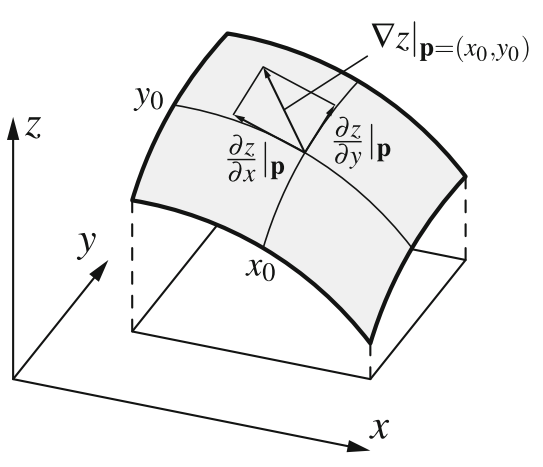
\includegraphics[scale=0.5]{images/gradienmt.png}
    \caption{Intuitive interpretation of the gradient of a real-valued function $z=f(x,y)$ at
        a point $(x_0,y_0)$}
    \label{fig:err_surface}
\end{figure}
Considering this error surface (figure \ref{fig:err_surface}), if we are in the
central point we can look to the derivatives of the error function in the two directions,
the \textbf{gradient} $\nabla$ is the vector tangent to the surface and will tell us the direction where
the surface is more or less increasing.
\newline\newline
If we want to find the solution for our learning we need to look for the minimum of this
error function, so actually we need to look to the opposite direction to the gradient and we
look to reach the minimum.
$$e=\sum_{l\in L_{fixed}}e^{(l)} =\sum_{v\in U_{out}} e_v=\sum_{l\in L_{fixed}}\sum_{v\in U_{out}}e_v^{(l)}$$
So we need to evaluate the gradient to find the direction of the decreasing value, and
we need to go in the proper direction in order to reduce the error. In the case of the MLP
calculate the gradient means compute the partial derivative of the error function in respect
of the threshold and the weights taken as parameters.
\newline\newline
Given $\vec{w}_u=(-\theta,w_{u_1},...,w_{u_k})$ as the vector of weights of a single layer
extended with the threshold, then compute the gradient as follow:
$$\vec{\nabla}_{\vec{w}u}e=\frac{\partial e}{\partial\vec{w}_u}=\left(-\frac{\partial e}{\partial\theta_u},\frac{\partial e}{\partial w_{up1}},...,\frac{\partial e}{\partial w_{up_n}}\right)$$
Since the total error $e$ is given by the sum of the individual errors in respect to all
neurons and all training patterns $l$, we get that:
$$\vec{\nabla}_{\vec{w}_u} e=\frac{\partial e}{\partial\vec{w}_u}\sum_{l\in L_{fixed}}e^{(l)}=\sum_{l\in L_{fixed}}\frac{\partial e^{(l)}}{\partial\vec{w}_u}$$
\begin{figure}[H]
    \centering
    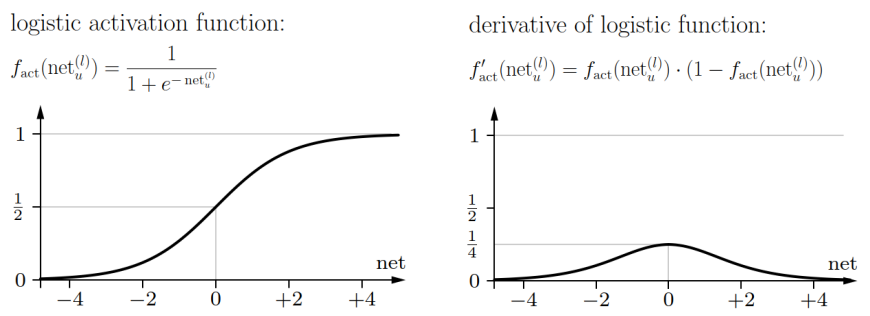
\includegraphics[scale=0.5]{images/logistic_gradient.png}
    \caption{Logistic function as activation function}
    \label{fig:log_func_gradient}
\end{figure}
If we have a \textbf{logistic function} as $f_{(act)}$ we will have that the changes
performed on the vector $\vec{w}_u$ will be proportional to the derivative of the $f_{(act)}$.
More near to $0$ the value of the function will be, more precipitous will be the learning.

\noindent\textit{How we can compute the necessary adjustment for each
    neurons-weight and threshold after we found the error?}
\newline
The process that allow this is called \textbf{error backpropagation}:
\begin{figure}[H]
    \centering
    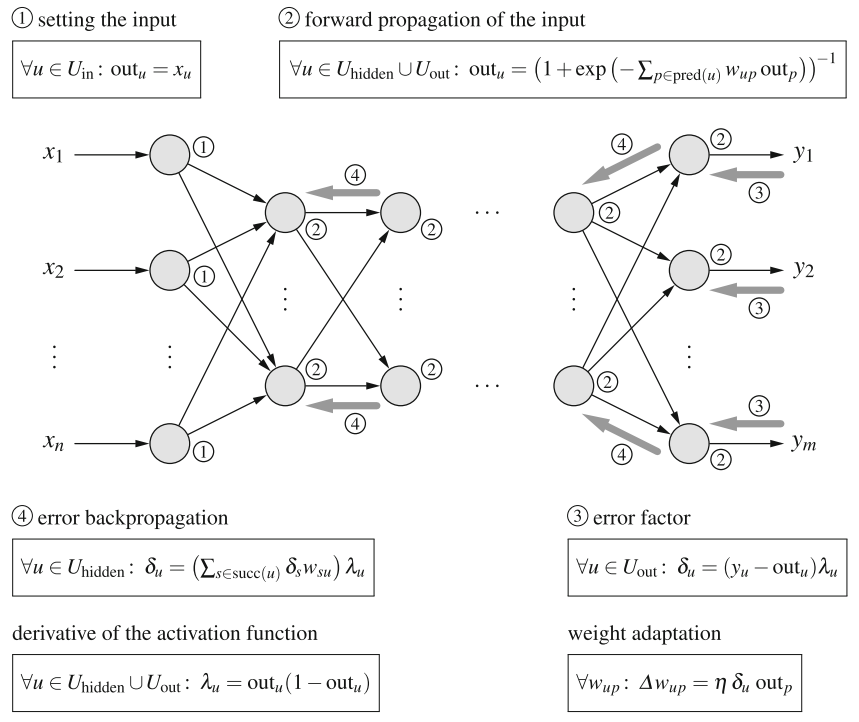
\includegraphics[scale=0.5]{images/error_backpropagation.png}
    \caption{Schematized structure of the error backpropagation process}
    \label{fig:error_backpropagation}
\end{figure}

We assume that the activation functions is a \textit{logistic function} for each neuron
$u\in U_{(hidden)}\cup U_{(out)}$, except for the input neurons.
\begin{enumerate}
    \item Apply the input at the input neurons that is returned without modifications
          at the subsequent first hidden layer.
    \item We compute for each neuron of the subsequent layers the weighted sum of the
          inputs and we apply at the result the logistic function, producing the output
          that will be propagated in all the network until the terminal neurons.
    \item Compute the difference between the desired output and the actual output. since
          it is possible to invert the logistic function $f_{(act)}$, we can know which was
          the input (error) that has induced that particular error ($\delta_u$).
    \item Now that we have transformed the error of the output variable $out_u$ in
          the error of the input variable $net_u$, we can distribute the error (with the correction)
          in a proportional way back to previous neuron, we back propagate the error until the
          input neurons.
\end{enumerate}
We have to say that given the shape of the logistic function the error can disappear
completely, since the gradient will approximate more the \textbf{null vector} the
more it will be near the zero.
\newline\newline
The weight adaptation is performed by the following formula (this tells me how to perform the correction):
$$\forall w_{up}:\delta w_{up}=\eta \delta_u out_p$$
If you initialize the \textit{learning rate} $\eta$ with a too high value instead
of descending the curve we risk to jump from a \textit{"peak"} of the function to another,
without ever converging to the minimum. Furthermore, it is not all certain that the minimum
reached in this way is the global minimum of the function.
\newline\newline
A solution to the problem could consist in \textit{repeating} the learning, initializing
the system with a different configuration of weights and threshold, and then choice
at the end which configuration result in the better minimum.
\paragraph{Negation example}
For example let's consider the negation $\lnot x$, there is a two-layer perceptron for this function.
\begin{figure}[H]
    \centering
    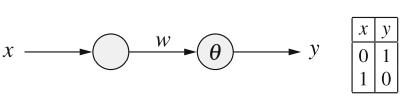
\includegraphics[scale=0.5]{images/2_per_neg.png}
    \caption{Two-layer perceptron with single input and training examples for the negation}
\end{figure}
\begin{figure}[H]
    \centering
    \includegraphics[scale=0.55]{images/squared_errors.png}
    \caption{Squared errors for computing the negation by using a logic activation function}
\end{figure}
From a numeric point of view, this procedure won't allow us to reach really the minimum, we will ahave some
residual errors due to the computation of the various parameters (this will change according to the
process we are adopting).

\subsubsection{Variant of Gradient Descend}
The variant aim to change the \textbf{learning rate} and the \textbf{length of the learning step}.
\begin{itemize}
    \item \textit{Manhattan training}, taking just the sign of the gradient, very fast but you may not reach
          the optimum.

    \item \textit{Flat spot elimination}, it tries to limit the culling of the step length when we get near a
          function plateau by "lifting" artificially the derivative of the function in that point.

    \item \textit{Momentum term}, at each successive step we add to the gradient a fraction of the previous
          with changed weights, so that we can have a sort of memory of how fast it changes respect to the past.

    \item \textit{Self-adaptive error backpropagation}, I allow to each parameter to have a different
          learning rate, in this way we can have a grain fine control respect to the characteristic of the single parameter.

    \item \textit{Resilient error backpropagation}, it's a combination of the Manhattan variation with the Self-adaptive.

    \item \textit{Quick propagation}, instead of using the gradient I approximate the function with a parable and i
          jump directly to the peak of this one.

    \item \textit{Weight decay}, reduces the weights for avoiding to remain trapped in an already saturated region
          (avoiding too big weights to keep stuck neurons).
\end{itemize}

\subsection{Number of hidden neurons}
For a single hidden layer the following rule of thumb is popular (take as granted):
$$\text{Number of hidden neurons} = \left(\frac{\text{number of inputs}+\text{number of outputs}}{2}\right)$$
The problem is that if we have to few neurons in the hidden layer, we will not be able to achieve a good approximation
the function that we need to approximate. We have not enough parameters, this behavior is called \textbf{underfitting}.
\newline\newline
On the contrary, if we have very large hidden layers we have many neurons, we have many many parameters to train and this may force the
NN to learn the examples to much, and this will focus the network on this examples only, we lose the ability of
generalizing the desired behavior, this is called \textbf{overfitting}.
\begin{figure}[H]
    \centering
    \includegraphics[scale=0.6]{images/overfitting.png}
    \caption{The blue curve fits the data points perfectly, not a good model}
\end{figure}
For example, the NN learned perfectly the blue line to pass exactly in the points, but this is not what we
want to have. Now we can't generalize the abstract view of the black line (too many parameters).
\newline\newline
\textit{What we need to do in order to understand when we have good quality for our learning?} Follow, the
next subsection.
\subsection{Cross validation}
In order to understand if we have a good quality for our learning we need to
randomly split our data sets in two parts:
\begin{itemize}
    \item \textbf{Training set}: used for the training.
    \item \textbf{Validation set}: used for checking the quality of the result.
\end{itemize}
This will allow us to see (by using the validation set) if the training makes the NN overfitting the configuration or
not, if the error that we have is still reasonable low, we have a good quality of the learning
(we still can do good generalization), viceversa we have a bad learning quality.
\newline\newline
We can do the splitting in two ways:
\begin{itemize}
    \item \textbf{Cross validation}: splits randomly the data in two subsets (for training and validation),
          we train the MLP with different numbers of hidden neurons on the training data and evaluate them on the
          validation data. Then you repeat the split of the data and the training-evaluation many times and average the
          results. At the end you choose the number of hidden neurons with the best average error.

    \item \textbf{k-fold cross validation}: the data is split in $k$ subsets (called \textit{folds}) of
          equal size. Out of these
          $k$ data subsets, $k$ pairs of training and validation data set are formed by using $1$ fold as a validation
          and $k-1$ folds for training. In this way we train the model for each one of the $k$ training sets, avoiding
          overfitting problems and asymmetric sampling typical of the classic cross validation. In other words the
          sample is subdivided in group of equal size, one group at time is excluded (this is predicted by using the
          non excluded groups), in order to verify the goodness of the prediction model used.
\end{itemize}
randomly the data in two subsets for training and validation (\textbf{cross validation}) and we can repeat this splitting in different
phases and at the end we can compare the. or we can split the data set in N-folds (\textbf{N-folds validation})
and then use the various $n$ subsets for training and $n-1$ subsets for validation, in this way we can use
most of the example for training instead of validation.
\newline\newline
The \textbf{stopping criterion} is also very important, we stop the training when the validation
error is sufficient low.

\subsubsection{Sensitivity analysis}
Sensitivity of the NN to the various parameters that we have, the variations that we may have to the
various parameters influences the behavior of our NN. We want understand how muc hthe learning applied to the NN
is really independent from the behavior of the NN.
\newline\newline
This is important to understand how much is generalizable the behavior of our NN.
\newline\newline
This is a problem for MLP, when we perform the learning (supervised or unsupervised), basically we have a
data set presented to the NN and then the learning algorithm adjust the parameters in ordered to find the
desired behavior of the NN.
\newline\newline
In our hands we have an algorithm, but we don't have an understanding of the why the parameter
are configured in this way. We are trying to give an explanation of why a NN is configured in a specific way,
this is actually field of research (we still don't have a rational idea).
\newline\newline
For the sensitivity analysis which is part of this understanding, we want to answer this question: \textit{How much
    the output of each neuron is changing if we change the data set for training}
(still describing the desired behavior)\textit{?}
So essentially, which inputs the output(s) react(s) most sensitively, it hints about which inputs aren't needed
and may be discarded.
\newline\newline
The approach consists in determine the change of ourput relative to the change of input:
$$\forall u\in U_{in}:
    s(u)=\frac{1}{|L_{fixed}|} \sum_{l\in L_{fixed}} \sum_{v\in U_{out}} \frac{\partial out_v^{(l)}}{\partial ext_u^{(l)}}$$

\subsection{Deep learning}
A modern approach to MLP called \textbf{Deep learning}, with MLP we can approximate any continuos integrable
function, but we have in general a pretty large hidden layer. First problem, \textit{what we can do to
    simplify the structure?} The second problem, with MLP we have to know the characteristic of the data which are
relevant to pick the important data to configure the NN.
\newline\newline
It has been experimented that adding $1$ or $2$ more layers helps to have a concise NN but with
the same characteristic of a MLP with a large number of neurons in the hidden layers.
\newline\newline
The deep learning network is basically a MLP, but with a difference: What we want to do it consists
in not having any type of knowledge about the problem and try to force the NN to configure itself with
a limited and small number of neurons.
\newline\newline
For example, let's consider the $n$-bit parity function, which output $1$ if the $n$-bit word is even,
or viceversa $0$. If we want to use an MLP with only one hidden layer, which has $2^{n-1}$ neurons, the number
of hidden neurons grows \textbf{exponentially} with the number of inputs. This because the function is a
disjunction of  $2^{n-1}$ conjunctions.
\begin{figure}[H]
    \centering
    \includegraphics[scale=0.5]{images/nbit_parity.png}
    \caption{$n$-bit parity function}
\end{figure}
Instead if we use \textbf{multiple} hidden layers, the \textbf{linear growth} is possible (respect to the
input). This finding bring to the developing of \textit{deep learning}, where the \textit{"depth"} is the
one given by the longest path which separates the input neurons from the output neurons.
\newline\newline
The rational is to allow a greater deepness of the network in change of better performance in construction
and computation of the NN. The deep learning bring some downsides:
\begin{itemize}
    \item \textit{Overfitting}: the increases of neurons given from the extra hidden layers can multiply
          the parameters in a disproportional way.
    \item \textit{Vanishing gradient}: during the propagation of the error the gradient will get reduced
          until the vanishing.
\end{itemize}
Some solutions to the overfitting issue:
\begin{itemize}
    \item \textit{Weight decay}: set a maximum limit to the values which can assume weights
          this for preventing an adjustment too much dependent from the data set.
    \item \textit{Sparsity constraint}: introducing some limit to the number of neurons of the
          hidden layers, or limiting the number of the active neurons.
    \item \textit{Dropout training}: some neurons of the hidden layers are omtitted during the
          evolution of the network.
\end{itemize}
While the issue of the vanishing gradient is given by the fact that the activation function it's a
logistic function, which derivative reach at max the value of $\frac{1}{4}$. As consequence of this
the propagation of the error to a previous layer adds a value, often smaller than $1$, and in this
way reducing the gradient.
\newline\newline
A solution consists in editing slightly the activation function in a way that will be always increasing.
Some candidates for that are the \textit{ramp function} and the \textit{softplus function}.
\begin{figure}
    \centering
    \includegraphics[scale=0.5]{images/ramp_softplus.png}
    \caption{Ramp function and softplus function}
\end{figure}
A totally different approach consist in building the network \textit{"layer by layer"}. A much used
technique consists in think at the NN like a stack of \textit{autoencoder}. An autoencoder is an MLP
which maps the input inside an approximation, using an hidden layers of less dimensions. The
hidden layer works like an \textit{encoder} by encoding the input in a internal representation
which will be decoded to the output layer. The autoencoder, has only one layer, it doesn't suffer
about the same limitation and can be traversed normally from the backpropagation.
\newline\newline
A problem with this approach is that if there are a lot of neurons in hidden layer as much are in
the input layer we are going to propagate with less adjustments, and without the autoencoder
extracting any knowledge from the data.
\newline\newline
There are three possible solutions:
\begin{itemize}
    \item \textit{Sparse autoencoder}: provide to use a much smaller number of neurons inside the
          hidden layers, respect to the input layers. The autoencoder will be forced to extract from
          the input some features instead of just propagating the data.

    \item \textit{Sparse activation scheme}: in a similar way for avoiding the overfitting, we
          decide to \textit{"shutdown"} some neurons during the computation.

    \item \textit{De-noising autoencoder}: we add randomly some noise to the input.
\end{itemize}
For obtaining an MLP with multiple layers we combine differente autoencoder. Initially we start by
training just one autoencoder. At that time you remove the decoder and you preserve only the internal layer.
You use the data processed from this autoencoder for training the second, and so on until you
reach a satisfiable number of layers.
\begin{figure}
    \centering
    \includegraphics[scale=0.5]{images/autoencoder_decoder.png}
    \caption{Autoencoder and autoencoder with the decoder removed}
\end{figure}
MLP constructed in this way are really efficient at recognizing with success hand written numbers. If
we would want to use similar NN for a more broad class of applications, like, for example, the
feature recognized by the internal layers are not located in a specific portion of the image, we would
need to use a CNN (\textit{Convolutional Neural Network}, next topic). This architecture is inspired
by the working of the human retina, where the neurons used for the perception has a receptive field,
or in other words, a limited region where they can answer to stimulus.
\newline\newline
This is simulated inside the CNN by connecting the neurons of the first layer just to some neurons
of the input. The weights are partitioned in a way that partial networks can be evaluated  from
different prospective of the image.
\newline\newline
During the computation it will proceed by moving the receptive field on the totality of the image. As
result you will obtain a convolution of the weight matrix with the input image.

\subsection{Radial Basis Function Networks}
This is another NN model, we have a special type of structure for the neurons and a special approach
for information we are collecting from images (typically).
\newline\newline
I have a 3-layered feed forward network, where the activation function of the hidden layer is a \textit{
    Radial Basis Function} (RBF).
\newline\newline
An RBF is a function which try to point out what is relevant in a very specific area of the information
we are observing (an image), and tries to diminish what is in the surrounding area. So it will focus on
relevant part of the image where we want to understand the contents.
\newline\newline
In this kind of NN we have a set of values for various inputs, we represent this with a vector, we have
for example a three dimensional space, where each value represent the input. What I'm considering as input
of the hidden layer is the difference between this vector and the weight vector, which is the distance
between the vectors.
\begin{figure}[H]
    \centering
    \includegraphics[scale=0.5]{images/rbf.png}
    \caption{Distance between $\vec{w}$ and $\vec{in}_{u}$}
\end{figure}
There are different families of distances, we typical consider the \textbf{Minkowski Family}, which are
distances defined in general by this formula:
$$d_k(\vec{x},\vec{y})=\left(\sum_{i=1}^n |x_i-y_i|^k\right)^{\frac{1}{k}}$$
\begin{itemize}
    \item $k=1$: Manhattan distance.
    \item $k=2$: Euclidean distance.
    \item $k\rightarrow\infty$: Maximum distance.
\end{itemize}
\begin{figure}[H]
    \centering
    \includegraphics[scale=0.5]{images/mknowski.png}
    \caption{Manhattan, Euclidean and Maximum}
\end{figure}
The RBF has an activation function in the output layer which is \textbf{linear}. Differently, the
hidden layer has an activation function which is a \textbf{radial function}. A radial function
decreases from $0$ to $\infty$ in a monotonically way.

$$f:\mathbb{R}_0^+\rightarrow[0,1]\text{ with }f(0)=1\text{ and }\lim_{x\rightarrow\infty}f(x)=0$$
The size of the \textit{catchment region} of the function is defined by
the \textbf{reference radius} $\sigma$, the bigger is the $\sigma$ the bigger
is the area observed by the neuron. The various parameters and the shape of the function
determine the width of this radius. The radial activation function are typically shaped in this way:
\begin{figure}[H]
    \centering
    \includegraphics[scale=0.4]{images/radial_functions.png}
    \caption{Radial activation functions}
\end{figure}
As example, let's apply an RBFN for simulating the boolean conjunction $x_1\land x_2$.
When I'm around the black point, the input is $(1,1)$, what we want to do is creating a circle
around that area where the output is $1$ (significant information to extract).
\newline\newline
Another approach could consist in considering a RBF in the opposite way, where the interesting
data is outside the circle.
\begin{figure}[H]
    \centering
    \includegraphics[scale=0.5]{images/RBFN.png}
    \caption{RBFN for conjunction}
\end{figure}
Another example is with the bi-implication $x_1\longleftrightarrow x_2$:
\begin{figure}[H]
    \centering
    \includegraphics[scale=0.4]{images/RBFN_bi.png}
    \caption{RBFN for bi-implication}
\end{figure}

\paragraph{Function approximation}
We have two neurons focusing on the relevant part of the domain, the rest will be $0$, and by merging
this two information you will get the bi-implication. In general an RBFN as the same expressive
power of an MLP, and it can be saw as an universal approximator (can approximate any Riemann integrable
function) with a small arbitrary error.
\newline\newline
The process is the same of the other NN, the function will get approximated with a step function that
can be computed easily by a RBF if we define that as the weighted sum of rectangular functions.
\begin{figure}[H]
    \centering
    \includegraphics[scale=0.4]{images/scale_func.png}
\end{figure}
Each pulse can be represented by a neuron of a RBFN:
\begin{figure}
    \centering
    \includegraphics[scale=0.5]{images/nn_funcapprox_rbfn.png}
    \caption{RBFN for the approximation, using the step function}
\end{figure}
The approximation can be enhanced by increasing the number of points where the function is
being evaluated. Furthermore, if instead of using the rectangular function, we
use the Gaussian we obtain more "soft" transitions, avoiding big jumps (like for the MLP).
\begin{figure}[H]
    \centering
    \includegraphics[scale=0.4]{images/gaussian_rbfn.png}
    \caption{RBFN for the approximation, using the Gaussian function}
\end{figure}

\subsection{Training RBFN}
We want to apply in principle a sort of backpropagation in order to perform the configuration,
like with the FFN.
The principle is always the same, having in mind the \textit{minimization} of the final error,
but the problem here is \textit{how we can decline this by taking into account the
    specific structure of this neurons?}
With the others ANN the initialization phase was trivial, because you just had to
select some random values, instead with RBFN the same approach conduce to suboptimal
results.
\newline\newline
Let's consider a \textbf{simple radial basis function network}, which is
a partial view of the general structure of a RBFN, where each training example is associated
with a proper radial function.
\newline\newline
We want to apply a \textbf{fixed learning task} $L_{fixed} = \{l_1,...,l_m\}$ with
$m$ training patterns $l=(\vec{l}^{(l)},\vec{o}^{(l)})$ composed by input and desired outputs.
\newline\newline
We have one hidden neuron $v_k, k=1,...,m$ for each training pattern, let's define the vector
of associated weights to the neuron $v_k$:
$$\forall k\in\{1,...,m\}\vec{w}_{v_k}=\vec{i}^{l_k}$$
Let's consider the activation function of our neuron equal to the sigma specific to that
neuron, the radius can be computed for each of the neuron by considering heuristic approach
in which we take the distance between the various input patterns and we take the maximum
distance computed between each pair of input vectors (patterns) in our dataset (this value
is expressed as $d_{max}$).
\newline\newline
The radius of the neuron $\sigma_k$ will be choose heuristically if the activation
function is Gaussian function:
$$\forall k\in\{1,...,m\}:\sigma_k = \frac{d_{max}}{\sqrt{2m}}$$
$$d_{max}=max\underset{l_j,l_k\in L_{fixed}}{d\left(\vec{l}^{(l_j)},\vec{l}^(l_k)\right)}$$
Where $d_{max}$ is the maximum distance between the input vectors.
This choice allow to center the various Gaussians in such a way that them doesn't overlap each other,
instead they will distributes in an ordered way respect to the input space.
Basically we have a structure where we try to learn with each neuron one of the input patterns,
one neuron trying to well understanding a specific input pattern.
\linebreak\\\noindent I can initialize the connections from the hidden to the output
neurons by using weights, this can be done by considering this formula:
$$\forall u:\sum_{k=1}^{m}w_{{u_v}_m} out_{v_m}^{(l)}-\theta_u=o_u^{(l)}$$
which is the weighted summation of the output of the hidden layer and considering the threshold
of the output, which has to be equal to the \textbf{desired output}. We know the desired output,
we have the threshold and the current output generate by the hidden layer, so the last thing we
need is the weights, this can be obtained by multiplying the interconnections weight by the
matrix $A$ of the output of the hidden layer (by using $\theta=0$):
$$\textbf{A}\cdot\vec{w}_u=\vec{o}_u$$
Where $\textbf{A}$ is the $m\times m$ matrix that has for components the various output of the
neurons in the hidden layer. If the matrix $\textbf{A}$ has the complete rank, we can invert that and
compute the weight vector:
$$\vec{w}_u=\textbf{A}^{-1}\cdot\vec{o}_u$$
This method guarantee a perfect approximation. This means that is not necessary training
a simple radial basis function network. In general, if we don't want to have for each pattern a neuron,
we will have to select $k$ subsets from the dataset and find, for each subset, a representative che assoceremo
to a neuron in the hidden layer.
\begin{figure}
    \centering
    \includegraphics[scale=0.4]{images/example_biimp_rbfn.png}
    \caption{Example of the computing the weight vector in the bi-implication problem}
\end{figure}
if we look graphically, for each of the hidden layer we have aRBFN shaped as a Gaussian,
which will correspond at each example that the neurons will learn. We will have only
two of this Gaussian in the final computation, we will generate an output that will
have to be different from $0$. This is a RBFN centered in the relevant example that
we want to learn.
\begin{figure}
    \centering
    \includegraphics[scale=0.4]{images/rbfn_gauss.png}
    \caption{RBFN function centered in the examples}
\end{figure}
This is not the general case, if we take a structure like this and we want to create
a RBFN having in mind that for each the pattens we have to contribute we need to put a neuron
with RBFN as activation function, this implies that if we have many examples that we want to learn
we are going to have an incredibile big structure for our network, and this is not smart.
\newline\newline
If we are considering the general radial basis function structure in which we don't want to have a neuron with $x$
RBFN network centered on a specific example to learn, we need to try to limit the number of neurons
we need to understand which are the neurons which are relevant and understand where to place it.
Basically we need to select among the $m$ patterns that we want to learn a subset of $k$ patterns
adn then we need to put the neuron centered on this example, then we need to figure out how to build
the other outputs by combining this limited number of examples that we learn.
\newline\newline
If we want to use this kind of approach we basically need to understand were to place the center,
but we need also to understand how large will be the radius in order to be sure that
after placing the Gaussians we are able to recreate the examples for which we don't use the
Gaussian.
\newline\newline
What I can do is splitting the domain of examples, and then for each subdomain find a representative
point (not an example) in the subdomain, that will cover the group of the examples (not points)
of the subset.
\newline\newline
This can be formalized in saying that we select $k$ training patterns as centers, where
the connection weights for the hidden neurons are the training pattern, and the connection
weights for the output neurons can be obtained by considering this matrix $A$:
\begin{figure}[H]
    \centering
    \includegraphics[scale=0.4]{images/matrix_conn_weights_rbfn.png}
    \caption{Matrix that expresses the connections weights for output neurons}
\end{figure}
Now I can apply the invert the matrix for computing the weights since system over-determined (not
squared), but I can consider the pseudo inverse matrix:
$$A^+=(A^T A)^{-1} A^T$$
Now we can apply the actual computation for our vector $\vec{w}$ of the weights, given by:
$$\vec{w}_u = A^+\vec{o}_u$$
So now, \textit{how we can choose the center for creating the configuration for our RBFN?} As
for the simple case we can take all points we just need to determine the radius for one single
radius and the output weights (considering that we want to use a better structure, which is
practicable).\\Options of radial basis function centers:
\begin{itemize}
    \item All data points as centers, the simple case where only radius
          and output weights need to be determined. The output values
          ca be achieved exactly, computing the weights is unfeasible.
    \item Random subset, this is fast, only radius and output weights need to be
          determined. The performance depends on the choice of data points.
    \item Clustering, c-means clustering (the centroid point representative for the
          examples in the subset).
\end{itemize}

\subsubsection{C-means clustering}
This is one of the best options for choosing the RBFN centers:
\begin{enumerate}
    \item Considering a number of $c$ clusters to be found (input).
    \item Initialize the cluster centers \textbf{randomly}.
    \item Assign initially the data points (the examples) to the nearest center (or \textit{centroid}).
    \item Adjusting the position of the center considering the position of the assigned data points (mean
          vectors of the assigned data points, this is called \textbf{cluster center update}).
    \item Repeat the step $3$ and $4$ until clusters do not move anymore (converge).
\end{enumerate}
\begin{figure}[H]
    \centering
    \includegraphics[scale=0.4]{images/c-means.png}
    \caption{Step $1$ with $c=3$, Step $2$ randomly choosing the centroids}
\end{figure}
Then by using the \textbf{Delaunay Triangulation} of the centroids, which leads
to the \textbf{Voronoi Diagram} by taking the line orthogonal to each one of the three
edges. This will result in a tessellation of the domain of the function, basically
each tassel of the domain is a cluster.
\begin{figure}[H]
    \centering
    \includegraphics[scale=0.4]{images/c-means1.png}
    \caption{Delunay Trianglulation (left) and Voronoi Diagram (right)}
\end{figure}
After that I'm going to search for the new centroid of each cluster, where the sum of the
distances is minimal, after finding this element I will consider it as the new center.
Then I will apply again the same partition (Delunay-Voronoi) as before.
\begin{figure}[H]
    \centering
    \includegraphics[scale=0.4]{images/c-means2.png}
    \caption{Centroid update}
\end{figure}

\pagebreak
\subsection{Learning Vector Quantization}
\textit{What happen if we don't have examples with a desired output (only the examples)?}\\Basically,
until now we saw the fixed-learning task, now we want to see what happens with a free-learning task.
\newline\newline
Now I'm going for searching outputs that will be similar to the given input.
\newline\newline
We still consider the Delaunay and Voronoi approaches.
The problem is that what we want to do is a suitable quantization of the domain in which
we have our examples in order to understand the group of the examples which are similar.
In the previous example we had given a number of clusters, now we want to find the clusters
in a given dataset.
\newline\newline
Let's considered the input examples (or data points) as empty circles, and the cluster centers
(or points) by the full circles.
\begin{figure}[H]
    \centering
    \includegraphics[scale=0.5]{images/vector_quant.png}
    \caption{Vector quantization}
\end{figure}
The \textbf{Learning Vector Quantization Network} (LVQ/LVQN), is a FFNN with 2-layers that performs this clustering
of the examples by similarity, basically from an abstract point of view we see the LVQN as a RBFN in which the hidden layer and output layer are collapsed in a single layer.
\newline\newline
The network input function of each output neuron is the distance between the input vector and the
weight vector. The definition of the distance is the same, we are considering the Mynkowski family
and the euclidean distance for represent the behavior of our function,
\newline\newline
The output activation function of each neuron is not a simple function of the activation of the
neuron: it considers the activation of \textbf{all} output neurons.
\begin{figure}[H]
    \centering
    \includegraphics[scale=0.4]{images/act_lvqnn.png}
\end{figure}
We don't just look locally, for example with $4$ neurons we will look to the value of the activation
in the activation function of each neuron and we compare the activation value of each on of them. The
biggest activation value will lead to an output $1$ otherwise $0$ (when the activation is smaller). We
have one neuron winning over all the other, basically we have a connection between all neurons in the
output layer such that each of them is looking to what the other neurons are doing (the activation),
this will allow the confrontation.
\begin{figure}[H]
    \centering
    \includegraphics[scale=0.6]{images/lvqq_neur_confront.png}
\end{figure}
In the LVQN we can use the same radial functions that are use for any RBFN.
\newline\newline
\textit{How can we perform the configuration ?}
Basically for each training pattern we look to the \textit{reference vector} which is
we find the closest reference vector.
\newline\newline
I may have basically two strategy that I can consider in order to perform the adjustment of the
weights:
\begin{itemize}
    \item \textbf{Attraction rule}, when the data point and the reference vector have same
          class:
          $$\vec{r}^{(new)}=\vec{r}^{(old)}+\eta(\vec{x}-\vec{r}^{(old)})$$
    \item \textbf{Repulsione rule}, when the data point and the reference vector have different
          class:
          $$\vec{r}^{(new)}=\vec{r}^{(old)}-\eta(\vec{x}-\vec{r}^{(old)})$$
\end{itemize}
where $x$ is the input, $r$ is the reference vector for the winner neuron, and $\eta$ is the learning
rate. Until now we meant the learning rate as fixed during the learning, by the way the are some
situations were the constant learning rate can bring some problems.
\begin{figure}[H]
    \centering
    \includegraphics[scale=0.4]{images/adapt_rulesa.png}
    \caption{Adaptation rules applied on the reference vector}
\end{figure}
In the case of the attraction rule we move the reference vector $\eta d$ towards $x$
which is the same class of the reference vector. Or in the right diagram where
we are moving the reference far from the reference $x$ so that that the element
moves to another class.
\begin{figure}[H]
    \centering
    \includegraphics[scale=0.5]{images/onlk_batch_adap.png}
    \caption{Adaptation rules in case of online and batch learning}
\end{figure}
In the case of the online training we have a step each time according to the various
pattern I'm presenting, in the batch training I apply the various
connection for the group of examples belonging to the same pattern and perform the update at the end
of an epoch (the solution of the position of the centers is smoother
since I am putting together more then one example).
\begin{figure}[H]
    \centering
    \includegraphics[scale=0.5]{images/time_dep_lm.png}
    \caption{Fixed learning rate to time dependent learning rate}
    \label{fig:tdln}
\end{figure}
The problem I have with this kind of techniques, is that if I consider a fixed learning rate,
which is a coefficient which tells me how much I want to change the position by taking
into account the similarity.
\newline\newline
I may enter in a oscillation (left diagram), in this case
what we can do is to dynamically change the learning rate consists by decreasing it
as it grows iterations (called \textbf{time dependent learning rate}, \ref{fig:tdln} on right).
\newline\newline
There are some applications in which I may have some more information
about the data tha I have, \textbf{classified data}, I may have some more information
related to the class to which an example belong and even
if I'm not using the supervised learning I can take advantage of this information
so that I can update not only the reference vector but I can consider updating also
some other reference vector the once which are the nearest the reference vector
that I'm considering.
\newline\newline
The problem is that this may move the classes very far one from the other,
one option to balance this is to consider the \textit{window rule}: a reference vector will become adapted
only if the point $p$ is near the border of the classification, the hyper-surface which separates
the contiguous regions of the two classes. The notion of closeness is formalized as :
$$min\left(\frac{d(\vec{p},\vec{r}_)}{d(\vec{x},\vec{r}_k)},\frac{d(\vec{x},\vec{r}_k)}{d(\vec{x},\vec{r}_j)}\right) > \theta
    \text{ where } \theta=\frac{1-\xi}{1+\xi}$$
where $\xi$ is a parameter specified from the user, which describes the "amplitude" of the window
around the border of the classifications. If we assume that the data are randomly chosen from
a random set of normal distributions, we could use a \textit{soft} approach, in opposite to a "crisp"
division typical of the clustering like the \textit{c-means}. Basically we don't have a RB function
which is rather sharp but I'm considering a smooth border between the classes induced by
sufficiently large RBF. In this cases I can considering the classing by a mixture og
Gaussian which are representing the various classe, with a softer border between
the various classes.
\newline\newline
In order to do this I have to consider that each element is not interbelonging
to one class or another, each element of my data set as a probability of belonging to one or the other class.
This is due to the fact that I have a gaussian shape of the radial basis function,
In this case what I will do is essentially to evaluate the probability for each example to
belong ot each of the classes introduced in my system. Formal definition:
\begin{figure}[H]
    \centering
    \includegraphics[scale=0.4]{images/formal_prob_func.png}
    \caption{Probability function}
\end{figure}
If I take the various examples of my dataset I have a set of clusters in my dataset with the parameter that defines
the cluster, and for each element of the dataset I want to understand the prbability of belonging to
one class respect to another.
\newline\newline
Mathematically this is very complex to be optimized, and as a consequence we try to perform an approximation introducing
in an explicit way the position of the various Gaussians with additional random variables which are difficult to
compute it in a exact way, we compute a maximum expected value for that, and we try to get the
maximum of the likelihood.
\newline\newline
Basically what we need to do to perform the maximization of the likelihood, we work in two passes since we have the centers,
and the distribution of our variables, what we can do basically we optimize the initial group
of centers of the clusters and after this we can compute the maximum likelihood on the data we have.
The what we do we do maximization.
\begin{enumerate}
    \item Computing the center
    \item Computing the normal distribution
\end{enumerate}
The final result will be an approximate value of the density function, of belonging to each
specified class for each data that we have in the data set. We will have a softer definition of
the border but this will bring a much more complex analysis.

\subsection{Self-organizing maps}
Sometimes are called also \textit{Kohonen maps}, introduce from the Prof. Kohonen. It is a two-layer
FFNN similar to the VQLN, instead of having in the output layer all the other output neurons, the
self-organizing map has local connections only among neighboring hidden/output neurons.
\newline\newline
We do not have the winner take all over the entire set of output neurons but we work local, this is applied
on the neighbor of each neuron. The network input function is the radial function,as before, the
\begin{figure}[H]
    \centering
    \includegraphics[scale=0.5]{images/som_examp.png}
    \caption{Example of neighbor connections for each neuron}
\end{figure}
By the way in SOM the neighbor are defined in a bi-dimensional space:
\begin{figure}[H]
    \centering
    \includegraphics[scale=0.6]{images/som_bi.png}
    \caption{Neurons expressed as squared or hexagonal grid}
\end{figure}
the black ones are representing the neurons, where the surrounding square (or hexagon)
of a neuron is the neighbor. The grey lines represents the regions assigned to a neuron.
\begin{figure}[H]
    \centering
    \includegraphics[scale=0.5]{images/topology_sop.png}
    \caption{The topology is preserved}
\end{figure}
basically in this kind of structure we want to analyze the data and we want to have a winner
for each data, but what we want also is to to preserve the neighborhood, so the topology
of the structure.
\begin{figure}[H]
    \centering
    \includegraphics[scale=0.5]{images/neigh_asoc_topo.png}
    \caption{The neuron space (2D grid) and the input space (3D grid)}
\end{figure}
Basically what we want to do in this kind of network is how we associate the element of the dataset with the neuron
in my grid preserving the similarity and the concept of neighboring saw before. This is how we can update
parameter of our network, and enforcing the parameters of the winning neuron:
$$\vec{r}_u^{(new)} = \vec{r}_u^{(old)} + \eta(t) f_{nb} (d_{\text{neurons}} (u,u_*), \rho (t)) (\vec{x}-\vec{r}_u^{(old)})$$
in time I will reduce the learning radius , so I can focus the capacity of learning a specific pattern
this will allow me to create a much stronger partitioning in classes by similarity.
Considering a neighboring function with is smooth, I may consider a smooth border and an example may excide more t***
\newline\newline
The training will work by placing the elements randomly and adjust the interconnection by adjusting the winning neuron***
\newline\newline
Example a grid 10 by 10
random associations of hte network, each step will associate with the similar example.
another example,
the problem is always the same the initial configuration is poor and the NN can't flatten the configuration
of the grid. Maybe the neighbor radius is too small or le the learning rate is too small.
\newline\newline
Basically starting from the original 3D we are able to flat in a bi-dimensional one. This can be used for reduce the
bi-dimensionality of the dataset

\subsection{Hopfield Networks}
The Hopfield Network (HN) is an ANN with a loop in the graph. We have not seen in practice
what happens with a loop that feed back the information. Is the simplest type of
\textbf{recurrent network}, a graph with direct cycles. A first difference of HN in respect to the other ANN is
that all the neurons are both input that output. There is no hidden layer of neurons, each neuron is connected
to another (except single neuron loops) and the connection weights are distributed symmetrically.

\paragraph{Definition}\mbox{}\\
An Hopfield network is a neural network with a graph $G=(U,C)$ that satisfies the following conditions:
\begin{enumerate}
    \item $U_{hidden}=\emptyset, U_{in}=U_{out}=U$
    \item $C=U\times U-\{(u,u)|u\in U\}$
\end{enumerate}
The connection weights are symmetric, $\forall u,v\in U, u\neq v: w_{uv}=w_{vu}$. The network input
function of each neuron $u$ is the weighted sum of the outputs of all other neurons:
$$\forall u\in U: f_{net}^{(u)}(\vec{w}_u,in_u)=\vec{w}_u in_u=\sum_{v\in U-\{u\}}w_{uv}out_v$$
The activation function of each neuron $u$ is a threshold function
\[
\forall u\in U: f_{act}^{(u)}(net_u,\theta_u)=
\begin{cases}
    1&\text{if }net_u\geq 0\\
    -1&\text{otherwise}
\end{cases}
\]
The output function of each neurons is the identity, that is,
$$\forall u\in U: f_{out}^{(u)}(act_u)=act_u$$
Since the connection weights are symmetric also the matrix will be symmetric
\[
    W=
    \begin{bmatrix}
        0                & w_{u_1u_2}  & \dots  & w_{u_1u_n} \\
        w_{u_1u_2}       & 0           & \dots  & w_{u_2u_n} \\
        \vdots           &\vdots       & \ddots & \vdots \\
        w_{u_1u_n}       & w_{u_2u_n}  & \dots  & 0
    \end{bmatrix}
\]
\paragraph{Simple Example}\mbox{}\\
\begin{figure}[H]
    \centering
    \includegraphics[scale=0.7]{images/simple_hop.png}
    \caption{The HN oscillates if the activations of the two neurons are updated in parallel,
    but reaches a stable state if the neurons are updated alternatingly}
    \label{fig:s_h1}
\end{figure}
\[
    W=
    \begin{bmatrix}
         0 & 1 \\
         1 & 0
    \end{bmatrix}
\]
Essentially what we have is a single layer of neurons for which we have the inputs that are
giving the incoming data to them, they are operating in such a way that the output of the neuron
are feeding the other neurons in the structure.
\newline\newline
The behavior of a Hopfield network can depend on the update order
\begin{itemize}
    \item Computations can \textbf{oscillate} if neurons are updated in parallel (\textbf{synchronous parallel update}, fig.\ref{s_h1}).
    \item Computations always \textbf{converge} if neurons are updated sequentially (\textbf{asynchronous/sequential update}, fig.\ref{s_h1}).
    This is assured by the \textbf{convergence theorem}.
\end{itemize}
\begin{itemize}
    \item This means that we have a single layer of neurons that still have an output arc, they
    can't only send data for feedback.
    Basically this creates a kind of \textbf{memory}, where what is generated in a previous step is reused for the
    subsequent step (by the way this is the motivation for introducing this kind of network).

\item The relevance of the output arc is the same of the feedback arc. the network input function is
    only the weighted summation of the output of all the other neurons.

\item The we will generate the network neuron of the value, this is the input value of the activation
    function, the activation function that we are using is essentially the step function.

\item The output function for this neuron is the identity function. If we want ina concise way represent all
    the connections we can use a matrix for collect all the weights. The diagonals is composed by 0
    because this means that we don't have any contribution to the next neuron. The matrix is symmetric
    so that the interconnection id passed correctly
\end{itemize}
There is the possibility to simplify the representation of more complex HN
\begin{figure}[H]
    \centering
    \includegraphics[scale=0.3]{images/simpliefied_hop.png}
    \caption{Simplified representation of a HN}
    \label{fig:h2}
\end{figure}
Where:
\begin{itemize}
    \item The symmetric connections between neurons are combined.
    \item Inputs and outputs are not explicitly represented.
\end{itemize}
This will enhance the readability of the graph in more complex cases, and allow a more
abstract view of the HN and still exploiting the characteristics of the network.
\subsubsection{State graph}
In order to understand how the computation \textbf{evolves} and how we reach the final ready state we have
to introduce the \textbf{state graph}. It will give the values of the activation and
transition inside the HN. Each node in the graph represent a configuration that we
have foreach neuron. The "+/-" encodes the neuron activations:
\begin{itemize}
    \item The + means that is active.
    \item The - means that is not active.
\end{itemize}
\begin{figure}[H]
    \centering
    \includegraphics[scale=0.5]{images/state_graph.png}
    \caption{State graph of the HN in figure \ref{fig:h2}}
\end{figure}
The arrows are labeled with the neurons, an the updates of which causes the corresponding state transition.
\begin{itemize}
    \item \textbf{Stable states}, cannot be left again (represented in grey).
    \item \textbf{Unstable states}, may be left again (represented in white).
\end{itemize}

\subsubsection{Convergence therem}
It actually possible to prove the convergence theorem which tell us that if I active the HN
in a sequential (\textbf{asynchronously}) way a steady state is reached in a finite number of steps.
\newline\newline
If the neurons are traversed and updated cyclically in
an arbitrary, but fixed order, at most $n\cdot2^n$ steps (updates of individual
neurons) are needed for reach the convergence, where $n$ is the number of neurons of the HN.
\newline\newline
The proof is carried out with the help of an energy function.
Basically to prove this we can rely on the fact the we can associate to the behavior of the network
an energy which can be defined in this way (not actual physical energy), but if you look
to the shape of the function is the typical structure of an energy function:
$$E=-\frac{1}{2}\vec{act}^\top \vec{W}\vec{act}+\vec{\theta}^\top\vec{act}=$$
$$=-\frac{1}{2}\sum_{u,v\in U,u\neq v}w_{uv}act_u act_v+\sum_{u\in U}\theta_u act_u$$
It is important to point out that the order of activation of neurons doesn't matter we will
reach a steady state.
\newline\newline
We can observe that the system can only evolves from one state with higher energy to another
with lower energy. A stable state will be a local minima of the energy function.
\newline\newline
A steady state is reached when no output is changing, if a neuron is changing throughput
the previous state of the graph can't
be reached. To go back to the previous state we need to increase the energy. Any physical system
tries to reduce the total energy in the system. The second problem that forbid the fact of
coming back to the previous state is due to the fact that this implies that we may need
to change two outputs to go back as consequence even if is not the complete parallel of the
neuron ,that we are not following strictly the sequential activation.
\paragraph{Associative memory}\mbox{}\\
We can exploit this theorem for using the HNs as \textbf{associative memories},
this by connecting a data reference to the stable state achieved (after HN computation).
In this way we can use stable states to store patterns: \textbf{Hebbian learning rule}
\begin{enumerate}
    \item Store only one pattern $p$
        \begin{itemize}
            \item Find weights so that pattern is a stable state.
            \item $W=pp^T - E$
            \item $w_{uv}=\begin{cases}0 &u=v\\ 1 & u\neq v,act^{(p)}_u=act^{(p)}_v\\ -1 & otherwise   \end{cases}$
        \end{itemize}
    \item Storing several patterns
        \begin{itemize}
            \item Computer $W_i$ for each pattern $p_i$
            \item $W=\sum_i W_i$
        \end{itemize}
\end{enumerate}
\paragraph{Optimization problems}\mbox{}\\
In the same way we can exploit the HN for solve optimization problems. We use energy minimaztion to
solve the optimization problems.
\begin{itemize}
    \item Transform function to optimize into a function to minimize.
    \item Transform function into the form of an energy function of a HN.
    \item Read the weights and threshold value from the energy function.
    \item Construct the corresponding HN.
    \item Initialize HN randomly and update until convergence.
    \item Read solution from the stable state reached.
    \item Repeat several times and use best solution found.
\end{itemize}

\subsection{Boltzman machines (italian)}
Le macchine di Boltzmann sono un modello di network che sono in relazione stretta con gli
HN. Alcune variazioni speciali di questo modello hanno ottenuto un interesse rilevante
recentemente (specialmente nel Deep Learning). Una macchina di Boltzmann standard differisce
da un HN principalmente nel come gli stati dei neuroni vengono aggiornati (
e per il fatto che può contenere neuroni nascosti)..
\newline\newline
Come per le reti Hopfield per la risoluzione di problemi di ottimizzazione si affidano ad
una \textbf{funzione energetica} che assegna un valore numerico ad ogni stato del network. Con
l'aiuto di questa funzione engergetica viene definita una distribuzione probabilistica su gli
stati del network che è basata sulla \textbf{distribuzione di Boltazmann}:
$$P(\textbf{s})=\frac{1}{c}e^{-\frac{E(\textbf{s})}{kT}}$$
dove il vettore il vettore $\textbf{s}$ descrive lo stato del sistema, $c$ è la costante di
normalizzazione, $E$ è la funzione che restituisce l'energia di uno stato $s$, $T$ è la temperatura
termodinamica del sistema e $k$ è la costante di Boltzmann.
\newline\newline
Per le macchine di Boltzmann il prodotto $kT$ è spesso sostituito solo da $T$, così combinando
la temperatura e la costante di Boltzmann in un singolo parametro. Inoltre, lo stato $s$ consiste
nel vettore $\textbf{act}$ delle attivazioni dei singoli neuroni.
$$E(\textbf{act})=-\frac{1}{2}\textbf{act}^\intercal \textbf{W} \textbf{act}+\theta^T \textbf{act}$$
dove $W$ è la matrice dei pesi connessi e $\theta$ il vettore contenente I valori delle soglie (o threshold).
\newline\newline
Ora guardiamo il singolo neurone $u$ e elaboriamo il cambio energetico che viene portato da
questo neurone durante il suo cambiamento di stato. Consideriamo la differenza assoluta in energia
tra $act_u=0$ e $act_u=1$ (mentre tutti gli altri neuroni mantengono la loro attivazione):
$$\Delta E_u=E_{act_u}=1-E_{act_u}=0=\sum_{v\in U-\{u\}}w_{uv}act_v-\theta_u$$
scrivere l'energia in termini di distribuzione di Boltzmann restituisce:
$$P(act_u=1)=\frac{1}{1+e^{-\frac{\Delta E_u}{kT}}}$$
cio è, la probabilità di un neurone di essere attivo in una funzione logistica della differenza
energetica tra stato attivo ed inattivo. Visto che la differenza energetica è strettamente connessa
al network in input del neurone:
$$\Delta E_u=\sum_{v\in U-\{u\}}w_{uv}act_v-\theta_u=net_u-\theta_u$$
questa formula suggerisce che una procedura con aggiornamento stocastico per il network.
La procedura di aggiornamento sviluppa come segue:
\begin{itemize}
    \item Un neurone $u$ di una data macchina di Boltzmann viene scelto e calcola
          la sua differenza energetica $\Delta E_u$ (attraverso la funzione logistica) e
          con questo la sua probabilità di attivazione.
    \item Questo aggiornamento viene ripetuto tante volte per ogni neurone scelto
          casualmente fino alla convergenza del sistema. La convergenza verso uno stato sstabile
          è garantita dal fatto che latemperatura del sistema non cresce nel tempo, ma diminuisce.
          Ad un certo punto si raggiungerà uno stato stabile, anche detto \textbf{equilibrio termico} (
          thermal equilibrium) del sistemam che rappresenterò un minimo (possibilmente locale)
          della funzione.
\end{itemize}
Questa procedura si chiama \textbf{Markov-Chain Monte Carlo}.
\newline\newline
Bisogna notare che una BM potrà calcolare in modo efficace una distribuzione di probabilità se
gli esempi forniti sono compatibili con una distribuzione di Boltzmann. Per mitigare questa
restrizione si dividono I neuroni di una BM tra neuroni \textit{visibili}, ovvero quelli
in grado di ricevere I segnali in input, e neuroni \textit{nascosti}, la cui attivazione
non dipende direttamente dal dataset permettendo un adattamento più flessibile ai pattern
di allenamento.

\subsubsection{Training}
L'obiettivo di apprendimento è quello di adattare I pesi ed I threshold in modo che la
distribuzione implicita nel dataset sia approssimata dalla distribuzione rappresentata dai
neuroni visibili di una BM.
\newline\newline
Questo è possibile scegliendo una misura che descriva la differenza tra le due distribuzioni
ed utilizzeremo la tecnica del \textit{gradient descent} per minimizzarla. Una delle misure più
utilizzate in questo campo è quella di Kullback-Leibler sulla divergenza dell'informazione:
$$KL(p1,p2)= \sum_{\omega\in\Omega}p1(\omega)\ln\frac{p1(\omega)}{p2(\omega)}$$
dove $p1$ si riferisce alla distribuzione del data set e $p2$ a quella della macchina di Boltzmann.
Ogni passo di apprendimento si divide in due fasi:
\begin{itemize}
    \item \textit{Positive phase}: nella quale I neuroni visibili vengono fissati rispetto ad un
          dato di input scelto randomicamente e I neuroni nascosti vengono aggiornati fino
          al raggiungimento di un equilibrio termico.
    \item \textit{Negative phase}: tutte le unità vengono aggiornate fino al raggiungimento di
          uno stato stabile.
\end{itemize}

Sia $p_u^+$ la probabilità che un neurone $u$ sia attivato nella postive phase, e sia $p_u^-$
la probabilità che venga attivato nella fase negativa. Sia anche $p_{uv}^+$ la probabilità
che entrambi I neuroni vengano attivati simultaneamente nella positive phase, e viceversa,
$p_{uv}^-$ nella fase negativa. Possiamo definire la regola di aggiornamento dei pesi
e delle threshold come:
$$\Delta w_{uv}=\frac{1}{\eta}(p_{uv}^+ - p_{uv}^-)\text{ e }\Delta\theta_u =-\frac{1}{\eta}(p_u^+ - p_u^-)$$
Intuitivamente se lo stesso neurono viene sempre attivato ogniqualvolta viene presentato lo stesso
input allora il suo threshold dovrà essere ridotto. Allo stesso modo, se due neuroni vengono
spesso attivati assieme allora il peso che corrisponde alla loro connessione verrà aumentato.

\subsection{Restricted Boltzman Machines}
A special variant of BM was introduced by Harmonium, but nowadays is generally referred to as
\textbf{restricted Boltzmann machine}. The restriction consists in revoking the condition that the
graph underlying the network must be a fully connected graph. Rather one uses a bipartite
graph, in which the vertices are split in two, namely the visible and the hidden neurons.
\begin{figure}[H]
    \centering
    \includegraphics[scale=0.5]{images/boltzmann.png}
\end{figure}
One of the advantages of having a network where there are no connections between neurons of
the same group is given by the fact that the process of learning can be accomplished repeating
this three steps:
\begin{enumerate}
    \item Phase I: the input units are fixed respect to a selected random pattern
          and the hidden are updated in parallel retrieving the so called \textit{positive gradient}.
    \item Phase II: obtaining a preprocessed input in the first phase, you invert the parts
          and you fix the hidden neurons and update the visible neurons, retrieving the \textit{negative
              gradient}.
    \item Phase III: update of the weights and thresholds using the difference between the
          positive and negative gradient.
\end{enumerate}
The RBM have also been used to build deep networks similar to stacked auto-encoders for
the MLP.

\subsection{Recurrent Networks}
Both HM and BM are examples of recurrent network (RNN) with a very costrained architecture. However.
let's analyze what is an RNN without any kind of restriction. As we already know an RNN is an
NN with cycles among neurons (on individual neurons or involving groups of neurons).
\newline\newline
The output in this kind of network is yield only if is reached a stable state during the
computation.
\newline\newline
The configuration of this network can be obtained in two ways:
\begin{itemize}
    \item by construction if the structure of the computation is known.
    \item by extending the error backpropagation algorithm in time to deal with recursion
          to output stability for each input pattern.
\end{itemize}
RNN can be used to represent differential equations, like:
$$x^{(n)}=f(t,x,x',x'',...,x^{(n-1)})$$
which is equivalent to a system of differential equations:
\[
    \begin{cases}
        x'=y_1           \\
        y'_1= y_2        \\
        ...              \\
        y'_{n-2}=y_{n-1} \\
        y'_{n-1}=f(t,x,y_1,y_2,...,y_{n-1})
    \end{cases}
\]
using the recursive representation of the equations:
$$    x(t_i)=x(t-1)+\Delta y_1(t_i -1)$$
$$    y_1(t_i)=y_1(t-1)+\Delta y_2(t_i -1)$$
$$   ...$$
$$y_2(t_i)=y_2(t-1)+\Delta y_{i-3}(t_i -1)$$
$$y_1(t_i)=y_1(t-1)+ f(t_{i-1}, x(t_{i-1}), y_1(t_{i-1}),..., y_{n-1}(t_i -1))$$
We can represent differential equation using RNN (or viceversa).
\begin{figure}[H]
    \centering
    \includegraphics[scale=0.5]{images/RNN_diff_eq.png}
\end{figure}
We can use the derivative of the function at the previous time slice for computing the
following value. This allow to transform the equation in a RNN, creating for each
variable a node inside the graph and associating to the connections the value of the differential
(like in the image above).
\newline\newline
It is possible to generalize this approach with functions with more than one argument thanks
to the \textbf{vectorial neural network} (VNN). Which are RNN composed by multiple
recurrent sub-networks. It can be used to compute vectorial differential equantions.
The backpropagation is not directly aplliable since loops propagates errors in a cyclic manner.
The recurrent network must be \textbf{unfolded in time} between two training patterns, this
any time the RNN traverse a cycle and the add a copy of traversed neurons as additional layer.
\newline\newline
At this time it will bel possible to apply the backpropagation like for the FFN.
You compute the adjustments of the weights by backpropagation on hte unfolded network, and
combine the adjustments of the same weight to generate the value for the recurrent network.
\newline\newline
By the way, for calculating the updates of weights and thresholds will be necesdary combine the
necessary adjustment computer respect to the added neurons.

\section{Fuzzy Systems}
\subsection{Motivation}
Humans as imperfect creatures uses imprecise linguistic terms (fat, small, big, tall, etc..).
All the complex human reasoning are based on that terms, the classical mathematics can't manage
these terms.
Classical logic manages \textit{true} and \textit{false} to each logical proposition or statement.
When we describe such formal model, we use a terminology which has much more stringent rules than natural
language.
\newline\newline
We want to introduce these terms in the computer science field, but how? let's
talk about \textbf{fuzzy logic}. But first let's introduce some concepts.
\subsection{Imprecision and uncertainty}
Any notion is said to be \textbf{imprecise} when its meaning is not fixed, where the value
take places between the conditions \textit{fully}. The \textit{gradualness} is also called
\textit{fuzziness}.
\newline\newline
A \textbf{proposition} is imprecise if it contains gradual predicates, such proposition
may be true to a certain degree (\textit{partial truth}). An example of this in the
natural language : \textit{very, rather, almost not, etc...}

\subsubsection{Sorites Paradox}
This is an example of \textbf{imprecision}, if a sand dune is small, adding one grain of
sand to it leaves it small, a sand dune with a single grain is small, hence all
sand dunes are small.
\newline\newline
The paradox comes from treatment of "small", \textit{when the dune is not anymore a dune?}
Formal statement:
\begin{itemize}
    \item Statement $A(n):$ \textit{$n$ grainds of sand are a sand dune}.
    \item $d_n=T(A(n))$ denote "degree of acceptance" for $A(n)$.
    \item Then $0=d_0\leq d_1 \leq ... \leq d_n \leq ... \leq 1$ can
          be seen as truth values of a many valued logic.
\end{itemize}

\subsubsection{Uncertainity}
This term refers to situations involving imperfect or unknown information. If we
consider the notion "bald", a man without hair on his head is considered bald.
\newline\newline
Usually a man is not completely bald, has some hair, where to set baldness/not baldness
threshold?
\newline\newline
The \textbf{fuzzy set theory} does not assume any threshold.

\subsubsection{Difference between imprecision and uncertianity}
The \textbf{imprecision}, referes to "imprecisely"
defined concepts neglect of details computing with words (\textit{"today the
    weather is fine"}). Instead the \textbf{uncertainity}, refers to the probability/possibility
about unknown or imperfect information (\textit{"this car was probably made in Germany"}).

\subsection{Principle of incompatibility}
As the complexity of a system increases, our ability to make precise and yet significant
statements about its behavior diminishes until a threshold is reached beyond which precision
and significance become almost mutually exclusive characteristics.
\newline\newline
Fuzzy sets and fuzzy logic are used as mechanism for abstraction of unnecessary or too
complex details.
Some fields of fuzzy systems:
\begin{itemize}
    \item Control Engineering
    \item Approximate Reasoning
    \item Data Analysis
    \item Image Analysis
\end{itemize}
Advantages brought from the using of fuzzy systems
\begin{itemize}
    \item Use of imprecise or uncertain information.
    \item Use of expert knowledge.
    \item Robust nonlinear control.
    \item Time to market.
    \item Marketing aspects.
\end{itemize}

\subsection{Fuzzy sets}
A \textbf{fuzzy subset} or \textbf{fuzzy set} $\mu$ of a set $X$ (the universe of
discourse) is a mapping $\mu : X\rightarrow [0,1]$, which assigns to each element $x\in X$
a \textit{degree of membership} $\mu(x)$ to the fuzzy (sub)set $\mu$ itself.
\newline\newline
This set of all fuzzy subsets (or sets) of $X$ is denoted with $\mathcal{F}(X)$.

\subsubsection{Membership functions}
The degree of membership is equal to $1$ when the element $x$ fully respect the property
that I want to describe with the fuzzy set.
$$\mu_m(u)_=1$$
The degree of membership is equal to $0$ when it expressess absolutely non-membership.
$$\mu_m(u)=0$$
Sets can be viewed as special cas of fuzzy sets where only full membership and absolute
non-membership are allowed, this sets are called \textbf{crisp sets} or \textbf{boolean sets}.
The membership degree between $0 < \mu_M <1$ represent the \textbf{partial membership}.
\begin{figure}[H]
    \centering
    \includegraphics[scale=0.5]{images/young.png}
\end{figure}
The membership function attached to a given linguistic description (such as "young") depends
on the context. For example, a young retired person is certainly older than a young student.
Even idea of young studend depends on the user.
\newline\newline
The membership degrees are fixed only by convention, the unit interval as range of membership
grades is arbitrary. Natural for modeling membership grades of fuzzy sets of real numbers.
\newline\newline
There is no precise threshold between young and not young, the fuzzy sets are a natural
interface between linguistic and numerical representations.
\subsubsection{Linguistic variables and values}
The \textbf{linguistic variables} represent attributes in fuzzy systems, and they assume
\textbf{linguistic values}. Linguistic values usually partition the possible values of the
linguistic variables subjectively.
\newline\newline
All linguistic values have a meaning, not a precise numerical value.
An example of linguistic values:
\begin{itemize}
    \item Living area of a flat (linguistic variable)
    \item Tiny, small, medium, large, huge (linguistic values)
\end{itemize}
Every $x\in A$ has $\mu(x)\in [0,1]$ to each value.
\begin{figure}
    \centering
    \includegraphics[scale=0.4]{images/ling_val.png}
\end{figure}
\subsubsection{Semantics of fuzzy systems}
Fuzzy systems are relevant in $3$ types of information-driven
tasks:
\begin{enumerate}
    \item classification and data analysis
    \item decision-making problems
    \item approximate reasoning
\end{enumerate}
These tasks exploit three semantics of membership grades:
\begin{enumerate}
    \item similarity
    \item preference
    \item possibility
\end{enumerate}
\paragraph{Degree of similarity}\mbox{}\\
$\mu(u)$ is the degree of proximity of $u$ from prototype elements of $u$. Proximity between
pieces of information is modelled.
This view is used in:
\begin{itemize}
    \item pattern classification
    \item cluster analysis
    \item regression
\end{itemize}
In fuzzy control, similarity degrees are measured between current situation and prototypical
ones.
\paragraph{Degree of preference}\mbox{}\\
The $\mu$ function represents both:
\begin{itemize}
    \item set of more or less preferred objects.
    \item value of a decision variable $X$
\end{itemize}
The image $\mu(u)$ represents both:
\begin{itemize}
    \item intensity of preference in favor of object $\mu$.
    \item feasibility of selecting $u$ as value of $X$.
\end{itemize}
Fuzzy sets represent criteria or flexible constraints, this view is ues in \textit{fuzzy optimization}
(especially in fuzzy linear programming) and in \textit{decision analysis} (decision theory).
The typical applications are in:
\begin{itemize}
    \item engineering design
    \item scheduling problems
\end{itemize}

\paragraph{Degree of possibility}\mbox{}\\
The $\mu(u)$ can be viewed as the \textit{degree of possibility} that the element $u$
is the value of the parameter $X$, and it is used for quantifying the epistemologic status of
an agent.
\newline\newline
The objective is to distinguish what the agent consider "surprising" from what is "typical".
\newline\newline
Supports values are mutually exclusive and membership degrees rank these values by their
possibility. This view is used in \textit{expert systems} and \textit{artificial intelligence}.
\subsubsection{Definition of a set}
By a set we mean every collection made into a whole of definite, distinct objects of our intuition
or of our thought.
Properties:
\begin{itemize}
    \item $x\neq\{x\}$
    \item If $x\in X$ and $X\in Y$, then $X\notin Y$
    \item The set of all subsets of $X$ is denoted as $2^X$
    \item $\emptyset$ is the empty set
\end{itemize}
\begin{figure}[H]
    \centering
    \includegraphics[scale=0.3]{images/ext_fuzzy-set.png}
\end{figure}
A fuzzy set $\mu$ of $X\neq\emptyset$ is a function from the reference set $X$
to the unit interval, $X\rightarrow[0,1]$. $\mathcal{F}(X)$ represents the set of all fuzzy sets
of $X$, $\mathcal{F}(X)^{def}=\{\mu|\mu:X\rightarrow[0,1]\}$.
\paragraph{Vertical representiation}\mbox{}\\
Fuzzy sets are described by their membership function and assigning degree of membership $\mu(x)$
to each element $x\in X$.
\begin{figure}[H]
    \centering
    \includegraphics[scale=0.5]{images/verti-repr.png}
\end{figure}

\paragraph{Horizontal representation}\mbox{}\\
For all membership degrees belonging to chosen subset of $[0,1]$, human experts lists elements
of $X$ that fulfill vague concept of fuzzy set with degree $\geq\alpha$.
\newline\newline
That is the horizontal representation of fuzzy sets by their $\alpha$-cuts. Let's give the
formal definition:\newline\\ Let $\mu\in\mathcal{X}$ and $\in[0,1]$, then the sets
$$[\mu]_\alpha =\{x\in X|\mu(x) \geq\alpha\},[\mu]_\alpha=\{x\in X|\mu(x)>\alpha\}$$
are called \textbf{$\alpha$-cut} and \textbf{strict $\alpha$-cut}.
\newline\newline
For example, let's consider the $\mu$ be a triangular function on $\mathbb{R}$.
\begin{figure}[H]
    \centering
    \includegraphics[scale=0.5]{images/triangular-horiz-repr.png}
\end{figure}
The $\alpha$-cut can be constructed in the following steps:
\begin{enumerate}
    \item Draw an horizontal line parallel to $x$-axis through point $(0,\alpha)$.
    \item Project this section onto $x$-axis
          \[
              [\mu]_\alpha =
              \begin{cases}
                  [\alpha + \alpha (m-\alpha),b-\alpha(b-m)] & \text{if } 0<\alpha\leq 1 \\
                  \mathbb{R}                                 & \text{otherwise}
              \end{cases}
          \]
\end{enumerate}
Properties of \textbf{$\alpha$-cuts}:
\begin{itemize}
    \item Any fuzzy set can be described by specifying it's $\alpha$-cuts.
          $$\mu\in\mathcal{F}(X), \alpha\in[0,1] \text{ and }\beta\in[0,1]$$
          $$[\mu]_0=X$$
          $$\alpha < \beta\implies [\mu]_\alpha \supseteq[\mu]_\beta$$
          $$\cap_{\alpha:\alpha < \beta} [\mu]_\alpha = [\mu]_\beta$$
    \item \textbf{Representation theorem}
          $$\mu\in\mathcal{F}(X)$$
          $$[\mu]_0=sup_{\alpha\in[0,1]} \left\{ min\left(\alpha,\mathcal{X}_{[\mu]_\alpha (x)}\right)\right\}$$
          \[
              \text{where } \mathcal{X}_{[\mu]_\alpha}(x)=
              \begin{cases}
                  1, & \text{if }x\in [\mu]_\alpha \\
                  0, & \text{otherwise}
              \end{cases}
          \]
          Fuzzy sets can be obtained as upper envelope of its $\alpha$-cuts, simply draw the
          $\alpha$-cuts parallel to horizontal axis in height of $\alpha$.

          In applications it is recommended to select finite subset $L\subseteq [0,1]$ of relevant degrees of
          membership. They must be semantically distinguishable, fix level of fuzzy sets to characterize only
          for these levels.

          This representation of fuzzy sets is used in computers. For example, let's suppose $X=[0,15]$,
          an expert choose $L=\{0,0.25,0.5,0.75,1\}$ and  $\alpha$-cuts:
          \begin{itemize}
              \item $A_0 =[0,15]$
              \item $A_{0.25} =[3,15]$
              \item $A_{0.5} =[4,6]\cup [7,15]$
              \item $A_{0.75} =[4.5,5.5]\cup [7,15]$
              \item $A_1 =\{5\}\cup [7,15]$
          \end{itemize}
\end{itemize}

\begin{figure}[H]
    \centering
    \includegraphics[scale=0.5]{images/alpha-cuts-repr0.png}
\end{figure}
We can see that $\mu_A$ is obtained as upper envelope of the family $A$ of sets:
\begin{figure}[H]
    \centering
    \includegraphics[scale=0.5]{images/alpha-cuts-repr1.png}
\end{figure}
As said the horizontal representation is easier on the computers, this
because their are usually stored as chain of singly linked lists (similar
to the skip-list data structure), for each level $\alpha\neq 0$. This data structure is appropriate
for arithmetic operators.
\begin{figure}[H]
    \centering
    \includegraphics[scale=0.5]{images/linked.png}
\end{figure}

\subsubsection{Support and Core}
The \textbf{support} $S(\mu)$ of a fuzzy set $\mu\in\mathcal{F}(X)$ is the crisp set that contains all elements
of $X$ that have nonzero membership.
$$S(\mu)=[\mu]_{\underline{0}}=\{x\in X|\mu(x)>0\}$$
The \textbf{core} of $C(\mu)$ of a fuzzy set $\mu\in\mathcal{F}(x)$ is the crisp set that contains
all the elements of $X$ that have membership of one.
$$C(\mu)=[\mu]_1=\{x\in X|\mu(x)=1\}$$

\subsubsection{Height of a fuzzy set}
The height $h(\mu)$ of a fuzzy set $\mu\in\mathcal{F}(X)$ is the largest/highest membership grade obtained
by any element in that set.
$$h(\mu)=\underset{x\in X}{sup}\{\mu(x)\}$$
A fuzzy set $\mu$ is called \textbf{normal} if and only if $h(\mu)=1$, it is called \textbf{subnormal},
if and only if $h(\mu)<1$.

\subsubsection{Convex fuzzy sets}
Let $X$ be a vector space, a fuzzy set $\mu\in\mathcal{F}(X)$ is called \textbf{fuzzy convex}
if its $\alpha$-cuts are convex for all $\alpha\in (0,1]$. The membership function of a convex fuzzy
set is not a convex function.
\newline\newline
The classical definition, the membership functions are actually concave.

\subsubsection{Fuzz numbers}
A fuzzy set $\mu$ is a fuzzy number if and only if $\mu$ is normal and $[\mu]_\alpha$ is bounded, close,
and convex $\forall\alpha\in (0,1]$.
For example, the term \textit{approximately} $x_0$ is described by a parametrized class of membership
functions.
\[
    \begin{cases}
        [1,2]          & \text{if }\alpha\geq 0.5 \\
        [0.5+\alpha,2] & \text{if } 0>\alpha<0.5  \\
        \mathbb{R}     & \text{if }\alpha =0
    \end{cases}
\]

\begin{figure}[H]
    \centering
    \includegraphics[scale=0.5]{images/fuzzy-number.png}
\end{figure}
Upper semi-continuos functions are often convenient in applications. In manu applications the class
of the functions and their exact parameters have a limited influence on the results. In other applications
more precise membership degrees are needed.

\subsection{Fuzzy logics}
An important result of classical logic says that exist and isomorphism between the propositional
logic and the theory of finite sets (on a infinite set of variables).
Both this systems can be shown isomorph to finite boolean algebra.

\subsubsection{Set operators}
Set operators are defined by using traditional logics operators, let $X$ be the universal set:
$$A\cap B=\{x\in X| x\in A \land x\in B\}$$
$$A\cup B=\{x\in X| x\in A \lor x\in B\}$$
$$A^c = \{x\in X|x \notin A\} = \{x\in X|\lnot (x\in A)\}$$
$$A\subseteq B\text{ if and only if } (x\in A)\rightarrow(x\in B) \text{ for every } x\in X$$

\subsubsection{Aristotelian logic}
Aristotelian logic can be seen as formal approach to human reasoning. It's still used today in AI for
knowledge representation and reasoning about knowledge.

\subsubsection{Classical logic}
Classical logic deals with propositions (either true or false). The propositional logic handles combinations
of logical variables. The key idea is to express $n$-ary logic functions with logic primitives.
\newline\newline
A set of logic primitives is complete if any logic function can be composed by a finite number of these
primitives.
$$\land,\lor,\lnot,NOR,NAND,|$$

\subsubsection{Inference rules}
When a variable represented by a logical formula is true for all possible \textit{truth values}
it is called \textbf{tautology}. Instead, when it is false for all possible truth values it is
called \textbf{contradiction}.
\newline\newline
Various forms of tautologies exist to perform deductive inference, and are called inference rules:
$$(a\land (a\rightarrow b))\rightarrow b\text{ (modus ponens)}$$
$$(\lnot b \land (a\rightarrow b))\rightarrow \lnot a\text{ (modus tollens)}$$
$$((a\rightarrow b)\land (b\rightarrow c))\rightarrow (a\rightarrow c)\text{ hypothetical syllogism}$$

\subsubsection{Boolean algebra}
The propositional logic based on finite set of logic variables is isomorphic to \textbf{finite
    set theory}. Both of these systems are isomorphic to a finite Boolean algebra.

A Boolean algebra on a set $B$ is defined as quadruple $\mathcal{B}=(B,+,.,\overline{x})$, where
$B$ has at least two elements 0 and 1, $+$ and $.$ are binary operators on $B$, and $\overline{x}$
is a unary operator on $B$ for the which the following properties hold:
\begin{figure}[H]
    \centering
    \includegraphics[scale=0.35]{images/bool-prop.png}
\end{figure}
Every theorem in one theory has a counterpart in each other theory.
\begin{figure}[H]
    \centering
    \includegraphics[scale=0.35]{images/bool-counter.png}
\end{figure}
\begin{itemize}
    \item The principle of \textbf{bivalence}: every proposition is either true or false.
    \item The principle of \textbf{valence}: every proposition has a truth value.
\end{itemize}
\subsubsection{$n$-valued logics}
Various $n$-valued logics were developed. Usually truth values are assigned by rational number in
$[0,1]$. The key idea is to uniformly divide $[0,1]$ into $n$ truth values.
\newline\newline
The definition: the set $T_n$ of truth values of an $n$-valued logic is defined as
$$T_n=\left\{0=\frac{0}{n-1},\frac{1}{n-1},...,\frac{n-1}{n-1},\frac{n-1}{n-1}=1\right\}$$
This values can be interpreted as degree of truth.
\paragraph{The primitives in $n$-valued logics}\mbox{}\\
Generalization of Lukasiewicz three-valued logic. It uses truth values in $T_n$ and define primitives as follow:
$$\lnot a = 1-a$$
$$a\land b =min(a,b)$$
$$a\lor b =max(a,b)$$
$$a\rightarrow b = min(1,1+b-a)$$
$$a\longleftrightarrow b= 1-|a-b|$$
This $n$-valued logic is denoted by $L_n$, the sequence $(L_2,...,L_\infty)$ contains the
classical two-valued logic $L_2$ and an infinite-valued logic $L_\infty$. The infinite-valued
logic $L_1$ is the logic with all real numbers in $[0,1]$.

\subsubsection{Fuzzy set theory}
\textit{What does a fuzzy set represent?} A logic with values in $[0,1]$, consider fuzzy
proposition $A$ on $\mathbb{R}$, fuzzy logic offers means to construct such
$A$ is defined by membership function $\mu_A$, truth values $\forall x \in\mathbb{R}$, let
$x\in\mathbb{R}$ be a subject/observation, and $\mu_A(x)$ is the degree of truth that $x$
is $A$.
\begin{figure}[H]
    \centering
    \includegraphics[scale=0.5]{images/membership-func-fuzzy.png}
    \caption{Membership function $\mu_A$}
\end{figure}
\paragraph{Standard fuzzy set operators}\mbox{}\\
We define the following algebraic operations on $\mathcal{F}(X)$
$$(\mu\land\mu')=^{def} min\{\mu(x),\mu'(x)\}\text{ intersection ("AND")}$$
$$(\mu\lor\mu')=^{def} max\{\mu(x),\mu'(x)\} \text{ union("OR")}$$
$$\lnot\mu =^{def} 1-\mu(x)\text{ complement("NOT")}$$
$\mu$ is subset of $\mu'$ if and only if $\mu\leq\mu'$

\paragraph{Theorem}\mbox{}\\
$(\mathcal{F}(X),\land,\lor,\lnot)$ is a complete distributive lattice but no Boolean
algebra.
\begin{figure}[H]
    \centering
    \includegraphics[scale=0.3]{images/fuzzy-exa.png}
    \caption{Various set operations based on the previous fuzzy definitions}
\end{figure}

\paragraph{Fuzzy set complement/negation}\mbox{}\\
Let $X$ be a given set and $\mu\in\mathcal{F}(X)$, then the complement $\overline{\mu}$ can be
defined pointwise by $\overline{\mu}(x):=~(\mu(x))$ where $~:[0,1]\rightarrow [0,1]$
satisfies the following conditions:
$$~(0)=1,~(1)=0$$
and for $$x,y\in [0,1],x\leq y\implies ~x\geq ~y$$ (where ~ is non-increasing).
\newline\newline
A negation is called \textbf{strict} if it is also strictly decreasing and continuos. A strict
negation is said to be \textbf{strong} if it is involutive, too.
\begin{figure}[H]
    \centering
    \includegraphics[scale=0.45]{images/neg-families.png}
    \caption{Families of negations}
\end{figure}

\paragraph{Fuzzy set intersection and union}\mbox{}\\
Let $A,B$ be fuzzy subsets of $X$, $A,B\in\mathcal{F}(X)$. Their intersection and union can be
defined pointwise using
$$(A\cup B)(x) = \top(A(x),B(x))\text{ where }\top:[0,1]^2\rightarrow [0,1]$$
$$(A\cap B)(x) = \bot(A(x),B(x))\text{ where }\bot:[0,1]^2\rightarrow [0,1]$$
\noindent$\top$ is a triangular norm called \textit{t-norm} $\Longleftrightarrow\top$ which satisfies
the following conditions:
\begin{enumerate}
    \item $\top (x,1)=x$
    \item $\top(x,y)=\top(y,x)$
    \item $\top(x,\top(y,z))=\top(\top(x,y),z)$
    \item $x\leq z\implies \top(x,y)\leq\top(x,z)$
\end{enumerate}

\noindent $\bot$ is a triangular conorm called \textit{t-conorm}$\Longleftrightarrow\bot$ which
satisfies $C1-C4$.
\begin{enumerate}
    \item $\bot(x,0)=x$
    \item $\bot(x,y)=\bot(y,x)$
    \item $\bot(x,\bot(y,z))=\bot(\bot(x,y),z)$
    \item $x\leq z \implies\bot(x,y)\leq\bot(x,z)$
\end{enumerate}

\paragraph{Minimum and maximum}\mbox{}\\
The definitions of intersection and union we give in the paragraph "Standard fuzzy operations"
in terms of max and min they satisfy this properties. It is possible also to prove that the
operation of minimum is the greatest t-norm and the maximum the smallest t-conorm (they
can be easily processed numerically).

\paragraph{Product and probabilistic sum}\mbox{}\\
Also, could be given other definitions of disjunctions and conjunctions, for example
in terms of products and probabilistic sum:
$$\top_{prod}(x,y)=x\cdot y$$
$$\bot_{sum}(x,y)=x+y-x\cdot y$$
or, following Łukasiewicz:
$$\top_{Luk}(x,y)=max\{0,x+y-1\}$$
$$\bot_{Luk}(x,y)=min\{1,x+y\}$$

\paragraph{Nilpotent minimum and maximum}\mbox{}\\
\[
    \top_{min_0}(x,y)=
    \begin{cases}
        min(x,y) & \text{if } x+y>1 \\
        0        & \text{otherwise}
    \end{cases}
\]
\[
    \bot_{max_1}(x,y)=
    \begin{cases}
        max(x,y) & \text{if }x+y<1  \\
        1        & \text{otherwise}
    \end{cases}
\]

\paragraph{Drastic product and sum}\mbox{}\\
\[
    \top_{-1}(x.y)=
    \begin{cases}
        min(x,y) & \text{if } max(x+y)=1 \\
        0        & \text{otherwise}
    \end{cases}
\]
\[
    \bot_{-1}(x,y)=
    \begin{cases}
        max(x,y) & \text{if } min(x+y)=0 \\
        0        & \text{otherwise}
    \end{cases}
\]
$\top_{-1}$ is the weakest t-norm, $\bot_{-1}$ is the strongest t-conorm.

\begin{figure}[h]
    \centering
    \includegraphics[scale=0.4]{images/fuzzy_interesectiosnb.png}
    \caption{Examples of fuzzy intersections}
\end{figure}

\begin{figure}[H]
    \centering
    \includegraphics[scale=0.4]{images/fuzzy_unions.png}
    \caption{Examples of fuzzy unions}
\end{figure}

\subsubsection{Fuzzy implications}
A fuzzy set is contaned in another fuzzy set if all the eleements of the first are contained
in the second. By exploiting the isomorphism between the logic and set operators, we will be
able to define the concept of subset by starting from the concept of implication:
$$I(a,b)=\lnot a\lor b, \forall a,b \in \{0,1\}$$
In fuzzy logic, disjunction and negation are t-conorm and fuzzy complement, respectively, thus:
$$I(a,b)=\bot(\sim a,b), \forall a,b\in \{0,1\}$$
Another way in classical logic:
$$I(a,b)=max\{x\in\{0,1\}|a\lnot x\leq b\}, \forall a,b\in\{0,1\}$$
in fuzzy logic, conjunction represent t-norm, thus:
$$I(a,b)=sup\{x\in[0,1]|\top (a,x)\leq b\}, \forall a,b\in\{0,1\}$$


\paragraph{$S$-implications}\mbox{}\\
The implications bases on $I(a,b)=\bot(\sim a,b)$ are called $S$-Implications. The symbol
$S$ is often used to denote the t-conorms.

\paragraph{$R$-implications}\mbox{}\\
The implications based on $I(a,b)=sup\{x\in[0,1]|\top (a,x)\leq b\}$ are called $R$-implication.
The symbol $R$ represents close connection to residuated semigroup.

\paragraph{$QL$-implications}\mbox{}\\
Implications based on $\bot(\sim a,\top(a,b))$ are called $QL$-implications, where $QL$ stands
for quantum logic.

\paragraph{Conclusion about fuzzy logic implications}\mbox{}\\
All $I$ come from generalizations of the classical implication. They collapse to the classical
implication when truth values are 0 or 1.

\textit{Which fuzzy implication should be use for
    calculating the fuzzy relation $R$?} Since the meaning of $I$ is not unique, we must resolve this
question. Hence meaningful criteria are needed.

\subsection{Theory of Fuzzy Logic}
\subsubsection{The extension principle}
How we extend a function $\phi:X^n\rightarrow Y$ in a fuzzy context in such a way that $\hat{\phi}$
has as domain a tuple of a fuzzy set and as codomain a fuzzy set? A particular case is the
one given by the evaluation of the propositions.
\newline\newline
Let $\mathcal{P}$ be set of imprecise statements that can be combined by the operators "and" and "or":
$$truth:\mathcal{P}\rightarrow[0,1]$$
$$truth(a)=0 \text{ means that is definitely false}$$
$$truth(a)=1\text{ means that is definitely false}$$
Combination of two statements $a,b\in\mathcal{P}$:
$$truth(a \text{ and } b)=min\{truth(a),truth(b)\}$$
$$truth(a \text{ or } b)=max\{truth(a),truth(b)\}$$
it is possible also to consider the infinite conjunctions and disjunctions (statements $a_i,i \in I$):
$$truth(\forall i\in I:a_i)=inf\{truth(a_i)|i\in I\}$$
$$truth(\exists i\in I:a_i)=sup\{truth(a_i)|i\in I\}$$
This concept helps to extend $\phi:X^n \rightarrow Y$ to $\hat{\phi}:\mathcal{F}(X)^n \rightarrow\mathcal{F}(Y)$.
Another example for extending the additions is given by the real sum between sets:
$$+:2^{\mathbb{R}}\times 2^{\mathbb{R}}\implies 2^{\mathbb{R}}$$
$$(A,B)\rightarrow A+B=\{ y | \exists a,b(y=a+b) \land (a\in A)\land (b\in B)\}$$
The extension to fuzzy set will be defined for $\mu_1$ and $\mu_2$ as:
$$+:\mathcal{F}(\mathbb{R})\times\mathcal{F}(\mathbb{R})\rightarrow \mathcal{F}(\mathbb{R}),(\mu_1,\mu_2)\rightarrow \mu_1 \oplus\mu_2$$
$$truth(y\in \mu_1\oplus\mu_2) =$$
$$=\underset{a,b}{sup}\{truth(y=a+b) \land truth(a\in mu_1)\land truth(b\in \mu_2)\}=$$
$$=\underset{a,b:y=a+b}{sup}\{min(\mu_1(a),\mu_2(b))\}$$

In general, a function $\phi:X^n\rightarrow Y$ can be extended to $\hat{\phi}:[2^X]^n\rightarrow 2^Y$
on classic sets in this manner:
$$\hat{\phi}(A_1,...,A_n)=\{y\in Y|\exists (x_1,...,x_n)\in A_1\times ... \times A_n:
    \phi(x_1,...,x_n)=y\}$$
Based on this definition we can generalize to the fuzzy sets on a domain $X$:
$$\hat{\phi}(A_1,...,A_n)=sup\{min\{\mu_1(x_1),...,\mu_n(x_n)\} | (x_1,...,x_n)\in X^n \land \phi(x_1,...,x_n)=y\}$$
assuming that $sup \emptyset=0$

\subsubsection{Some relevant fuzzy sets}
There are various types of fuzzy sets, in our case we give particular relevance to the one
defined on $\mathbb{R}$. This because a fuzzy set on reals got a quantified meaning and can be
used for represents fuzzy variables. This variables plays a really important role in lot of
applications: fuzzy control, approximated reasoning, optimizations,...
Some class of $\mathcal{F}(\mathbb{R})$ that are often referred in literature are the follwing:
\begin{itemize}
    \item \textbf{Normal fuzzy set}:
          $$\mathcal{F}_N(\mathbb{R})=^{def} \{\mu\in\mathcal{F}(\mathbb{R})|\exists x\in\mathbb{R}:\mu(x)=1 \}$$
    \item \textbf{Upper semi-continuos fuzzy set}:
          $$\mathcal{F}_C(\mathbb{R})=^{def} \{\mu\in\mathcal{F}_N(\mathbb{R})| \forall\alpha\in (0,1]:[\mu]_\alpha \text{ is compact}\}$$
    \item \textbf{Fuzzy interval}:
          $$\mathcal{F}_I(\mathbb{R})=^{def}\left\{\mu\in\mathcal{F}_N(\mathbb{R})|\forall a,b,c \in\mathbb{R}:c\in [a,b]\implies \mu(c)\geq min\{\mu(a),\mu(b)\}\right\}$$

\end{itemize}

\subsubsection{Quantitative fuzzy variables}
Particular interest is held from the fuzzy interval also called \textit{fuzzy numbers} because they allow
to define quantitative fuzzy variables. This variables takle as value the fuzzy numbers. When the
quantity of the fuzzy variables represent linguistic concepts (small, big, \dots) we are talking
about \textit{linguistic variables}. Each linguistic variable is defined by a quintuple $(v, T,X,g,m)$,
where:
\begin{itemize}
    \item $v$ is the name of the variable.
    \item $T$ is the set of linguistisc terms of $v$.
    \item $X\subseteq\mathbb{R}$ is the base variable.
    \item $g$ is the syntactic rule, also called grammar (used for generating linguistic terms).
    \item $m$ is the semantic rule, which assigns meaning $m(t)$to every $t\in T$, in essence:
          $$m:T\rightarrow\mathcal{F}(X)$$
\end{itemize}
For representing this kind of variables we will need to extend the set and arithmetic operations
used for numbers.

\subsubsection{Set Representations of a fuzzy set}
\paragraph{Definition}\mbox{}\\
A family $(A_\alpha)_{\alpha\in (0,1)}$ of sets is called set representation of $\mu\in\mathcal{F}_N(\mathbb{R})$ if:
\begin{itemize}
    \item $0<\alpha<\beta<1\implies A_\alpha\subseteq A_\beta\subseteq\mathbb{R}$
    \item $\mu(t)=sup\{\alpha\in [0,1]|t\in A_\alpha\}$
\end{itemize}
This will assure that a representation for sets is a loyal image of the fuzzy set that represents.
\paragraph{Theorem}\mbox{}\\
Let $\mu\in\mathcal{F}_N(\mathbb{R})$, the family $(A_\alpha)_{\alpha\in (0,1)}$ of sets is a set
representation of $\mu$ if and only if
$$[\mu]_{\underline{\alpha}} = \{t\in\mathbb{R}|\mu(t) > \alpha \}\subseteq A_\alpha \subseteq \{t\in\mathbb{R}|\mu (t) \geq \alpha\}=[\mu]_\alpha$$
is valid $\forall \alpha\in (0,1)$.

If $\mu_1,...,\mu_n$ are normal fuzzy sets on $\mathbb{R}$ and $\phi:\mathbb{R}^n\rightarrow\mathbb{R}$
a function $\hat{\phi}$ la sua estensione fuzzy. Then the following holds:
$$\forall\alpha\in [0,1) : [\hat{\phi}(\mu_1,...,\mu_n)]_{\underline{\alpha}}=\phi([\mu_1]_{\underline{\alpha}},...,[\mu_n]_{\underline{\alpha}})$$
$$\forall\alpha\in [0,1) : [\hat{\phi}(\mu_1,...,\mu_n)]_{\underline{\alpha}}\subseteq\phi([\mu_1]_{\underline{\alpha}},...,[\mu_n]_{\underline{\alpha}})$$
if $(A_\alpha)_{\alpha\in (0,1)}$ is a set representation of $\mu_i$ for $1\leq i\leq n$, then
$\left(\phi((A_1)_\alpha,...,(A_n)_\alpha)\right)_{\alpha\in (0,1)}$ is a set representation of
$\hat{\phi}(\mu_1,...,\mu_n)$.

\subsubsection{Fuzzy Relations}
A \textbf{crisp relation} represents presence or absence of association, interaction or interconnection
between elements of $\geq$ 2 sets. This concept can be generalized to various degrees or strengths
of association or interaction between elements.
\newline\newline
A \textbf{fuzzy relation} generalizes these degrees to membership grades. So, a crips relation is a
restricted case of a fuzzy relation.

\paragraph{Definition of Relation}\mbox{}\\
A relation among crisp sets $X_1,...,X_n$ is a subset of $X_1\times ...\times X_n$ denoted as
$R(X_1,...,X_n)$ or $R(X_i|1\leq i\leq n)$. So the relation $R\subseteq X_1,...,X_n$ is a set too.
The basic concept of sets can be also applied to relations: containment, subset, union, intersection, complement.
Each crisp relation can be defined by its characteristic function:
\[
    R(x_1,...,x_n)=
    \begin{cases}
        1, & \text{if and only if }(x_1,...,x_n)\in R \\
        0, & \text{otherwise}
    \end{cases}
\]
The membership of $(X_1,...,X_n)$ in $R$ means that the elements of the tuple are related to each other.
A relation can be written as a set of ordered tuples, this $R(X_1,...,X_n)$ represents $n$-dimensional
membership array $R=[r_{i_1},\dots,r_{i_n}]$. Each element $i_1$ of $R$ corresponds to exactly one
member of $X_1$. Each element of $i_2$ of $R$ corresponds to exactly one member of $X_2$, and so on.
\newline\newline
If $(x_1,...,x_n)\in X_1\times\dots\times X_n$ corresponds to $r_{i_1},\dots,r_{i_{n}}\in R$ then:
\[
    r_{i_1},\dots,r_{i_{n}}=
    \begin{cases}
        1, & \text{if and only if }(x_1,\dots,x_n)\in R \\
        0, & \text{otherwise}
    \end{cases}
\]
The characteristic function of a crisp relation can be generalized to allow tuples to have degrees of
membership. Similar to the generalization of the characteristic function of a crisp set. A fuzzy relation
is a fuzzy set defined on tuples $(x_1,\dots,x_n)$ that may have varying degrees of membership within
the relation.
\newline\newline
The membership grade indicates the strength of the present relation between elements of the tuple. The
fuzzy relation can also be represented by an $n$-dimensional membership array.

\paragraph{Subsequences}\mbox{}\\
Consider the Cartesian product of all sets in the famiily
$$\mathcal{X}=\{X_i|i\in\mathbb{N}_n =\{1,2,...,n\}\}$$
for each sequence (n-tuple)
$$x=(x_1,...,x_n)\in\times_{i\in\mathbb{N}_n}X_i$$
and each subsequence (r-tuple, $r\leq n$)
$$y=(y_1,...,y_r)\in\times_{j\in J}X_j,\;J\subseteq\mathbb{N}_n\text{ and }|J|=r$$
$y$ is called subsequence of $x$ if and only if $y_j=x_j,\forall j\in J$. The symbol $y\prec x$ denotes
that $y$ is subsequence (precedes) of $x$.

\paragraph{Projection}\mbox{}\\
Given a relation $R(x_1,...,x_n)$. Let $[R\downarrow\mathcal{Y}]$ denote the prohection of $R$ on $\mathcal{Y}$.
It disregards all sets in $X$ except those in the family
$$\mathcal{Y}=\{X_j|j\in J\subseteq\mathbb{N}_n\}$$
Then $[R\downarrow\mathcal{Y}]$ is a fuzzy relation whose membership function is define on the Cartesian
product of the sets in:
$$\mathcal{Y}[R\downarrow\mathcal{Y}](y)=\underset{x\succ y}{max }R(x)$$
Under special circumstances, this projection can be generalized by replacing the max operator by another
$t$-conorm.

\paragraph{Cylindric extension}\mbox{}\\
Let $\mathcal{X}$ and $\mathcal{Y}$ denote the same families of sets as used for projection. Let
$R$ be a relation defined on the Cartesian product of sets in family $\mathcal{Y}$.
Let $[R\uparrow\mathcal{X}\setminus\mathcal{Y}]$ denote the cylindrical extension of $R$ into sets
$X_1,(i\in\mathbb{N}_n)$ which are $\mathcal{X}$ but not in $\mathcal{Y}$. For each $x$ with
$x\succ y$
$$[R\uparrow\mathcal{X}\setminus\mathcal{Y}](x)= R(y)$$
The cylindrical extension:
\begin{itemize}
    \item produces tlargest fuzzy relation that is compatible with projection.
    \item is the least specific of all relations compatible with projection.
    \item guarantees that no information not included in projection is used to determine extended relation.
\end{itemize}

\paragraph{Cylindric closure}\mbox{}\\
Relations that can be reconstructed from one of their projections by cylindrical extension exist. However,
they are rather rare and not is more common that relation can be exactly reconstructed from several
of its projections or by taking set intersection of their cylindrical extensions.
\newline\newline
The resulting relation is usually called \textbf{cylindrical closure}. Le the set of projections
$\{P_i|i\in I\}$ of a relation on $\mathcal{X}$ be given, then the cylindrical closure $cyl\{P_i\}$
is defined for each $x\in\mathcal{X}$ as
$$cyl\{P_i\}(x)=\underset{min}{i\in I}[P_i\uparrow\mathcal{X}\setminus\mathcal{Y}_i](x)$$
where $\mathcal{Y}_i$ denotes teh gamily of sets on which $P_i$ is defined.

\subsection{Fuzzy binary relations}
Binary relations are significant among $n$-dimensional relations. They are generalized mathematical functions.
On the contrary to functions from $X$ to $Y$, binary relations $R(X,Y)$ may assign to each element of $X$
two or more elements of $Y$.
Some basic operations on functions, e.g. inverse and composition, are applicable to binary relations as well.
\paragraph{Domain}\mbox{}\\
Given a fuzzy binary relation $R(X,Y)$, it's domain $dom\;R$ is the fuzzy set on $X$ whose
membership function is defined for each $x\in X$ as
$$dom\;R(x)=\underset{y\in Y}{max}\{R(x,y)\}$$
in essence each $x\in X$ belongs to the domain of $R$ to a degree equal to the strength of its
strongest relation to any $y\in Y$.

\paragraph{Range and Height}\mbox{}\\
The range $ran$ of $R(X,Y)$ is a fuzzy binary relation on $Y$ whose membershiè function is
defined for each $y\in Y$ as
$$ran\;R(y)=\underset{x\in X}{max}\{R(x,y)\}$$
The height $h$ of $R(x,y)$ is a number defined by
$$h(R)=\underset{y\in Y}{max}\underset{x\in X}{max}\{R(x,y)\}$$
$h(R)$ is the largest membership grade obtained by any pair $(x,y)\in R$.

\paragraph{Representation and Inverse}\mbox{}\\
Consider the membership matrix
$$R=[r_{xy}]\text{with }r_{xy}=R(X,Y)$$
It's inverse $R^{-1}(Y,X)$ of $R(X,Y)$ is a relation on $Y\times X$ defined by
$$R^{-1}(y,x)=R(x,y),\forall x\in X,\forall y\in Y$$
Then $R^{-1}=[r_{xy}^{-1}]$ representing $R^{-1}(y,x)$ is the transpose of $R$ for $R(X,Y)$
$$(R^{-1})^{-1}=R,\forall R$$

\paragraph{Standard composition}\mbox{}\\
Consider the binary relations $P(X,Y)$, $Q(Y,Z)$ with common set $Y$. The standard composition
of $P$ and $Q$ is defined as
$$(x,z)\in P\circ Q\Leftrightarrow\exists y\in Y:\{(x,y)\in P\land (y,z)\in Q\}$$
in the fuzzy case this is generalized by
$$[P\circ Q](x,z)=\underset{y \in Y}{sup}\{min\{P(x,y),Q(x,y)\},\forall x\in X, \forall z\in Z\}$$
If $Y$ is finite, sup operator is replaced by max, then the standard composition is also called max-min
composition.

\paragraph{Inverse of standard composition}\mbox{}\\
$$[P(X,Y)\circ Q(Y,Z)]^{-1}=Q^{-1}(Z,Y)\circ P^{-1}(Y,X)$$
Note that the standard composition is not commutative.

\paragraph{Relational Join}\mbox{}\\
Relational Join yields triples (whereas composition returned pairs). For $P(X,Y)$ and
$Q(Y,Z)$, the relational join $P\star Q$ is defined by
$$[P\star Q](x,y,z)=min\{P(x,y),Q(y,z)\}, \forall x \in X, \forall y \in Y,\forall z\in Z$$

\subsubsection{Binary relations on a single stet}
It is also possible to define crisp or fuzzy binary relations among elements of a single set $X$.
Such a binary relation can be denoted by $R(X,X)$ or $R(X^2)$ which is a subset of $X\times X=X^2$.
\newline\newline
These relations are often referred to as directed graphs, which is also a representation of them:
\begin{itemize}
    \item Each element of $X$ is represented as node.
    \item Directed connections between nodes indicate pairs of $x\in X$ for which the grade
          of the membership is nonzero.
    \item Each connection is labeled by its actual membership grade of the corresponding pair
          in $R$.
\end{itemize}

\subsubsection{Properties of Crisp Relations}
A crisp relation $R(X,X)$ is called:
\begin{itemize}
    \item \textit{reflexive} if and only if $\forall x\in X: (x,x)\in R$
    \item \textit{symmetric} if and only if $\forall x,y\in X:(x,y)\in R\Leftrightarrow (y,x)\in R$
    \item \textit{transitive} if and only if $(x,z)\in R$ whenever both
          $(x,y)\in R$ and $(y,z)\in R$ for at least one $y\in X$.
\end{itemize}
\begin{figure}[H]
    \centering
    \includegraphics[scale=0.5]{images/RULES_CRISP.png}
\end{figure}
All these properties are preserved under inversoin of the relation.

\subsubsection{Properties of fuzzy relations}
The previous properties can be extended for fuzzy relations, by defining them in terms of the
membership function of the relation. A fuzzy relation $R(X,X)$ is called:
\begin{itemize}
    \item \textit{reflexive} if and only if $\forall x\in X:R(x,x)=1$
    \item \textit{symmetric} if and only if $\forall x,y\in X:R(x,y)=R(y,x)$
    \item \textit{transitive} if it satisfies $R(x,z)\geq\underset{y\in Y}{max}\;min\{R(x,y),R(y,z)\},\forall (x,z)\in X^2$
\end{itemize}
Note that a fuzzy binary relation that is reflexive, symmetric and transitive is called \textit{fuzzy equivalence
    relation}.

\subsection{Fuzzy controller}
An application of particular success of fuzzy system
in industry are the so called \textit{fuzzy controller}. They are a
special kind of non-linear table-based control method.
\newline\newline
The concept behind this is the one to define non-linear transitions between different states
of the system without specifying a system of differential equation for each variable.
So it is possible to define non-linear transition function without specifying each entry individually.
The goals is to define a certain behavior.

\subsubsection{Table-based Control}
Control systems all share a time-dependent \textbf{output variable}:
\begin{itemize}
    \item Revolutions per minute
    \item Room temperature
\end{itemize}
The output is controlled by \textbf{control variable}
\begin{itemize}
    \item Adjustment of current
    \item Thermostat
\end{itemize}
Also the \textit{disturbance variables} influences the output
\begin{itemize}
    \item Load of elevator,$\dots$
    \item Outside temperature or sunshine through a window, $\dots$
\end{itemize}
The computation of actual value incorporates both control variable measurements of current
output variable $\xi$ and change of output variable $\Delta\xi=\frac{d\xi}{dt}$
\newline\newline
If $\xi$ is given in finite time intervals, then set $\Delta\xi (t_{n+1})=\xi (t_{n+1})-\xi(t_n)$
in this case measurement of $\Delta\xi$ are not necessary.

\paragraph{Notation}\mbox{}\\
\begin{itemize}
    \item The input variables $\xi_1,\dots,\xi_n$
    \item The control variable $\eta$
    \item The measurements used to determine actual value of $\eta$
    \item $\eta$ may specify change of $\eta$
    \item $\xi_i, 1\leq i\leq n$ is value of $X_i,\eta\in Y$
    \item Contro function $\varphi$
\end{itemize}
$$\varphi: X_1\times\dots\times X_n\rightarrow Y$$
$$(x_1,\dots,x_n)\rightarrow y$$

\subsubsection{Problems of classical approach}
\begin{itemize}
    \item Often very difficult or even impossibile to specify accurate mathematical model.
    \item Description with differential equations is very complex.
    \item Profound physical knowledge is needed.
    \item Exact solution can be very difficult.
    \item It should be possible to contro a process without a physical-mathematical model.
\end{itemize}

\subsubsection{Fuzzy approach}
\begin{itemize}
    \item Simulate behavior of human who knows how to control.
    \item That is a \textit{knowledge-based} analysis.
    \item Directly ask expert to perform analysis.
    \item Then expert specifies knowledge as \textit{linguistic rules}.
\end{itemize}

\paragraph{1 - Fuzzy partitioning}\mbox{}\\
\begin{itemize}
    \item Determine linguistic terms $X_1,\dots,X_n$ and $Y$ is partitioned into fuzzy sets.
    \item Define $p1$ distinct fuzzy sets $\mu_1^{(1)},\dots,\mu_{p1}^{(1)}\in\mathcal{F}(X_1)$
          on set $X_1$
    \item Associate linguistic term with each set.
    \item Set $X_1$ corresponds to interval $[a,b]$ of real line, then
          $\mu_1^{(1)},\dots,\mu_{p1}^{(1)}\in\mathcal{F}(X_1)$ are triangular functions
          $$\mu_{x_{0,\epsilon}}:[a,b]\rightarrow [0,1]$$
          $$x\rightarrow 1-min\{\epsilon \cdot |x-x_0|, 1\}$$
          if $a<x_1<\dots <x_{p1}<b$, only $\mu_2^{(1)},\dots,\mu_{p_1-1}^{(1)}$ are triangulare
    \item Boundaries are treated differently
          \begin{itemize}
              \item left fuzzy set:
                    \begin{figure}[H]
                        \centering
                        \includegraphics[scale=0.5]{images/left-fuzzy-side.png}
                    \end{figure}
              \item right fuzzy set:
                    \begin{figure}[H]
                        \centering
                        \includegraphics[scale=0.5]{images/right-fuzzy-side.png}
                    \end{figure}
          \end{itemize}
\end{itemize}

\subsubsection{Fuzzy relation}
Consider only crisp sets. Solving a control problem means specifying control function
$$\varphi : X\rightarrow Y$$
where $\varphi$ corresponds to relation
$$R_{\varphi}=\{(x,\varphi(x))|x\in X\}\subseteq X\times Y$$
for measured input $x\in X$, the control value
$$\{\varphi(x)\}=\{x\}\circ R_\varphi$$

\subsubsection{Fuzzy control rules}
\textbf{If} temperature is very high \textbf{and} pressure is slightly low, \textbf{then}
heat change should be slightly negative.

\textbf{If} rate of descent = positive big \textbf{and} airspeed = negative big
\textbf{and} glide slope = positive big, \textbf{then} rpm change = positive big \textbf{and}
elevator angle change = insignificant change.

\subsubsection{Approximate reasoning with fuzzy rules}
Given $r$ \textbf{if-then} rules and the fact "$X$ is $M$", we can conclude that "$Y$ is $N$". This kind
of reasoning is typically used in fuzzy controllers.

\begin{figure}[H]
    \centering
    \includegraphics[scale=0.5]{images/schema-2.png}
\end{figure}

\subsubsection{Architecture of a fuzzy controller}
\begin{figure}[h]
    \centering
    \includegraphics[scale=0.5]{images/fuzzy-controller.png}
\end{figure}
\begin{itemize}
    \item \textbf{Fuzzification interface}: which receives the current input value (and
          eventually maps it to a suitable domain).
    \item \textbf{Knowledge base}: consists of data base and rule base. Data base contains
          information about boundaries, possible domain transformations, and fuzzy sets with corresponding linguistic
          terms. The rule base contains linguistic control rules.
    \item \textbf{Decision logic}: which represents the processing unit. It computers the output
          from measured input according to knowledge base.
    \item \textbf{Defuzzification interface}: which represents also the processing unit. It determines
          the crisp output value, and eventually maps it back to appropriate domain (boolean) which are sent as
          signals to the control of the system.
\end{itemize}

\subsubsection{Defuzzification}
The mapping of the internal fuzzy signals of the controller to boolean signals which are useful
to control the system can be executed in different ways. The most common methods are:
\begin{enumerate}
    \item Max Criterion Method (MCM)
    \item Mean of Maxima (MOM)
    \item Center of Gravity (COG)
\end{enumerate}

\begin{figure}[H]
    \centering
    \hfill
    \begin{subfigure}[b]{0.4\textwidth}
        \centering
        \includegraphics[scale=0.3]{images/crisp-rules.png}
        \caption{Rules with crips values}
        \label{fig:crisp}
    \end{subfigure}
    \hfill
    \begin{subfigure}[b]{0.4\textwidth}
        \centering
        \includegraphics[scale=0.3]{images/fuzzy-rules.png}
        \caption{Rules with fuzzy values}
        \label{fig:fuz-val}
    \end{subfigure}
    \hfill
\end{figure}
The MCM choices an arbitrary value $y\in Y$ for which it reaches the maximum value of membership.
This means that it can be applied to any kind of fuzzy set and to arbitrary $Y$ domain. By the
way, it could be hard to aim the element for which the membership function be maximized. Also,
the choice of random values make the behavior of the controller no deterministic and
this can bring to discontinuous actions. The MOM take $Y$ as interval and computes the
set $Y_{MAX}$ such that the output in that points is the maximum. The output value will be computed
as the average on $Y_{MAX}$. Like in the previous case, this technique can bring to discontinuous
actions. The COG, as the MOM, take $Y$ as interval and returns as output the center of that area.
Usually it has a regular behavior, even if the computation is expensive and can bring to
counterintuitive results.

\subsubsection{Mamdani controller}
The first model of fuzzy controller was the so called \textit{Mamdani controller},
it was developed in the 1975 from Mamdani and Assilian. This controller is based on a
series of rules like "if $X$ is $M_n$ then $Y$ is $N_m$" where $M_n$ and $N_m$ are
intervals that represents linguistic terms. Even if this rules are in the \textit{if-then}
form, they shouldn't be interpreted as logic implications, but as partial definition
of a function. Collectively the rules can be represented in the space like the union
$S$ of the various intervals:
$$S=\cup M_i\times N_i$$
The rules can assume \textit{crisp values} like in the figure \ref{fig:crisp}, or
fuzzy values like in the figure \ref{fig:fuz-val}. In both cases, given an input $x_0$
the output will be computed as the composition of the singleton of $x_0$ and the
union of the intervals of $S$, $\{x_0\}\circ S$. This output will be a fuzzy set
which represents only a vague and imprecise description of the desired output. For
determine the true output value, the preliminary output has to be defuzzificated.

For doing this in the Mamdani controller we use the COG method, which allows to find a
compromise respect to the single output values of the rules.

\subsubsection{Takagi-Sugeno controller}
This controller can be viewed as a variant end evolution of the \textit{Mamdani controller}.
In the same way the input values are described from the fuzzy sets. By the way, the
consecutive of a rule won't be a fuzzy set but a function that got has values the
input variables (usually a linear function)
$$R:\text{if } x_1 \text{ is } \mu_1 \text{ and } x_n \text{ is }\mu_n,\text{ then }y=f(x_1,\dots,x_n)$$
\begin{figure}[H]
    \centering
    \includegraphics[scale=0.5]{images/takegi-sugeno.png}
    \caption{Projection of the output respect to the union of the intervals}
\end{figure}
The idea is that the function is a good function for controlling the described region from the
previous rules. For maintaining the readability of the model constructed, occurs avoid
overlapping between the various regions described previously from the rules. Since the output
computed is already crisp, there is no need for defuzzification.

\subsubsection{Similarity-baseed reasoning (controller)}
There is a last type of controller which uses the concept of similarity relationship (which
is the analogous of the fuzzy sets for the equivalence relationships).
\newline\newline
A function $E:X^2\rightarrow[0,1]$ is defined as similarity relationship respect to a T-norm
if and only if it satisfies the following conditions:
\begin{enumerate}
    \item $E(x,x)=1$
    \item $E(x,y)=E(y,x)$
    \item $\top (E(x,y),E(y,z))=E(x,z)$
\end{enumerate}
This kind of relationships are used for translating the information data from the experts, in
such a way that the various tuple span all the possible behaviors of the system. From the
similarity classes we can extract the rules which are equals to the ones of \textit{Mamdani controller}.

\subsection{Fuzzy data analysis}
There are two ways for talking about \textit{fuzzy data analysis}. One refers the application of
of fuzzy reasoning techniques to crisp data (this takes the name of \textbf{fuzzy clustering}). Another,
instead, concerns the analysis of data presented under the shape of fuzzy set (we will talk
about \textbf{random set} and \textbf{random fuzzy variables}).

\subsubsection{Fuzzy clustering}
The \textit{fuzzy clustering} is an unsupervised learning procedure which allow to
divide the dataset in a way that:
\begin{itemize}
    \item objects of the same cluster are the most possible similar
    \item objects from different cluster are the most possibile non-similar between them.
          The similarity relationship is measured in terms of distance function, less is the
          distance, greater is the probability that 2 elements are from the same cluster.
\end{itemize}
in the case of the \textit{hard c-means} algorithm:
\begin{enumerate}
    \item choice a number $c$ of clusters.
    \item distribute in a random way the centers.
    \item proceeds with the assignment of the nearest points to the centroids
          of the respective clusters.
    \item pass to update the position of the centers through the computation
          of the center of gravity.
    \item repeat the process until the convergence of the position.
\end{enumerate}
The cluster partition is optimal when the sum of the distances between the centers and
the elements is minimum. A problem with this approach is that the algorithm could
get stacked to the local minimum. For avoiding this problem usually are operated
various iterations and then select the best.
\begin{figure}[H]
    \centering
    \includegraphics[scale=0.5]{images/equidistant.png}
    \caption{Symmetric dataset}
    \label{fig:symds}
\end{figure}
A different problem is the one given by the fact that the partition is crisp. Whenever
exists an element that is equidistant from two centers like in the figure \ref{fig:symds},
the assignment to one of the two clusters is purely arbitrary and doesn't reflects
the information given by the data.
\newline\newline
The \textit{fuzzy clustering} gives a solution to this problem, introducing a concept
of membership which is non-binary but continuos in $\in[0,1]$, this offers the possibility
of express the membership of a point to more than one cluster. The results is a partition
of the data set to a fuzzy set. We can represent this partition through a matrix which
assigns to each component $u_{ij}$ the membership grade of the point $x_j$ to
the fuzzy set $\Gamma_i$, in symbols $\mu_{ij}=\mu\Gamma_i(x_j)$. There exists two
type of fuzzy clustering: the \textbf{probabilistic} and the \textbf{possibilistic}. The
differences plays respect to the imposed conditions of the membership function, in the
probabilistic case:
\begin{enumerate}
    \item $\sum_{j=1}^n u_{ij}>0, \forall i\in\{1,\dots,c\}$
    \item $\sum_{i=1}^c u_{ij}=1, \forall j\in\{1,\dots,n\}$
\end{enumerate}
The firs conditions indicate that can't exists empty clusters, instead the second
means that the membership is worn out from the fuzzy sets that constitutes the partition.
In the possiblitisc case we maintain only the first assumption, and we let go the second.
\newline\newline
The possiblitisc interpretation is preferable when you have to manage data full of
noises or outliers data.

\subsubsection{Issues with fuzzy clustering}
\textit{How can we know if the partition of the cluster executed by
    our algorithm reflects the implicit information of the data? What is the
    correct number of cluster for a dataset?} In the case we got a limited number of
dimensions, we can represent visually the dataset and having an intuition of
how many centers and in which positions locate them. By the way, in general,
this is not the case.
\newline\newline
Some criteria to research are: a clear separation between clusters, a minimum
volume between clusters and the maximum number of points focussed near the centroid
of the cluster. In literature are proposed various measured of this kind:
\begin{enumerate}
    \item \textbf{Partition coefficient}: $PC=\frac{1}{n}\sum_{i=1}^c\sum_{j=1}^n u^2_{ij}$
    \item \textbf{Average partition density}: $APD=\frac{1}{c}\sum_{i=1}^c \frac{\sum_{j\in Y_i} u_{ij}}{\sqrt{|\sum_i|}}$
    \item \textbf{Partition entropy}: $PE=\sum_{i=1}^c\sum_{j=1}^n u_{ij}\log u_{ij}$
\end{enumerate}

\subsubsection{Variants}
The measure of distance more intuitive is the Euclidean, but this one has the inconvenient
to allow only spherical clusters. Some variants are proposed for relaxing the constraints.
In the algorithm of \textit{Gustafson-Kessel} the Euclidean distance is substituted with the
\textit{Mahalanobis} distance define respect to the cluster $\Gamma_i$ as:
$$d^2(x_j,C_j)=(x_j-c_i)^\top\sum_i^{-1}(x_j-c_i)$$
where $\sum_i$ is the covariant matrix of the cluster $i$. This algorithm is favorable
in the clustering, used both for the automatic generaiton of fuzzy rules tha for the controllers.

The dimension of the various clusters can change respect to the determinant of the matrix.
\begin{itemize}
    \item in general the Gustafson-Kessel algorith extracts more information that the standard
          algorithm, but it is also more sensible to a correct initialization (trade-off).
    \item it could be useful to decide on a good initialization to preliminary
          proceed with some iterations of the standard algorithm.
    \item since it is present the inverse of a matrix this algorithm is computationally
          more intensive, and harder to apply on big dataset than the standard one. Restrict the domain
          to clusters that are distributed along a parabole line respect to the axis reduce the computational
          cost.
\end{itemize}
Another approach consist in allow the non-convex clusters. The \textbf{shell clusterin} algorithms
manage to do that, and they are particularly useful for image recognition and analysis.
\begin{figure}[H]
    \centering
    \includegraphics[scale=0.5]{images/fuzzy_clust_alg.png}
    \caption{Some fuzzy shell clustering algorithms}
\end{figure}
Another possible approach is the \textbf{kernel-based clustering}, which is useful in the case we
are managing non-vector data (like sequences, graphs, trees,\dots). This method is based on a map:
$$\phi:\mathcal{X}\rightarrow\mathbb{H}$$
where $\mathbb{H}$ is the Hilbert space and $\mathcal{X}$ is the input space. In this way the data are not
directly used, but only through their dot product (their existence is guaranteed since they
are inside the Hilbert space). It is defined the kernel function $k$ such that:
$$k:\mathcal{X}\times\mathcal{X}\rightarrow\mathbb{R},\forall x,x'\in\mathcal{X}:\langle\phi(x),\phi(x')\rangle = k(x,x')$$
there is no need to know $\phi$ explicitely. Unlike other algorithms (other
fuzzy shell clustering), the kernel methods doesn't extract prototypes
from data for single clusters, but it computes the similarity relationship between the various inputs $\in\mathcal{X}$.
\newline\newline
The centers $c_i^\phi\in\mathbb{H}$ are linear combinations of transformed data:
$$c_i^\phi=\sum_{r=1}^n a_{ir}\phi(x_r)$$
Some disadvantages are given by the difficulty of an adequate choice of the kernel function and of
parameters, and the missing of an explicit representation of the single clusters.

\paragraph{Noise clustering}\mbox{}\\
Last type algorithms are the \textit{noise clustering} algorithms. They adds to $c$ clusters
one noise cluster.
Which represents the group of all nosy data points or outliers, which
are not associable to any other cluster.
\begin{itemize}
    \item it has not explicitly associated to any
          prototype.
    \item It is directly associated to istance between implicit prototype and data.
\end{itemize}
The center of the $c$ cluster is choice in such a way to have constant
distance $\delta$ between all the data points of the dataset.
\begin{itemize}
    \item all points have same probability of belonging to noise cluster. During the optimization
          phase the probability is adapted.
\end{itemize}

\subsubsection{Random sets}
Until now we have applied fuzzy techniques to crisp data, now we want to extend this
techniques in such a way to comprehend fuzzy descriptions. For doing this we have to introduce
the concept of \textit{random set}.
Standard statistical data analysis is based on random variables $X:\rightarrow U$
A measurable mapping from a probability space to a set $U$ ($U=\mathbb{R}$). A random set
is the generalization of this idea, in the sense that the value of the function won't be anymore
an element of the set $U$, but a subset of $U$. Given a function $\Gamma :\Omega\rightarrow 2^U$,
some useful concepts to define are the one of \textbf{upper and lower probability} (expressed as $P^*(A)$)
which represent the proportion of elements that the image touches in a certain subsets of $U$.
$$P^*(A)=P\left(\{\omega\in\Omega|\Gamma(\omega)\cap A\neq\emptyset\right)$$

\paragraph{Example}\mbox{}\\
\begin{itemize}
    \item $U=\{English, German, Franch, Spanish\}$
    \item $\Omega$ employees of a working group
    \item $\Gamma:\Omega\rightarrow 2^U$ collections of language that $\omega$ can speak
\end{itemize}
The other definition to explain is the one of \textit{lower bound of probability}:
$$P_*(A)=P\left(\{\omega\in\Omega|\Gamma(\omega)\subseteq A\text{ and }\Gamma(\omega)\neq\emptyset\right)$$
With these two instruments we can analyze data described in a fuzzy way. We can associate, for each
element of the map a probability $E(\Gamma)$, in such a way that:
$$E(\Gamma)=\{E(X)|X(\omega)\in\Gamma(\omega)\text{ where }X\text{ is a random variable such that }E(X),\forall\omega\in\Omega\}$$
We can generalize the approach allowing to the $\Gamma$ function to map the input in a fuzzy set.

\subsection{Neuro-Fuzzy Systems}
Contrary to the NN, the fuzzy systems manages the high-level reasoning, they do not adapt to the new
environment, they use the linguistic information relative to the domain and they are not based on
data.
\begin{figure}[H]
    \centering
    \includegraphics[scale=0.5]{images/nnvsfuzzy.png}
\end{figure}
The fuzzy NN combines the parallel computation and the learning capacity of NN with the
high-level representation of fuzzy systems. This allow to have a better interpretation of the internal
state of the NN during the computation. There are two modes in which fuzzy systems and neural networks
can collaborate:
\begin{itemize}
    \item \textit{cooperative model}: the two systems works independently. The NN generate some parameters
          (offline) and then optimize (online) for the fuzzy controller.
    \item \textit{hybrid model}: fuzzy sets and fuzzy rules are mapped inside a NN. The two data
          structures are integrated and there is no overhead due to communication. Both offline and online
          learning are available.
\end{itemize}
In the hybrid mode, the fuzzy sets that are antecedents to the fuzzy rules, can be modeled both as weight
between neurons that as activation function of the neurons. In the first case, the neuron of the first
layer represent the rule, in the second the neuron of the first layer represents the rule.
\begin{figure}[H]
    \centering
    \includegraphics[scale=0.5]{images/nnfzconnactiv.png}
\end{figure}

\subsubsection{The algorithm}
A set of fuzzy rules can be converted in a neural network following this procedure:
\begin{enumerate}
    \item For each input variable $x_i$ we create a neuron in the input layer.
    \item For each output variable $y_i$ we create a neuron in the output layer.
    \item For each fuzzy set $\mu_i^j$ we create a neuron in the first hidden layer
          and we connect to the corresponding input neuron $x_i$.
    \item For each fuzzy rule $R_i$ we create a neuron in the second hidden layer
          and we specify a T-norm for calculating the antecedent of the rule.
    \item Connect each neuron to the neurons that represent the fuzzy sets of antecedents
          relative of the corresponding rule.
    \item Now the algorithm diverges in bae at which kind of controller you want to use:
          \begin{itemize}
              \item Mamdani-Assilian controller, it connects each "rule-neuron" to the corresponding
                    output neuron respect to the fuzzy rule domain. As connection weight we can chose
                    the fuzzy set of the corresponding fuzzy rule.
              \item Takegi-Sugeno-Kang controller, for each "rule-neuron" we create a twin that
                    computes the output function corresponding to the fuzzy rule and then you connect
                    all the input neurons.
          \end{itemize}
\end{enumerate}
The network constructed in this way can be trained with the back-propagation.

\section{Evolutionary Computing}
An \textbf{optimization problem} can be described from a triple $\Omega,f,\succ$ where $\Omega$
is the search space, $f$ is an evaluation function of form $f:\Omega\rightarrow\mathbb{R}$ and
$\succ$ a comparison relationship $\in\{<,>\}$
The set of \textbf{global optima} $\mathcal{H}\subseteq\Omega$ is defined as:
$$\mathcal{H}=\{x\in\Omega|\forall x'\in\Omega : f(x)\succeq f(X')\}$$
Given an optimization problem, we want to find and element $x\in\Omega$ which optimized
the function $f$ in the whole search space. In literature are present various way
for solving optimization problems:
\begin{itemize}
    \item Analytic solutions: efficient but rarely applicable.
    \item Brute-forcing (exhausting exploration): very inefficient, so only usable in small search spaces.
    \item Random search: always usable, but mostly inefficient.
    \item Guided search: similar elements in $\Omega$ have similar function values.
\end{itemize}

\subsection{Motivation}
The Evolutionary Algorithms (EA) are grounded on theory of biological evolution. The fundamental
principles are the following:
\begin{itemize}
    \item Beneficial traits resulting from random variation are favored by natural selection.
    \item Better chances of procreation and multiply of individuals with beneficial traits.
\end{itemize}
Evolution theory explains diversity and complexity of species and allows unification of all different
disciplines in biology.

\subsubsection{Principles of organismic evolution}
The following are the principles upon which EA are based:
\begin{itemize}
    \item \textbf{Diversity}: All forms of life differ from each other (even from the same species). Different genetic material
          means \textbf{diversity of species}. The currently existing life forms are a tiny fraction of
          all theoretically possible ones.
    \item \textbf{Variation}: New \textbf{variants} are continuously created by mutation and genetic recombination (which is sexual reproduction).
    \item \textbf{Inheritance}: Variations are \textbf{heritable} as long as entering the germ line, also they are passed to the next
          generation.
    \item \textbf{Speciation}: Genetically diverge of individuals and populations.
    \item \textbf{Birth surplus}: More offspring that can ever become mature enough to procreate
          themselves.
    \item \textbf{Adaptation/Natural selection/Riproduzione differenziale}: On average, hereditary
          variations of the survivors of a population increases the adaptation to the local environment.
    \item \textbf{Randomness}: Variations are triggered/initiated or caused by random.
    \item \textbf{Gradualism}: Variations happen in comparatively small steps.
    \item \textbf{Evolution}: Adaptation to environment (species evolve in the course of time). The
          theory of evolution opposes creationism.
    \item \textbf{Discrete Genetic Units}: The store of genetic information in discrete units. Not
          continuously blend of hereditary traits (otherwise disappeared of differences).
    \item \textbf{Opportunism}: Processes of evolution work exclusively on what is present, the
          better/optimal solutions are not found if intermediary stages exhibit certain fitness handicaps.
    \item \textbf{Evolution-strategic Principles}: Not only organisms are optimized, but also the
          mechanisms of evolution: reproduction and mortality rates, life spans, vulnerability to mutations, \dots
    \item \textbf{Ecological Niches}: Competitive species can tolerate each other if they occupy different
          ecological niches (the biospheres). Biological diversity of species is possible in spite of competition
          and natural selection.
    \item \textbf{Irreversibility}: The course of evolution is irreversible and unrepeatable.
    \item \textbf{Unpredictability}: The course of evolution is neither determined, nor programmed, not predictable.
    \item \textbf{Increasing complexity}: Biological evolution is increasingly more complex.
\end{itemize}

\subsection{Ingredients of an evolutionary algorithm}
\begin{itemize}
    \item \textit{Encoding} for the solution candidates (depends from the issue, there are no
          general rules).
    \item A method for creating an \textit{initial population}, this is commonly created
          as simple random sequences, it depends on the chosen encoding.
    \item An \textit{evaluation function} to evaluate the individuals. It represents the
          environment, and often it is the function to optimize.
    \item The \textit{selection criteria} in relation with the evaluation function,
          in such a way that it is possible to select the individuals to procreate in the
          successive generation.
    \item A set of \textit{genetico operators} to modify chromosomes, the most used
          operators are two: the \textbf{mutation} (randomly modifies the
          chromosomes) and \textbf{crossover} (recombines the chromosome of the parents for
          the children).
    \item Various \textit{parameters} (population size, mutation, probability,\dots).
    \item \textit{Termination criterion}.
\end{itemize}

\subsection{Formal definition}
For every optimization problem: different representations of solution candidates
\begin{itemize}
    \item EA separates space $\Omega$, the phenotypes, from representation of the solution
          candidate in individual, the Genotypes $\mathcal{G}$.
    \item Fitness function $f$ is defined on $\Omega$.
    \item Mutation and Recombination is defined on $\mathcal{G}$.
    \item For evaluation, the transformation of genotype represented individual in $\Omega$.
    \item Decoding function $dec:\mathcal{G}\rightarrow\Omega$ is a transformation of
          a genotype to the phenotype.
\end{itemize}

\paragraph{Definiton of individual}\mbox{}\\
An \textbf{individual} $A$ is a tuple $(A.G, A.S,A.F)$ containing
the solution candidate ($A.G\in\mathcal{G}$), the optional additional information $A.S\in Z$
and the quality assessment $A.F=f(dec(A.G))\in\mathbb{R}$

\paragraph{The mutation operator}\mbox{}\\
A mutation operator is defined by mapping
$$Mut^\xi:G\times Z\rightarrow G\times Z$$

\paragraph{The recombination operator}\mbox{}\\
The recombination operator with $r\geq 2$ parents
and $s\geq 1$ offspring ($r,s\in\mathbb{N}$) is defined by the mapping
$$Rek^\xi:(G\times Z)^r\rightarrow(G\times Z)^s$$

\paragraph{The selection operator}\mbox{}\\
The selection operator allows to choice due to the fitness value between a population of $r$
individuals a number $s$ of individuals that will continue the species. Let
$P=\{A_1,\dots,A_r\}$ the population of individuals, then the selection operator will
be defined by the mapping
$$Sel^\xi:(\Gamma\times Z\times\mathbb{R})^r\rightarrow(\Gamma\times Z\times\mathbb{R})^s$$
$$\langle A_i\rangle_{1\leq i\leq r}\rightarrow\langle A^{(IS^\xi (c_1,\dots,c_r)_k)}\rangle_{1\leq k\leq s}mit\;A^{(i)}=(a_i,b_i,c_i)$$
where the selection has the shape
$$IS^\xi:\mathbb{R}^r\rightarrow \{1,\dots,r\}^s$$
Now we can define an evolutionary algorithm.
\paragraph{Fundamental evolutionary algorithm}\mbox{}\\
A simple EA on an \textit{optimization problem} $(\xi,f,\succ)$ is an 8-tuple
$$(G,dec,Mut,Rek,IS_{Parents},IS_{Environment},\mu,\lambda)$$
where
\begin{itemize}
    \item $\mu$ describes the amount of individuals of the parental population.
    \item $\lambda$ defines the offspring per generation.
\end{itemize}
$$Rek:(\mathcal{G}\times\mathcal{Z})^k\rightarrow(\mathcal{G}\times\mathcal{Z})^{k'}$$
$$IS_{Parents}:\mathbb{R}^\mu\rightarrow(1,\dots,\mu)^{\frac{k}{k'}\cdot\lambda}\text{ with }\frac{k}{k'}\cdot\lambda\in\mathbb{N}$$
$$IS_{Environment}:\mathbb{R}^{\mu+\lambda}\rightarrow(1,\dots,\mu+\lambda)^\mu$$
\begin{figure}[H]
    \centering
    \includegraphics[scale=0.5]{images/gen-scheme-ea.png}
\end{figure}
There is an internal distinction between EA:
\begin{itemize}
    \item \textbf{Genetic algorithms}, where the encoding is a binary sequence.
    \item \textbf{Evolutionary algorithms} (classical), where the encoding depends
          from the problem, and so the genetic operators
\end{itemize}

\subsection{Meta-heuristics}
A \textit{meta-heuristics} is an algorithmic method for finding approximated solutions for a
combinatorial optimization problem. There are defined abstract sequences of steps that can be applied
to any problem of this kind. Each single step has to be declined in base to the specificity of the problem.
\newline\newline
The need for a meta-heuristic approach born from the fact that some classes of problems doesn't
have an efficient algorithmic solution. The approximation that you will obtain respect to the
optimal solution depends from the definition of the problem and from the implementation of the single
steps of the meta-heuristic algorithm.

\subsubsection{Local Search Methods}
Given an optimization problem $(\Omega, f, \succ)$, we want to find an element $x\in\Omega$, which
optimizes $f$ (max. or min.). This method searches for the local maximum around the preselected
points $\in\Omega$ during the initialization phase.
\newline\newline
The assumption states that $f(x_1)$ and $f(x_2)$ differs for slightly similar $x_1,x_2\in\Omega$, this
means that there are no huge jumps in $f$.
\newline\newline
The peculiarity of this evolutionary approach is that itself limits the population to just one
individual. This has some consequences, especially for genetic operators: the recombination operator
is not necessary anymore, we just limit to the mutation operator.

\begin{figure}[H]
    \centering
    \includegraphics[scale=0.6]{images/local_search_method.png}
\end{figure}
At each step we can decide if continue to mutate the individual or to create a different one (this for
avoiding local max/min). The idea is the one to use the \textit{gradient descent} for identfying
the max/min point by taking a step in the gradient direction. The width of the step shouldn't be
too little because in that case the algorithm converges to slowly, nor too big because there will
be oscillations.
\paragraph{Gradient ascent or descent}\mbox{}\\
\begin{enumerate}
    \item Choose a random starting point $x^{(0)}=\left(x_1^{(0)},\dots,x_n^{(0)}\right)$
    \item Compute the gradient at the current point $x^{t}$
          $$\nabla_x f\left(x^{(t)}\right)=\left(\frac{\partial}{\partial x_1}f\left(x^{(t)}\right),\dots,\frac{\partial}{\partial x_n}f\left(x^{(t)}\right)\right)$$
    \item Make a small step in the direction of the gradient
          $$x^{(t+1)}=x^{(t)}+\eta\nabla_x f\left(x^{(t)}\right)$$
          where $\eta$ is the step width parameter, the "learning rate".
    \item Repeat the steps 2 and 3 until some termination criterion is fulfilled.
\end{enumerate}
It is possible getting stuck in the local maxima
\begin{itemize}
    \item Due to local gradient information, maybe only local maxima is reachable.
    \item Problem cannot be remedied in general.
    \item Chance improvement: multiple execution with different starting points (these
          can prevent the issues).
\end{itemize}

\paragraph{Hill Climbing}\mbox{}\\
In the case where $f$ isn't differentiable we can try to determine the direction where $f$
increases by evaluating random points in the vicinity of the current point:
\begin{enumerate}
    \item Choose a random starting points $x_0\in\Omega$
    \item Choose a point $x'\in\Omega$ in the "vicinity" of $x_t$
    \item \[
              x_{t+1}=
              \begin{cases}
                  x'  & \text{if }f(x')> f(x_t) \\
                  x_t & \text{otherwise}
              \end{cases}
          \]
    \item Repeat steps 2 and 3 until a termination criterion is fulfilled.
\end{enumerate}

\begin{figure}[H]
    \centering
    \includegraphics[scale=0.5]{images/hill_climbing.png}
    \caption{Pseudocode of acceptance criterion in fundamental algorithm}
\end{figure}

\paragraph{Simulated annealing}\mbox{}\\
A generalization of the precedents approaches is the so called \textit{simulated annealing}. The
intuition behind this is that moving from the low to the high should be more probable than the
contrary.
\newline\newline
The guiding principle:
\begin{itemize}
    \item Random variants of current solution are created.
    \item Better solutions are always accepted.
    \item Worse solutions are accepted with certain probability which depends on:
          \begin{itemize}
              \item quality difference between current and new solution
              \item temperature parameter
          \end{itemize}
\end{itemize}
\begin{figure}[H]
    \centering
    \includegraphics[scale=0.5]{images/sim_annealing.png}
\end{figure}
\begin{figure}[H]
    \centering
    \includegraphics[scale=0.5]{images/sim_annealing_algo.png}
    \caption{Acceptance criterion of simulated annealing}
\end{figure}
\begin{enumerate}
    \item Choose a random starting point $x_0\in\Omega$
    \item Choose a point $x'\in\Omega$ in the "vicinity" of $x_t$
    \item Set
          \[
              x_{t+1}=
              \begin{cases}
                  x'                                                    & \text{if }f(x')\geq f(x_t) \\
                  x'\text{ with probability }p=e^{-\frac{\delta f}{kT}} & \text{otherwise}           \\
                  x_t\text{ with probability }1-p
              \end{cases}
          \]
          With $\Delta f=f(x')-f(x_t)$ as quality reduction of the solution, with $k=\Delta f_{max}$
          estimate of the range of quality values, and $T$ as temperature parameter.
    \item Repeat steps 2 and 3 until a termination criterion is fulfilled.
\end{enumerate}

\paragraph{Threshold accepting}\mbox{}\\
Very similar to simulated annealin: worse solutions are someitmes accepted, but with an upper bound
on quality degradation.
\begin{enumerate}
    \item Choose a random starting point $x_0\in\Omega$
    \item Choose a point $x'\in\Omega$ in the "vicinity" of $x_t$
    \item Set
          \[
              x_{t+1}=
              \begin{cases}
                  x'  & \text{if }f(x')\geq f(x_t)-\theta \\
                  x_t & \text{otherwise}
              \end{cases}
          \]
          $\theta$ threshold for accpeting worse solution candidates, when $\theta=0$ is is equivalent
          to the standard hill climbing.
    \item Repeat steps 2 and 3 until a termination criterion is fulfilled
\end{enumerate}

\begin{figure}[H]
    \centering
    \includegraphics[scale=0.5]{images/threshold-accept.png}
\end{figure}

\paragraph{Gread Deluge Algorithm}\mbox{}\\
Very similar to simulated annealing: worse
solutions are sometimes accepted, but absolute
lower bound is used
\begin{enumerate}
    \item Choose a random starting point $x_0\in\Omega$
    \item Choose a point $x'\in\Omega$ “in the vicinity” of $x_t$
    \item
          Set \[
              x_{t+1}=
              \begin{cases}
                  x'  & \text{if }(x')\geq\theta_0+t\cdot\eta \\
                  x_t & \text{otherwise}
              \end{cases}
          \]
          $\theta_0$ lower bound for the quality of the candidate solutions
          at (initial “water level”))
    \item Repeat steps 2 and 3 until a termination criterion is fulfilled
\end{enumerate}

\paragraph{Record-to-Record travel}\mbox{}\\
Similar to great deluge algorithm: rising water level is used, linked to the
fitness of the best found individual
\begin{itemize}
    \item possible degradation:  always seen in relation to the best found individual.
    \item only if there is an improvement: current individual is important
    \item similar to threshold accepting: a monotonously increasing sequence of real numbers controls the selection of poor individuals
\end{itemize}
\begin{figure}[H]
    \centering
    \includegraphics[scale=0.5]{images/record2record.png}
\end{figure}

\begin{figure}[H]
    \centering
    \includegraphics[scale=0.5]{images/comp_algo.png}
    \caption{Comparison of local search algorithms}
\end{figure}

\subsubsection{Tabu search}
Local search method that considers history when creating new individual. Tabu lists
avoid recurrence on previously considered solution candidates. They are implemented
as FIFO queue with fixed length, where the entries are complete solution candidate. The
mutations are not allowed to create tabu entries. If the new candidate shows up "interesting
properties" we can do an exception to the tabu.

\subsubsection{Memetic algorithms}
This algorithms unified the pros of the \textit{population-based} (slow, but gives more information) approach with the \textit{local seach}.
(fast, but sensitive to local minimum). The origin of the name "memes" are elements of the behavior
which can be acquired individually. Each new individual will be optimized immediately only in few
steps or till local optimum.
\newline\newline
This often allow to accelerate the optimization process, but the evolutive dynamic are limited in a
critical way: the mutations risks to stucks frequently in local optima, the ricombination has a
limited starting situation and parts of the space are perhaps unreachable.

\subsubsection{Differential evolution}
No adaptation of the step width in the set of strategies A.S, we try to use the relationships
between individuals in the population as base for the calculation. We introduce a particular
genetic operator \textit{DE-operator}. This operator can be saw as a combination of the
recombination operator and the mutation operator. In the selection, instead, a descendent can
substitute his ancestors if and only if has a better fitness value.

\subsubsection{Scattered search}
The idea at the base of the \textit{scatter search} algorithms is the one of having a population
and to operate a local search around the individuals. Given the values registered from this
reasearch, we force the evolution in base of the direction of the maxima registered.
\newline\newline
This is a purely deterministic method (different from the precedent methods).

It is an iterative process with two phases:
\begin{enumerate}
    \item Generating of new individuals and selection of those which guarantee the most
          possible variety.
    \item Recombination of all "pairings" of the chosen individuals, selection of the best
          individuals and iteration until nothing changes anymore.
\end{enumerate}

\subsubsection{Cultural algorithm}
Instead of considering only the genetic information, we can also consider the cultural informations,
relative to the skills learned by the previous generations. The cultural algorithms tries to take
advantage from this generational memory in such a way that individuals are influenced from this
last.
There are two kinds of cultural knowledge:
\begin{itemize}
    \item Situational knowledge: relative to generations which are adjacent.
    \item Normative knowledge: always relevant.
\end{itemize}

\subsection{Elements of evolutionary algorithms}
\subsubsection{Encoding}
The solution of our problem has to be encoded in such a way that is possible to explore
the search space of possible solutions through this representation. There is no general recept:
the encoding issue is specific to the problem. By the way the are some generic hints to follow:
\begin{enumerate}
    \item Represents the similar phenotype with similar genotypes. This assicures that
          mutation of certain genes results in similar genotypes and that radical change allows to
          evade local minima.
    \item The fitness function has to return similar values for similar candidates. This prevents
          that we choice an econdig which is too much or too little epistic (in biology an allele of
          an epistatic genes kills the effects of all possible alleles of another gene. In the context
          of evolutionary algorithms states the grade of interactions between the chromosomes of the genes).
    \item The space $\Omega$ has to be close respect to genetico operators. This for obvious
          reasons, if the search space is not closed respect to the genetic operators, a single modified
          chromosome couldn't be decoded or interpret.
\end{enumerate}

\subsubsection{Fitness}
Better individuals should have better chances to create offspring. So we must apply the so
called \textbf{selective pressure}, which is the strength of preferencing good individuals:
\begin{itemize}
    \item Exploration of the space
          \begin{itemize}
              \item Deviation of the individuals over $\Omega$ as wide as possible.
              \item Preferably big chances to find global optimum.
              \item Smaller selective pressure.
          \end{itemize}
    \item Exploitation of good individuals
          \begin{itemize}
              \item Strive for optimum in the vicinity of good individuals.
              \item Convergence to optimum.
              \item Higher selective pressure.
          \end{itemize}
\end{itemize}
There are two metrics for creating selective pressure:
\begin{itemize}
    \item \textbf{Time to takeover}: number of generations until population converges.
    \item \textbf{Selection intensity}: the differential between average quality before and after the selection.
\end{itemize}
The same selection methods can change in base to the evolutive pressure. One of the most used is the
\textit{roulette-wheel selection}. The fitness value is computed relative of each individuals by following:
$$f_{rel}(A_i)=\frac{A_i.F}{\sum_{j=1}^{|P|}A_j.F}$$
The probability of an individuals of being selected for the reproduction will be proportional to
his relative fitness values. Some disvantages are:
\begin{itemize}
    \item the computation of the relative fitness values is expensive and hard to parallelize.
    \item the individuals with an high fitness value could dominate the selection (no more biodiversity).
    \item really fast to find optimal locals, but really bad in exploring the space.
\end{itemize}
The same fitness function can be adapted for avoiding a too fast convergence:
\begin{itemize}
    \item \textit{linear dynamical scaling}: reduce the relevance of the fitness function
          subtracting the minimum of the past generations.
    \item \textit{$\sigma$-scaling}: calculated with the formula $f_\sigma(A)=A.F-(\mu_f(t)-\beta\cdot\sigma_f(t))$,
          where $\beta$ is a positive parameter.
    \item \textit{time depending}: the temporal factor is used as exponent rule of selective pressure.
    \item \textit{Boltzmann-selection}: determins the fitness non directly relative, but
          throught the function $g(x)=exp^{\frac{f(x)}{kT}}$. $T$ è una variabile that depends from the
          time and $k$ is the normalizzazion costant.
\end{itemize}

\subsubsection{Selection}
There are various strategies available in literature for operating the selection of the individuals
which will constitute the genetic pool for the successive generation:
\begin{itemize}
    \item \textit{Roulette-wheel selection}:
          Selection of individuals is proportional to the fitness, but random.
          No guarantee that "fitter" individuals are taken to the next generation, not even
          for the best individual. the first simple solution is the discretization of the fitness range.
          (Same approach already saw before for roulette-wheel selection).


    \item \textit{Rank-based selection}:
          \begin{enumerate}
              \item Sort individiuals in descending order according to their fitness.
              \item Rank is assigne to each individual in the population.
              \item Define probability distribution over Rank scale: the lower the rank
                    the lower the probability.
              \item Roulette-Wheel selection based on the distribution.
          \end{enumerate}
          The advantage consist in the avoiding of the dominance issue by decoupling the fitness
          value and selection probability, and also a regulation of the selective
          pressure by probability distribution on rank scale. The disadvantage is given
          by the sorting of the individuals, brings to a complexity $O(n\log n)$.
    \item \textit{Tournament selection}:
          \begin{enumerate}
              \item Draw $k$ individuals randomly from $P(t)$.
              \item Individuals carry out the tournament and best individual wins:
                    tournament winner receives a descendant in the next population.
              \item All participants of the tournament are returned to $P(t)$.
          \end{enumerate}
          The advantage are the same of rank-based selection.
    \item \textit{Elitist}: Only the expected value model ensures that the best individual
          enters the next generation. The best individuals of the previous generations
          costitute the next generation. The chosen elite is not immune from the changes
          given by the genetic operators. The advantage is that the convergence is achieved
          rapdily. The disadvantage is that there is the risk of remaining stucked in local optima.


    \item \textit{Crowding}: The individuals from the next generations should replace the
          individuals that are more similar to them. The local density in $\Omega$ can't grow
          in an undefined way. This allow a better exploration of the space.
\end{itemize}

There are some properties that can distinguish the selection methods:
\begin{itemize}
    \item \textbf{Static}: the probabilty of selection remains costant.
    \item \textbf{Dynamic}: the probabilty of selection can change.
    \item \textbf{Extinguishing}: the probabilty of selection could be 0.
    \item \textbf{Preservative}: the probability of selection is always greater than 0.
    \item \textbf{Pure-bred}: the individuals can have descendents only in one generation.
    \item \textbf{Under-bred}: the individuals can have descendents in more than one generation.
    \item \textbf{Right}: all the individuals can reproduce.
    \item \textbf{Left}: the best individuals cannot reproduce.
    \item \textbf{Generational}: the parents can't mutate until their descendents are created.
    \item \textbf{On-the-fly}: the descendent substitutes the parents.
\end{itemize}

\subsubsection{Genetic operators}
The genetic operators are applied to a fraction of chosen individuals. There are so
generated mutations and recombinations of already existing solutions. The genetic operators
are so classified in base to the number of parents:
\begin{itemize}
    \item One-parent operators.
    \item Two-parent operators.
    \item Multiple-parent operators.
\end{itemize}
In the first class we can find the mutation operator, the one which introduce little randoms
changes inside the genome of the solution in which it is applied. Results useful for introducing
the biodiversity inside the solution pool and promoting the exploration of the search space.
There are various methods for operating the mutation:
\begin{itemize}
    \item \textbf{Standard mutation}: the value of one or more genes is muted.
    \item \textbf{Pair swap}: swap of the positions of two genes.
    \item \textbf{Shift}: right or left shift of a group of genes.
    \item \textbf{Arbitrary permutation}: arbitrary permutation of a group of genes.
    \item \textbf{inversoin}: there is an inversion of the occurrences order of a group of genes.
\end{itemize}
Instead, an important operator in the two-parent class is the \textit{recombination} or
\textit{crossover} operator, given two solutions it creates through a combination
of their genetic code the solutions that will constitute the future generation. There
are various way to operate this recombination:
\begin{itemize}
    \item \textit{One-point crossover}: determination of a random position inside
          the chromosome, and then swap the two sequences on one side of the cutting line.
          \begin{figure}[H]
              \centering
              \includegraphics[scale=0.5]{images/1pcrossover.png}
          \end{figure}

    \item \textit{Two-point crossover}: determining of two random cutting points,
          exchange of the gene sequences between both cutting points.
          \begin{figure}[H]
              \centering
              \includegraphics[scale=0.5]{images/2pcrossover.png}
          \end{figure}
    \item \textbf{N-point crossover}: this is a generalization of the previous
          methods. Determining of $n$ random cutting points, alternating exchange/keep of
          the gene sequences between two following cutting points.

    \item \textbf{Uniform crossover}: On each gene, determine whether to exchange
          or not (based on a certain parameter of probability).
          \begin{figure}[H]
              \centering
              \includegraphics[scale=0.5]{images/ucrossover.png}
          \end{figure}

    \item \textbf{Shuffle crossover}:
          \begin{enumerate}
              \item Random permutation of the genes.
              \item One-point crossover.
              \item Unmixing the genes.
          \end{enumerate}
    \item \textbf{Uniform order-based crossover}: similar to the uniform crossover,
          for each gene you choice if keeping it or change it. The spaces are filled
          in the order of occurence.
          \begin{figure}[H]
              \centering
              \includegraphics[scale=0.5]{images/uacrossover.png}
          \end{figure}
    \item \textbf{Edge recombination crossover}: the chromoseome is represented like
          a graph. Each gene is a vertex with edges to the neighbours. The edges of the
          two graphs (chromosome) are mixed. The information relative to the
          distance is kept.
\end{itemize}
A case of \textit{multiple-parent} operator is the one of \textbf{diagonal crossoveer}.
Which is similar to the $n$-point crossover, but in this case both parents are
partecipating. Given $k$ parents, we choose $k-1$ points for the crossover and we
procede by diagonally shifting the sequences respect the chosen points.
\begin{figure}[H]
    \centering
    \includegraphics[scale=0.5]{images/dcrossover.png}
\end{figure}
By increasing the number of parents we obtain a optimum grade of exploration of the
search space. Some properties which can characterize the crossover oeprators are:
\begin{itemize}
    \item \textbf{Positinal bias}: when the probabilty that 2 genes are inherited
          together from the same parent depends from the relative position of the two
          genese in the chromosome. Undesired since it can make the exact arrangement of
          the different genes in a chromosome crucial for the
          success or failure of an evolutionary algorithm.

    \item \textbf{Distributional bias}: when the probabiilità of a certain number of
          genes are exchanged between parents is not the same for all the possibile numbers of genes.
          This has to be avoided because the partial solutions of different lengths have
          different probabilities of progress to the next generation. In general, it is less
          problematic of the positional bias.
\end{itemize}
For making better the performances of the solutions we have two strategies:
\begin{itemize}
    \item \textbf{Interpolating recombination}: Blend the traits of the parents in such
          a way that offspring with new traits is created. This creates new alleles, focuses
          the population on 1 main area. To explore $\Omega$ sufficiently at the beginning:
          using a strong random and diversity-preserving mutation.

    \item \textbf{Extrapolating recombination}: Try to infer information from several
          individuals, create a prognosis in what direction one can expect fitness
          improvements.
\end{itemize}

\subsubsection{Adaptation strategies}
One last aspect to condier are the \textbf{adapation strategies} which answeres to the
question: \textit{should we allow that the mutation introduce heavy modification to
    the phenotype during the optimization?} For answer this question we need a metric for
measuring the improvement in fitness between the individual and the muted individual.

\paragraph{Fitness improvement}\mbox{}\\
The fitness improvement of an individual $A\in\mathcal{G}$ to another individual $B\in\mathcal{G}$
is defined as:
\[
    Improvement(A,B)=
    \begin{cases}
        |B.F-A.F| & B.F\succ A.F \\
        0         & otherwise
    \end{cases}
\]

\paragraph{Relative expected improvement}\mbox{}\\
The relative expected improvement of an operator Mut concerning individual $A$ can be
defined as:
$$relEV_{Mut,A}=E(Improvement(A,Mut^\xi(A)))$$
Given this meteic it is possible to judge the performance of a particular genetic operator.
The quality of a mutation canìt, being judge independently of the current fitness level.
The operator is never optimal over the complete process of optimization.
\newline\newline
Exists various adaptation strategies:
\begin{itemize}
    \item \textit{Predefined adaptation}: the changes are defined before of the run.
    \item \textit{Adaptive adaptation}: is defined a metric for establishing which operators
          use during the run.
    \item \textit{Self-adaptation}: extra informations are used on the individuals.
\end{itemize}

\subsection{Meta heuristics}
\subsubsection{Swarm and population based optimization}
The \textbf{swarm based optimization} and the \textbf{population based optimization}
are two meta-heuristics used in literature for the devolpment of multi-agent intelligent
systems, able to perform a cooperative behaviour. The concept of \textbf{swarm intelligence},
used for describing in nature the behavior of some species like bees,ants,..., means that
the capacity of the population of cooperating for the solution of a problem. The idea
that single individuals can exchange informations between them without using a central
control unit. There are various typology of this kind of heuristics:

\begin{itemize}
    \item \textbf{Particle swarm optimization}: inspired to the biological pattern
          of food research from birds and fishes. The individuals aggregates informations,
          creating a set of shared knowledge for the end goal to propose a single solution.
          Each individual is a possible candidate for being the solution.
    \item \textbf{Ant colony optimization}: inspired to the biological pattern of the ants
          that search a way that leads to the food. The individuals exchange the informations
          by editing the environment in such a way that the others could follow the traces.
          Each individual is a candidate for the solution.
\end{itemize}
Instead, from the \textit{population based optimization} side we will find the so called
\textit{population-based incremental learning}, where the indiivduals are generated randomly
in accoard to a probability distribution. In reality, we don't need to conserve the memory of
the individuals in an explicit way, it is sufficient conserve the statistics of the population.
As recombination operator is used the \textit{uniform crossover}. For the selection,
are chosen the individuals that improve the statistics of the population. The mutation, instead,
is limited to a simple \textit{bit-flip}.
\newline\newline
The distinctive feature is the \textit{learning rate}, the parameter which tunes the possibility
of movement of the individuals in the space, this changes in the time and reduces with the number
of iteration. This allow initially a great mobility, for establishing then when an optimum is
found. Some problems with this strategy:
\begin{enumerate}
    \item The algorithm can learn some accidental dependency between the chromosome of the
          individuals and considering the single bits individually isoled from the others.
    \item The same statistics representation of the population can be used for different populations.
\end{enumerate}

\subsection{Theoretical fundations}
\textit{Why evolutionary algorithms works?} We have to consider the \textbf{schemata}, which
are binary chromosomes that are only partially specified and encode a particulare behavior.
Then we investigate how the number of chromosomes matching a schema evolve over several generations.
The objective is to give a rought stochastic statement that describes how a genetic algorithm
explores the search space.

\paragraph{Definition I}\mbox{}\\
A scheme $h$ is a string of symbols of length $L$ on the alphabet $\{0,1,*\}$, $h\in\{0,1,*\}^L$. The character
$*$ is a wild card (or "don't care symbol").

\paragraph{Definition II}\mbox{}\\
A chromosome $c\in\{0,1\}^L$ matches a schema $h$,if and only if it coincides
with $h$ at all positions where $h$ is 0 or 1.
\newline\newline
For misuring the effects of the selection occurs computes the fitness of the chromosome that
shares a certain schema. Usually as measure is chosen the \textit{mean relative fitness}
of chromosome that match the schema $h$ in the population $P(t)$. The individuals that shares
the schema in the next generation will be proportional to this value.
\newline\newline
Instead, for calculating the influence of the mutation operator we need to measure the probability,
that the after the mutation the schema is preserved. We define the concept of \textbf{order of
    a scheme}.
\paragraph{Definition III}\mbox{}\\
The order of a schema $h$ is the number of zeroes and ones in $h$, that is $ord(h)=\#0+\#1=L-\#*$,
where $\#$ is the "number of occurrences of".
\newline\newline
Now we can calculate the probability that a mutation operator preserves the schema $h$ thanks
to the formula:
$$(1-p_m)^{ord(h)}$$
where the $p_m$ is the "mutation probability". In conclusion, the probaiblity that the crossover
preserves the schema will be mesaured respect to the \textbf{defining length} (considering
the one-point crossover).

\paragraph{Definition IV}\mbox{}\\
The defining length of a schema $h$ is the difference between the position of the last 0/1
and the first 0/1 in $h$.

\paragraph{Definition V}\mbox{}\\
The probability that the cut point splits a chromosome in such a way that some of the fixed
characters of a schema lie on one side of the cut and some one the other is:
$$\frac{dl(h)}{L-1}$$

Now let's define important concepts for the following:
\paragraph{Definitino VI}\mbox{}\\
$N(h,t)$ is the expected value of the number of chromosomes that match the schema $h$
during the $t$-th generation.

\paragraph{Definition VII}\mbox{}\\
$N(h,t+\Delta t_s)$ is the expected value of the number of chromosomes that match the schema
$h$ during the $t$-th generation after selection.

\paragraph{Definition VIII}\mbox{}\\
$N(h,t+\Delta t_s + \Delta t_x)$ is the expected value of the number of chromosomes that match the
schema $h$ during the $t-$th generation after selection and crossover.

\paragraph{Definition IX}\mbox{}\\
$N(h,t+\Delta t_s+\Delta t_x+\Delta t_m)=N(h,t+1)$ is the expected value of the number of
chromosomes that match the schema $h$ during the $t-$th generation after selection, crossover and
mutation.
The various $\Delta$ will depends from the probabiliities of the single operators defined.

\paragraph{Schema theorem}\mbox{}\\
It says that the schemas with a fitness score above the average, a short defining length and
a low order, reproduces in an approximately exponential way.

\paragraph{No free lunch theorem}\mbox{}\\
The theorem says that there is no evolutionary algorithm that can be used for all the problems,
no other algorithms is superior to the average. The "right" choice and encoding of the
"correct" genetic operators depends from our local knowledge relative to the specific problem.

\subsection{Genetic programming}\mbox{}\\
Genetic programming creates programs to solve a given application problem. It is a universal way
of learning computer programs. GP is based on:
\begin{itemize}
    \item Describing a solution by connecting certain inputs with a certain output.
    \item Searching for a matching computer program.
    \item Representing programs by parse trees.
\end{itemize}
Essentially the GP it is a family of evolutionary algorithms that allows the automatic creation of
programs that can solve problems. For doing that, we need an encoding for representing and
manipulate a single program.
\newline\newline
For doing this we use \textit{parse trees} (usually), where the internal nodes are the operation
and the leaves are variables or costants. $F$ is the set of function symbols and operators, and
$T$ is the set of terminal symbols, this two sets are specific for each problem.

\paragraph{Example 1}\mbox{}\\
Example for learning a boolean function:
$$F=\{and, or,not\}$$
$$T=\{x_0,\dots,x_n,1,0\}$$
The GP can only sovle problems efficiently and effective, if function and terminal symbol sets
are sufficient/complete to ensure an appropriate program can be found. Finding the smallest
set is often NP-hard.

\paragraph{Example 2}\mbox{}\\
Can be also helpful for expressions like chromosomes, which are composition of elements from
$C=F\cup T$ and brackets.

\paragraph{Algorithm}\mbox{}\\
\begin{enumerate}
    \item Generate an initialization population of random expressions.
    \item Evaluate these expressions by calculating their fitness.
    \item Selection with one of the Evolutionary Algorithms strategies.
    \item Application of genetic ooperators, usually only crossover.
\end{enumerate}

\subsubsection{Initialization}
We need to generate a random population like with the EA. Given the complexity of this structures
in the creation process, we need to consider some parameters like the \textit{maximum height}
and \textit{maximum number of nodes}. Exists various sub-algorithms that initializates
the parse trees:
\begin{enumerate}
    \item \textit{Grow}: the probabily of chosing an internal node or a leaf is distributed
          in an uniform way at any level of depth. This allow to create "unbalanced" trees.

    \item \textit{Full}: the leaves may occur only at maximum height of the tree. This allow
          the creation of balanced trees.

    \item \textit{Ramp-half-and-half}: this approach mix the other two for having a better
          variation in the exhibited form from the syntax trees.
\end{enumerate}

\subsubsection{Genetic operators}
The population initialized usually has no good fitness values. The evolutionary progress
changes population via genetic operators. The 3 most important operators are:
\begin{itemize}
    \item Crossover.
    \item Mutation.
    \item Clonale reproduction.
\end{itemize}
In the case of the \textbf{crossover} an usual approach is the one of exchanging two sub-expressions:
chose two internal nodes and exchange between the two sub-trees.
In the case of \textbf{mutation}, instead, we exchange a subtree of a subexpression
with one randomly generated.

\subsubsection{Introns}
During the evolutionary process the individuals tends to develop large portions of useless
code towards the computation aim. A similar concept is given by biology: the \textbf{introns}
are the portion of DNA that doesn't encode any information at phenotype level (junk DNA,
inactive and maybe outdated strips within one gene that serves no function). For avoiding
the occurrence of this pheonomena, there are some strategies:
\begin{itemize}
    \item \textit{Breeding recombination}: generates many children
          using different parameters, with only the best one
          going on into the next generation.
    \item \textit{Intelligent recombination}:  chooses crossover points
          selectively.
    \item \textit{Continuos slight changes}:  of the evaluation function
          can change constraints thus inactive subprograms
          (introns) might become active again.
\end{itemize}

\subsection{Evolutionary strategies}
In an evolutionary strategy we don't only try to optimize the single individual, but the entire
evolution process:
\begin{itemize}
    \item Reproduction
    \item Mortality rate
    \item Life span
\end{itemize}
Which is susceptible to: \textit{mutation, mutation step width, speed of evolution}.
\newline\newline
What we do is to consider an optimization problem as a function $f:\mathbb{R}\rightarrow\mathbb{R}$
that we want to minimize (or maximize). The chromosome are represented by an array of real numbers.
Then we use only the mutation operator (the crossover is not used), this for moving the chromosome
vector inside the search space, this by adding a normal-distributed random vector $r$.

\paragraph{Elite principle}\mbox{}\\
The selection process is applied to the individuals mutated, only the best individuals
enter the next generation (elitism). $\mu$ is the number of individuals in the parent generation.
$\lambda$ is the number of offspring individuals that were created by the evolutionary strategy (ES).

\subsubsection{Selection strategies}
\begin{itemize}
    \item \textit{Plus-strategy}(+strategy): the selection works on both muted and not-muted individuals $\mu +\lambda$
    \item \textit{Comma-strategy}(,strategy): it generates offspring of size $\lambda>\mu$, and then chose the individuals
          that will consitute the next generation, the best $\mu$ chromosomes. Chromosome of parent generation
          are lost.
\end{itemize}
The advantage of the +strategy:
\begin{itemize}
    \item Due to stirct elite principle, there are only improvements.
\end{itemize}
The disadvantages of the +strategy:
\begin{itemize}
    \item Risk of getting stuck in local optima.
    \item If no improvement over further generations, temporary helpful to switch off to the
          comma strategy to overcome local minima (increases diversity in population).
\end{itemize}
The ,strategy could be useful for creating diversity in the population.
\subsubsection{Adaptation}
Adaptation of random vector's variance.
\begin{itemize}
    \item Small variance, consist in small changes of chromosomes (local search, exploitation).
    \item High variance, big changes of chromosomes (global search).
\end{itemize}

\subsubsection{Global adaptation}
Choose $\sigma$ in such a way that the mean convergence rate is optimized. Determining the probabilities
for a successful mutation. A successful mutation improves the result.
\paragraph{1/5 success rule}\mbox{}\\
The variance is appropriate when $\frac{1}{5}$ of muted individuals has a better fitness respect to
the ones of past generation.

\subsubsection{Local adaptation}
It is possible to have a more local approach and conservative for each
chromosome vector the associated variance as additional information.
The chromosomes with "bad" variance will generate "bad" descendents. The chromosome with worse fitness
value won't been able to access the following generation and will estinguish.

\subsection{Multi-criteria Optimization}
There are cases in which optimization problems have different obiectives and constraints, possibily
in conflicts, each one represented by a fitness functino $f_i:\Omega\rightarrow\mathbb{R}$ (for $i=1,\dots,k$).
The most direct approach is the one of combine the various function into one aggregated objective function:
$$f(s)=\sum_{i=1}^k w_i\cdot f_i(x)$$
Each one of the single functions will receive an assigned weight that will reflect the relative
relevance respect to the other parameters. The problem is given by finding an adequate distribution
of the weights that respects the relevance criteria. If, the objectives are in conflicts will
be harder to find a function that will aggregate them together.
The problems of this simple approach are:
\begin{itemize}
    \item Relative significance of criteria needs to be fixed before
    \item Choice of weights not always simple
\end{itemize}
The problem of aggregation of preferences:
\begin{itemize}
    \item The \textbf{Arrow's impossibility theorem}: there is no choice function that has all the
          desired features. In general, it prevents the possibility of the existence of an aggregation
          function that maximize all the single functions.
    \item Scaled order of preferences, finding a suitable scaling is more complex than
          finding suitable weights.
\end{itemize}
A solution to the Arrow's impossibility theorem is to choice a solution only if it is an
\textit{Pareto-optimal}.

\subsubsection{Pareto-Optimal solutions}
An element $s\in\Omega$ is called Pareto-optimal regarding the objective functinos $f_i$,
for $i=1,\dots,k$, if there is no such element $s'\in\Omega$ for which:
$$ \forall i,1\leq i\leq k: f_i(s')\geq f_i(/s)$$
$$\text{and}$$
$$\exists, 1\leq i\leq k: f_i(s')>f_i(s)$$
$$\text{holds.}$$
No value of an objective function can get better without the value of another function
getting worse. The set of Pareto-optimal elements is called \textbf{Pareto-front}.
\newline\newline
The advantages when searchinf for Pareto-optimale solutions:
\begin{itemize}
    \item No need for aggregating objective function.
    \item No need for choosing weights.
    \item The search has to be performed only once.
    \item After this search the solutions are chosen.
\end{itemize}

\subsubsection{Pareto-Optimal solutions with EAs}
It is possible to use EAs for finding the most possible number of Pareto-optimals solutions.
The objective is to spread the population along the Pareto-Front as widely as possible. The
simplest approach consists in using a weighted sum of the objective functinos as fitness function.

\paragraph{Vector Evaluated Genetic Algorithm}\mbox{}\\
\begin{itemize}
    \item Given $k$ criteria with assigned objective functions $f_i, i=1,\dots,k$.
    \item $\forall i$: choose $|P|/k$ individuals according to the fitness function $f_i$.
\end{itemize}
The advantage is given by the fact that the approach is simple, with low computational effort.
The disadvantage is given by the handicap for solutions that satisfy every criterion good,
but none perfectly. As consequence the search concentrate on marginal solutions.
\newline\newline
It is possible to apply a \textit{selection by dominance} approach, where we do a rating of the
individuals of one population and find all the non-dominated solutions of the population. Then
we asses the solution candidates to the best rank, and remove them from the population.
We repeat this identification and removal of non-dominated solution candidates for other ranks,
until population is empty.
\newline\newline
Another problem is given by the fact that all individuals of the Pareto-Front are assessed as equally
good. This lead to \textbf{genetic drift}, Pareto-Front converges at a random point, because
of random effects. For remedy to this we can apply niche techniquest to be able to decide between
individuals with same rank (e.g. \textbf{power law sharing}, if more individuals have similar
fitness score, the new individual similar to them will have lower fitness score).

\paragraph{Non-Dominated Sorted Genetic Algorithm}\mbox{}\\
\begin{enumerate}
    \item Generate offsprings by applying genetic operators to the parent population.
    \item Select non-dominated individuals from parents+offsprings population: they consistutes
          the front $F_i$ at the $i$-th iteration.
    \item Remove individuals in $F_i$ from current population.
    \item Repeat steps 2 and 3 until the current population is empty.
    \item Fill the new generation by taking the individuals from the fronts $F_i$, from $i=1$ forwards,
          until the complete $F_i$ can be included.
    \item Apply crowding by similarity to the next front and extract the missing individuals to complete the
          new generation.
\end{enumerate}
This algorithm lead to a poor approximation of the Pareto-Front.
\newline\newline
The strength of the Pareto EA:
\begin{itemize}
    \item Simple EA.
    \item Evaluation function is composed by two components: number of individuals dominating
          this individual, and the distance to the $\sqrt{n}$-th individual.
\end{itemize}

\subsection{Parallel evolutionary algorithms}
Respect to other metaheuristics the EAs often lead to optimum results, but with the price of a
really high computation time.
This because:
\begin{itemize}
    \item Large population
    \item Large number of generations
\end{itemize}
It is possible to parellelize some phases of the process for making it faster:
\begin{itemize}
    \item The \textbf{initial population} phase, it is easy to parallelize. Attempt to prevent
          duplicate individuals may pose obstacle to a parallel execution.

    \item The \textbf{evaluation of chromosomes}, usually an individual is evaluated
          independently of any other ones. This by computing the relative \textit{fitness} value
          or a ranking of the individuals.
    \item The \textbf{selection} phase, this by using the \textit{tournament selection} (best
          suited for parallel execution, all tournaments are independent and thus can be held in parallel) or
          \textit{roulette-wheel/rank-based} which can be parallelized after the initial step of computing
          the relative fitness values.

    \item The application of the \textbf{genetic operators} can occur in parallel. They affect only
          one or two chromosome. Are independent of any other chromosomes.
    \item The control of the \textbf{termination criterion}, needs a central agency that collects information
          about the individuals.
\end{itemize}

Two architectures used in literature:
\begin{itemize}
    \item \textbf{Island Model}: Where the selection method causes some troubles for parallelization.
          Each population can be seen as inhabiting an island, therefore island model, then you
          apply some EAs on the island. This is a parallel execution byu simply processing several
          independent populations.
          \newline\newline
          The \textbf{pure island},
          consists in executing the same evolutionary algorithm multiple times. Results that are somewhat worse than
          those of a single run with a larger population.
          \newline\newline
          It is possible to introduce a \textit{migration} between the individuals, this happens by exchanging
          individuals between the island populations at certain fixed points in time. Not in every generation.
          No direct recombination of chormosomes from different islands.
          \newline\newline
          For controlling the migration there are two methods:
          \begin{itemize}
              \item \textit{Random model}: where the pairs of islands are chosen randomly, exchange
                    some inhabitants. Any two islands can exchange individuals.
              \item \textit{Network model}: islands are arranged into a network or graph. Individuals
                    can migrate only between islands that are connected in the graph. Alongh which of the
                    edges individuals exchange isdetermined randomly.
          \end{itemize}

          The population size of an island is increased ore decreased according to the average fitness
          of its individuals. Usually a lower bound for the population size is set.

    \item \textbf{Cellular Evolution}: Processors are arranged in a rectangular grid. The
          selection and crossover are restricted to adhacent processors. Mutation restricted to single processors.
          Each processor is responsible for one chromosome, during the selection the processor chooses
          the best chromosome of the (four) processors adjacent to it. After that, during the
          crossover operation the processor performs the crossover of the selected chromosome with its own and
          may also mutate the chromosome.

\end{itemize}

\subsection{Behavioral simulation}
The theoretical basis of behavioral simulation is the \textit{game theory}. It analyzes social and
economic situations. Models and agents and theire actions as game moves in a formally specified framework.
\newline\newline
The EAs encode the moves of an agent in a chromosome. Agents interact with each other and evaluate
their success. Agents reproduce or die due to their achieved success.

\subsubsection{The prisoner's dilemma}
This is the most studied problem of the game theory: two persons robbed a bank and were arrested. The
available circumstantial eveidence is no sufficient for a conviction because of the bank robbery. There
is, however, sufficient evidence fo a conviction because of a lesser criminal offense. The prosecutor
offers both prisoners to become a key witness.
\begin{itemize}
    \item If one of them confesses to the bank robbery, he/she is exmpted from punishment.
    \item The other prision will be punished with the full force of the law (10 years of prison).
\end{itemize}
The problem:
\begin{itemize}
    \item Both prisoners are offered this possibility and thus both may be tempted to confess.
    \item Since they both pleaded guilty, they receive a mitigated sentence.
    \item Both of them have to spend 5 years in prison.
\end{itemize}
\subsection{Learning fuzzy control}
It is possible to optimize/generate fuzzy controls with EAs. The Mamdani-Assilian contro can be
optimized by changin:
\begin{itemize}
    \item Rule base.
    \item Fuzzy sets/fuzzy partitions.
    \item $t$-norm or $t$-conorm.
    \item Parameters of the defuzzificastion method.
    \item Which input quantities to use for rules.
\end{itemize}
The possible approaches:
\begin{enumerate}
    \item Optimize rule base and fuzzy partitioning at the same time.
    \item Optimize fuzzy partitioning with fixed rule base first, afterwards optimize rule base with
          best fuzzy partitioning.
    \item Optimize rule base for fixed fuzzy sets first, afterwards fuzzy partitioning with fixed rule
          base.
\end{enumerate}
A good control system should satisfy the following criteria:
\begin{itemize}
    \item Find the goal state for every potential situation
    \item Reach the goal state as fast as possible
    \item Find the goal state with minimum effort
\end{itemize}
The control is used multiple times to control a test system. According to success of the rules the control
gets credits.
\end{document}